\documentclass[twoside]{book}

% Packages required by doxygen
\usepackage{calc}
\usepackage{doxygen}
\usepackage{graphicx}
\usepackage[utf8]{inputenc}
\usepackage{makeidx}
\usepackage{multicol}
\usepackage{multirow}
\usepackage{textcomp}
\usepackage[table]{xcolor}

% Font selection
\usepackage[T1]{fontenc}
\usepackage{mathptmx}
\usepackage[scaled=.90]{helvet}
\usepackage{courier}
\usepackage{amssymb}
\usepackage{sectsty}
\renewcommand{\familydefault}{\sfdefault}
\allsectionsfont{%
  \fontseries{bc}\selectfont%
  \color{darkgray}%
}
\renewcommand{\DoxyLabelFont}{%
  \fontseries{bc}\selectfont%
  \color{darkgray}%
}

% Page & text layout
\usepackage{geometry}
\geometry{%
  a4paper,%
  top=2.5cm,%
  bottom=2.5cm,%
  left=2.5cm,%
  right=2.5cm%
}
\tolerance=750
\hfuzz=15pt
\hbadness=750
\setlength{\emergencystretch}{15pt}
\setlength{\parindent}{0cm}
\setlength{\parskip}{0.2cm}
\makeatletter
\renewcommand{\paragraph}{%
  \@startsection{paragraph}{4}{0ex}{-1.0ex}{1.0ex}{%
    \normalfont\normalsize\bfseries\SS@parafont%
  }%
}
\renewcommand{\subparagraph}{%
  \@startsection{subparagraph}{5}{0ex}{-1.0ex}{1.0ex}{%
    \normalfont\normalsize\bfseries\SS@subparafont%
  }%
}
\makeatother

% Headers & footers
\usepackage{fancyhdr}
\pagestyle{fancyplain}
\fancyhead[LE]{\fancyplain{}{\bfseries\thepage}}
\fancyhead[CE]{\fancyplain{}{}}
\fancyhead[RE]{\fancyplain{}{\bfseries\leftmark}}
\fancyhead[LO]{\fancyplain{}{\bfseries\rightmark}}
\fancyhead[CO]{\fancyplain{}{}}
\fancyhead[RO]{\fancyplain{}{\bfseries\thepage}}
\fancyfoot[LE]{\fancyplain{}{}}
\fancyfoot[CE]{\fancyplain{}{}}
\fancyfoot[RE]{\fancyplain{}{\bfseries\scriptsize Generated on Tue Mar 6 2018 14\-:26\-:59 for My Project by Doxygen }}
\fancyfoot[LO]{\fancyplain{}{\bfseries\scriptsize Generated on Tue Mar 6 2018 14\-:26\-:59 for My Project by Doxygen }}
\fancyfoot[CO]{\fancyplain{}{}}
\fancyfoot[RO]{\fancyplain{}{}}
\renewcommand{\footrulewidth}{0.4pt}
\renewcommand{\chaptermark}[1]{%
  \markboth{#1}{}%
}
\renewcommand{\sectionmark}[1]{%
  \markright{\thesection\ #1}%
}

% Indices & bibliography
\usepackage{natbib}
\usepackage[titles]{tocloft}
\setcounter{tocdepth}{3}
\setcounter{secnumdepth}{5}
\makeindex

% Hyperlinks (required, but should be loaded last)
\usepackage{ifpdf}
\ifpdf
  \usepackage[pdftex,pagebackref=true]{hyperref}
\else
  \usepackage[ps2pdf,pagebackref=true]{hyperref}
\fi
\hypersetup{%
  colorlinks=true,%
  linkcolor=blue,%
  citecolor=blue,%
  unicode%
}

% Custom commands
\newcommand{\clearemptydoublepage}{%
  \newpage{\pagestyle{empty}\cleardoublepage}%
}


%===== C O N T E N T S =====

\begin{document}

% Titlepage & ToC
\hypersetup{pageanchor=false}
\pagenumbering{roman}
\begin{titlepage}
\vspace*{7cm}
\begin{center}%
{\Large My Project }\\
\vspace*{1cm}
{\large Generated by Doxygen 1.8.6}\\
\vspace*{0.5cm}
{\small Tue Mar 6 2018 14:26:59}\\
\end{center}
\end{titlepage}
\clearemptydoublepage
\tableofcontents
\clearemptydoublepage
\pagenumbering{arabic}
\hypersetup{pageanchor=true}

%--- Begin generated contents ---
\chapter{Namespace Index}
\section{Namespace List}
Here is a list of all documented namespaces with brief descriptions\-:\begin{DoxyCompactList}
\item\contentsline{section}{\hyperlink{namespacearm}{arm} }{\pageref{namespacearm}}{}
\item\contentsline{section}{\hyperlink{namespacerobot}{robot} }{\pageref{namespacerobot}}{}
\end{DoxyCompactList}

\chapter{Hierarchical Index}
\section{Class Hierarchy}
This inheritance list is sorted roughly, but not completely, alphabetically\-:\begin{DoxyCompactList}
\item \contentsline{section}{arm.\-arm}{\pageref{classarm_1_1arm}}{}
\begin{DoxyCompactList}
\item \contentsline{section}{mtm.\-mtm}{\pageref{classmtm_1_1mtm}}{}
\end{DoxyCompactList}
\item arm\begin{DoxyCompactList}
\item \contentsline{section}{psm.\-psm}{\pageref{classpsm_1_1psm}}{}
\end{DoxyCompactList}
\item \contentsline{section}{autocamera\-\_\-algorithm.\-Autocamera}{\pageref{classautocamera__algorithm_1_1Autocamera}}{}
\item \contentsline{section}{camera\-\_\-control\-\_\-node.\-Autocamera\-\_\-node\-\_\-handler}{\pageref{classcamera__control__node_1_1Autocamera__node__handler}}{}
\item \contentsline{section}{rosbag\-\_\-cmd.\-bag\-\_\-reader}{\pageref{classrosbag__cmd_1_1bag__reader}}{}
\item \contentsline{section}{rosbag\-\_\-example.\-bag\-\_\-reader}{\pageref{classrosbag__example_1_1bag__reader}}{}
\item \contentsline{section}{camera\-\_\-control\-\_\-node.\-bag\-\_\-writer}{\pageref{classcamera__control__node_1_1bag__writer}}{}
\item \contentsline{section}{rosbag\-\_\-cmd.\-bag\-\_\-writer}{\pageref{classrosbag__cmd_1_1bag__writer}}{}
\item \contentsline{section}{rosbag\-\_\-example.\-bag\-\_\-writer}{\pageref{classrosbag__example_1_1bag__writer}}{}
\item \contentsline{section}{camera\-\_\-control\-\_\-node.\-camera\-\_\-handler}{\pageref{classcamera__control__node_1_1camera__handler}}{}
\item \contentsline{section}{clutch\-\_\-move.\-Clutch\-Control}{\pageref{classclutch__move_1_1ClutchControl}}{}
\item \contentsline{section}{camera\-\_\-control\-\_\-node.\-Clutch\-Control}{\pageref{classcamera__control__node_1_1ClutchControl}}{}
\item \contentsline{section}{Convert\-Bags.\-Convert\-Bags}{\pageref{classConvertBags_1_1ConvertBags}}{}
\item \contentsline{section}{base\-\_\-coregistration.\-coregistrator}{\pageref{classbase__coregistration_1_1coregistrator}}{}
\item \contentsline{section}{camera\-\_\-control\-\_\-node.\-Joystick}{\pageref{classcamera__control__node_1_1Joystick}}{}
\item \contentsline{section}{joystick.\-Joystick}{\pageref{classjoystick_1_1Joystick}}{}
\item \contentsline{section}{joystick.\-Joystick.\-M\-O\-D\-E}{\pageref{classjoystick_1_1Joystick_1_1MODE}}{}
\item \contentsline{section}{clutch\-\_\-move.\-Clutch\-Control.\-M\-O\-D\-E}{\pageref{classclutch__move_1_1ClutchControl_1_1MODE}}{}
\item \contentsline{section}{camera\-\_\-control\-\_\-node.\-Joystick.\-M\-O\-D\-E}{\pageref{classcamera__control__node_1_1Joystick_1_1MODE}}{}
\item \contentsline{section}{camera\-\_\-control\-\_\-node.\-camera\-\_\-handler.\-M\-O\-D\-E}{\pageref{classcamera__control__node_1_1camera__handler_1_1MODE}}{}
\item \contentsline{section}{camera\-\_\-control\-\_\-node.\-bag\-\_\-writer.\-M\-O\-D\-E}{\pageref{classcamera__control__node_1_1bag__writer_1_1MODE}}{}
\item \contentsline{section}{camera\-\_\-control\-\_\-node.\-Oculus.\-M\-O\-D\-E}{\pageref{classcamera__control__node_1_1Oculus_1_1MODE}}{}
\item \contentsline{section}{camera\-\_\-control\-\_\-node.\-camera\-\_\-qt\-\_\-gui.\-M\-O\-D\-E}{\pageref{classcamera__control__node_1_1camera__qt__gui_1_1MODE}}{}
\item \contentsline{section}{camera\-\_\-control\-\_\-node.\-Autocamera\-\_\-node\-\_\-handler.\-M\-O\-D\-E}{\pageref{classcamera__control__node_1_1Autocamera__node__handler_1_1MODE}}{}
\item \contentsline{section}{camera\-\_\-control\-\_\-node.\-Teleop\-\_\-class.\-M\-O\-D\-E}{\pageref{classcamera__control__node_1_1Teleop__class_1_1MODE}}{}
\item \contentsline{section}{camera\-\_\-control\-\_\-node.\-Clutch\-Control.\-M\-O\-D\-E}{\pageref{classcamera__control__node_1_1ClutchControl_1_1MODE}}{}
\item \contentsline{section}{mtm\-\_\-alignment\-\_\-test.\-mtm\-\_\-aligner}{\pageref{classmtm__alignment__test_1_1mtm__aligner}}{}
\item \contentsline{section}{camera\-\_\-control\-\_\-node.\-camera\-\_\-qt\-\_\-gui.\-node\-\_\-name}{\pageref{classcamera__control__node_1_1camera__qt__gui_1_1node__name}}{}
\item object\begin{DoxyCompactList}
\item \contentsline{section}{camera\-\_\-control\-\_\-gui.\-Ui\-\_\-\-Dialog}{\pageref{classcamera__control__gui_1_1Ui__Dialog}}{}
\begin{DoxyCompactList}
\item \contentsline{section}{camera\-\_\-control\-\_\-node.\-camera\-\_\-qt\-\_\-gui}{\pageref{classcamera__control__node_1_1camera__qt__gui}}{}
\end{DoxyCompactList}
\end{DoxyCompactList}
\item \contentsline{section}{camera\-\_\-control\-\_\-node.\-Oculus}{\pageref{classcamera__control__node_1_1Oculus}}{}
\item Q\-Main\-Window\begin{DoxyCompactList}
\item \contentsline{section}{camera\-\_\-control\-\_\-node.\-camera\-\_\-qt\-\_\-gui}{\pageref{classcamera__control__node_1_1camera__qt__gui}}{}
\end{DoxyCompactList}
\item Q\-Widget\begin{DoxyCompactList}
\item \contentsline{section}{control\-\_\-arms.\-Example}{\pageref{classcontrol__arms_1_1Example}}{}
\end{DoxyCompactList}
\item \contentsline{section}{base\-\_\-coregistration.\-coregistrator.\-R\-E\-G\-I\-S\-T\-R\-A\-T\-I\-O\-N\-\_\-\-M\-O\-D\-E}{\pageref{classbase__coregistration_1_1coregistrator_1_1REGISTRATION__MODE}}{}
\item \contentsline{section}{robot.\-robot}{\pageref{classrobot_1_1robot}}{}
\item \contentsline{section}{camera\-\_\-control\-\_\-node.\-Teleop\-\_\-class}{\pageref{classcamera__control__node_1_1Teleop__class}}{}
\item Q\-Thread\begin{DoxyCompactList}
\item \contentsline{section}{camera\-\_\-control\-\_\-node.\-camera\-\_\-qt\-\_\-gui.\-run\-\_\-dvrk\-\_\-console}{\pageref{classcamera__control__node_1_1camera__qt__gui_1_1run__dvrk__console}}{}
\item \contentsline{section}{camera\-\_\-control\-\_\-node.\-camera\-\_\-qt\-\_\-gui.\-thread\-\_\-autocamera}{\pageref{classcamera__control__node_1_1camera__qt__gui_1_1thread__autocamera}}{}
\item \contentsline{section}{camera\-\_\-control\-\_\-node.\-camera\-\_\-qt\-\_\-gui.\-thread\-\_\-bag\-\_\-writer}{\pageref{classcamera__control__node_1_1camera__qt__gui_1_1thread__bag__writer}}{}
\item \contentsline{section}{camera\-\_\-control\-\_\-node.\-camera\-\_\-qt\-\_\-gui.\-thread\-\_\-clutch\-N\-Go}{\pageref{classcamera__control__node_1_1camera__qt__gui_1_1thread__clutchNGo}}{}
\item \contentsline{section}{camera\-\_\-control\-\_\-node.\-camera\-\_\-qt\-\_\-gui.\-thread\-\_\-home\-\_\-arms}{\pageref{classcamera__control__node_1_1camera__qt__gui_1_1thread__home__arms}}{}
\item \contentsline{section}{camera\-\_\-control\-\_\-node.\-camera\-\_\-qt\-\_\-gui.\-thread\-\_\-joystick}{\pageref{classcamera__control__node_1_1camera__qt__gui_1_1thread__joystick}}{}
\item \contentsline{section}{camera\-\_\-control\-\_\-node.\-camera\-\_\-qt\-\_\-gui.\-thread\-\_\-oculus}{\pageref{classcamera__control__node_1_1camera__qt__gui_1_1thread__oculus}}{}
\item \contentsline{section}{camera\-\_\-control\-\_\-node.\-camera\-\_\-qt\-\_\-gui.\-thread\-\_\-teleop}{\pageref{classcamera__control__node_1_1camera__qt__gui_1_1thread__teleop}}{}
\item \contentsline{section}{camera\-\_\-control\-\_\-node.\-camera\-\_\-qt\-\_\-gui.\-thread\-\_\-timer}{\pageref{classcamera__control__node_1_1camera__qt__gui_1_1thread__timer}}{}
\end{DoxyCompactList}
\end{DoxyCompactList}

\chapter{Class Index}
\section{Class List}
Here are the classes, structs, unions and interfaces with brief descriptions\-:\begin{DoxyCompactList}
\item\contentsline{section}{\hyperlink{classarm_1_1arm}{arm.\-arm} }{\pageref{classarm_1_1arm}}{}
\item\contentsline{section}{\hyperlink{classautocamera__algorithm_1_1Autocamera}{autocamera\-\_\-algorithm.\-Autocamera} }{\pageref{classautocamera__algorithm_1_1Autocamera}}{}
\item\contentsline{section}{\hyperlink{classcamera__control__node_1_1Autocamera__node__handler}{camera\-\_\-control\-\_\-node.\-Autocamera\-\_\-node\-\_\-handler} }{\pageref{classcamera__control__node_1_1Autocamera__node__handler}}{}
\item\contentsline{section}{\hyperlink{classrosbag__cmd_1_1bag__reader}{rosbag\-\_\-cmd.\-bag\-\_\-reader} }{\pageref{classrosbag__cmd_1_1bag__reader}}{}
\item\contentsline{section}{\hyperlink{classrosbag__example_1_1bag__reader}{rosbag\-\_\-example.\-bag\-\_\-reader} }{\pageref{classrosbag__example_1_1bag__reader}}{}
\item\contentsline{section}{\hyperlink{classcamera__control__node_1_1bag__writer}{camera\-\_\-control\-\_\-node.\-bag\-\_\-writer} }{\pageref{classcamera__control__node_1_1bag__writer}}{}
\item\contentsline{section}{\hyperlink{classrosbag__cmd_1_1bag__writer}{rosbag\-\_\-cmd.\-bag\-\_\-writer} }{\pageref{classrosbag__cmd_1_1bag__writer}}{}
\item\contentsline{section}{\hyperlink{classrosbag__example_1_1bag__writer}{rosbag\-\_\-example.\-bag\-\_\-writer} }{\pageref{classrosbag__example_1_1bag__writer}}{}
\item\contentsline{section}{\hyperlink{classcamera__control__node_1_1camera__handler}{camera\-\_\-control\-\_\-node.\-camera\-\_\-handler} }{\pageref{classcamera__control__node_1_1camera__handler}}{}
\item\contentsline{section}{\hyperlink{classcamera__control__node_1_1camera__qt__gui}{camera\-\_\-control\-\_\-node.\-camera\-\_\-qt\-\_\-gui} }{\pageref{classcamera__control__node_1_1camera__qt__gui}}{}
\item\contentsline{section}{\hyperlink{classclutch__move_1_1ClutchControl}{clutch\-\_\-move.\-Clutch\-Control} }{\pageref{classclutch__move_1_1ClutchControl}}{}
\item\contentsline{section}{\hyperlink{classcamera__control__node_1_1ClutchControl}{camera\-\_\-control\-\_\-node.\-Clutch\-Control} }{\pageref{classcamera__control__node_1_1ClutchControl}}{}
\item\contentsline{section}{\hyperlink{classConvertBags_1_1ConvertBags}{Convert\-Bags.\-Convert\-Bags} }{\pageref{classConvertBags_1_1ConvertBags}}{}
\item\contentsline{section}{\hyperlink{classbase__coregistration_1_1coregistrator}{base\-\_\-coregistration.\-coregistrator} }{\pageref{classbase__coregistration_1_1coregistrator}}{}
\item\contentsline{section}{\hyperlink{classcontrol__arms_1_1Example}{control\-\_\-arms.\-Example} }{\pageref{classcontrol__arms_1_1Example}}{}
\item\contentsline{section}{\hyperlink{classcamera__control__node_1_1Joystick}{camera\-\_\-control\-\_\-node.\-Joystick} }{\pageref{classcamera__control__node_1_1Joystick}}{}
\item\contentsline{section}{\hyperlink{classjoystick_1_1Joystick}{joystick.\-Joystick} }{\pageref{classjoystick_1_1Joystick}}{}
\item\contentsline{section}{\hyperlink{classjoystick_1_1Joystick_1_1MODE}{joystick.\-Joystick.\-M\-O\-D\-E} }{\pageref{classjoystick_1_1Joystick_1_1MODE}}{}
\item\contentsline{section}{\hyperlink{classclutch__move_1_1ClutchControl_1_1MODE}{clutch\-\_\-move.\-Clutch\-Control.\-M\-O\-D\-E} }{\pageref{classclutch__move_1_1ClutchControl_1_1MODE}}{}
\item\contentsline{section}{\hyperlink{classcamera__control__node_1_1Joystick_1_1MODE}{camera\-\_\-control\-\_\-node.\-Joystick.\-M\-O\-D\-E} }{\pageref{classcamera__control__node_1_1Joystick_1_1MODE}}{}
\item\contentsline{section}{\hyperlink{classcamera__control__node_1_1camera__handler_1_1MODE}{camera\-\_\-control\-\_\-node.\-camera\-\_\-handler.\-M\-O\-D\-E} }{\pageref{classcamera__control__node_1_1camera__handler_1_1MODE}}{}
\item\contentsline{section}{\hyperlink{classcamera__control__node_1_1bag__writer_1_1MODE}{camera\-\_\-control\-\_\-node.\-bag\-\_\-writer.\-M\-O\-D\-E} }{\pageref{classcamera__control__node_1_1bag__writer_1_1MODE}}{}
\item\contentsline{section}{\hyperlink{classcamera__control__node_1_1Oculus_1_1MODE}{camera\-\_\-control\-\_\-node.\-Oculus.\-M\-O\-D\-E} }{\pageref{classcamera__control__node_1_1Oculus_1_1MODE}}{}
\item\contentsline{section}{\hyperlink{classcamera__control__node_1_1camera__qt__gui_1_1MODE}{camera\-\_\-control\-\_\-node.\-camera\-\_\-qt\-\_\-gui.\-M\-O\-D\-E} }{\pageref{classcamera__control__node_1_1camera__qt__gui_1_1MODE}}{}
\item\contentsline{section}{\hyperlink{classcamera__control__node_1_1Autocamera__node__handler_1_1MODE}{camera\-\_\-control\-\_\-node.\-Autocamera\-\_\-node\-\_\-handler.\-M\-O\-D\-E} }{\pageref{classcamera__control__node_1_1Autocamera__node__handler_1_1MODE}}{}
\item\contentsline{section}{\hyperlink{classcamera__control__node_1_1Teleop__class_1_1MODE}{camera\-\_\-control\-\_\-node.\-Teleop\-\_\-class.\-M\-O\-D\-E} }{\pageref{classcamera__control__node_1_1Teleop__class_1_1MODE}}{}
\item\contentsline{section}{\hyperlink{classcamera__control__node_1_1ClutchControl_1_1MODE}{camera\-\_\-control\-\_\-node.\-Clutch\-Control.\-M\-O\-D\-E} }{\pageref{classcamera__control__node_1_1ClutchControl_1_1MODE}}{}
\item\contentsline{section}{\hyperlink{classmtm_1_1mtm}{mtm.\-mtm} }{\pageref{classmtm_1_1mtm}}{}
\item\contentsline{section}{\hyperlink{classmtm__alignment__test_1_1mtm__aligner}{mtm\-\_\-alignment\-\_\-test.\-mtm\-\_\-aligner} }{\pageref{classmtm__alignment__test_1_1mtm__aligner}}{}
\item\contentsline{section}{\hyperlink{classcamera__control__node_1_1camera__qt__gui_1_1node__name}{camera\-\_\-control\-\_\-node.\-camera\-\_\-qt\-\_\-gui.\-node\-\_\-name} }{\pageref{classcamera__control__node_1_1camera__qt__gui_1_1node__name}}{}
\item\contentsline{section}{\hyperlink{classcamera__control__node_1_1Oculus}{camera\-\_\-control\-\_\-node.\-Oculus} }{\pageref{classcamera__control__node_1_1Oculus}}{}
\item\contentsline{section}{\hyperlink{classpsm_1_1psm}{psm.\-psm} }{\pageref{classpsm_1_1psm}}{}
\item\contentsline{section}{\hyperlink{classbase__coregistration_1_1coregistrator_1_1REGISTRATION__MODE}{base\-\_\-coregistration.\-coregistrator.\-R\-E\-G\-I\-S\-T\-R\-A\-T\-I\-O\-N\-\_\-\-M\-O\-D\-E} }{\pageref{classbase__coregistration_1_1coregistrator_1_1REGISTRATION__MODE}}{}
\item\contentsline{section}{\hyperlink{classrobot_1_1robot}{robot.\-robot} }{\pageref{classrobot_1_1robot}}{}
\item\contentsline{section}{\hyperlink{classcamera__control__node_1_1camera__qt__gui_1_1run__dvrk__console}{camera\-\_\-control\-\_\-node.\-camera\-\_\-qt\-\_\-gui.\-run\-\_\-dvrk\-\_\-console} }{\pageref{classcamera__control__node_1_1camera__qt__gui_1_1run__dvrk__console}}{}
\item\contentsline{section}{\hyperlink{classcamera__control__node_1_1Teleop__class}{camera\-\_\-control\-\_\-node.\-Teleop\-\_\-class} }{\pageref{classcamera__control__node_1_1Teleop__class}}{}
\item\contentsline{section}{\hyperlink{classcamera__control__node_1_1camera__qt__gui_1_1thread__autocamera}{camera\-\_\-control\-\_\-node.\-camera\-\_\-qt\-\_\-gui.\-thread\-\_\-autocamera} }{\pageref{classcamera__control__node_1_1camera__qt__gui_1_1thread__autocamera}}{}
\item\contentsline{section}{\hyperlink{classcamera__control__node_1_1camera__qt__gui_1_1thread__bag__writer}{camera\-\_\-control\-\_\-node.\-camera\-\_\-qt\-\_\-gui.\-thread\-\_\-bag\-\_\-writer} }{\pageref{classcamera__control__node_1_1camera__qt__gui_1_1thread__bag__writer}}{}
\item\contentsline{section}{\hyperlink{classcamera__control__node_1_1camera__qt__gui_1_1thread__clutchNGo}{camera\-\_\-control\-\_\-node.\-camera\-\_\-qt\-\_\-gui.\-thread\-\_\-clutch\-N\-Go} }{\pageref{classcamera__control__node_1_1camera__qt__gui_1_1thread__clutchNGo}}{}
\item\contentsline{section}{\hyperlink{classcamera__control__node_1_1camera__qt__gui_1_1thread__home__arms}{camera\-\_\-control\-\_\-node.\-camera\-\_\-qt\-\_\-gui.\-thread\-\_\-home\-\_\-arms} }{\pageref{classcamera__control__node_1_1camera__qt__gui_1_1thread__home__arms}}{}
\item\contentsline{section}{\hyperlink{classcamera__control__node_1_1camera__qt__gui_1_1thread__joystick}{camera\-\_\-control\-\_\-node.\-camera\-\_\-qt\-\_\-gui.\-thread\-\_\-joystick} }{\pageref{classcamera__control__node_1_1camera__qt__gui_1_1thread__joystick}}{}
\item\contentsline{section}{\hyperlink{classcamera__control__node_1_1camera__qt__gui_1_1thread__oculus}{camera\-\_\-control\-\_\-node.\-camera\-\_\-qt\-\_\-gui.\-thread\-\_\-oculus} }{\pageref{classcamera__control__node_1_1camera__qt__gui_1_1thread__oculus}}{}
\item\contentsline{section}{\hyperlink{classcamera__control__node_1_1camera__qt__gui_1_1thread__teleop}{camera\-\_\-control\-\_\-node.\-camera\-\_\-qt\-\_\-gui.\-thread\-\_\-teleop} }{\pageref{classcamera__control__node_1_1camera__qt__gui_1_1thread__teleop}}{}
\item\contentsline{section}{\hyperlink{classcamera__control__node_1_1camera__qt__gui_1_1thread__timer}{camera\-\_\-control\-\_\-node.\-camera\-\_\-qt\-\_\-gui.\-thread\-\_\-timer} }{\pageref{classcamera__control__node_1_1camera__qt__gui_1_1thread__timer}}{}
\item\contentsline{section}{\hyperlink{classcamera__control__gui_1_1Ui__Dialog}{camera\-\_\-control\-\_\-gui.\-Ui\-\_\-\-Dialog} }{\pageref{classcamera__control__gui_1_1Ui__Dialog}}{}
\end{DoxyCompactList}

\chapter{Namespace Documentation}
\hypertarget{namespacearm}{\section{arm Namespace Reference}
\label{namespacearm}\index{arm@{arm}}
}
\subsection*{Classes}
\begin{DoxyCompactItemize}
\item 
class \hyperlink{classarm_1_1arm}{arm}
\end{DoxyCompactItemize}


\subsection{Detailed Description}
\begin{DoxyVerb}This class presents a arm api for the da Vinci Research Kit.
Remember that for this program to work, you will need to import the
arm class, this can be done by `from dvrk.arm import arm` as well as
initialize the arm. For example, if we want to create a arm called
`r`, for arm `PSM1`, we will simply type `r = arm('PSM1')`.

For arm specific features, import the class psm or mtm (e.g. `from
dvrk.psm import psm`) and initialize your instance using `psm1 =
psm('PSM1')`.

.. _interpolate:

Interpolation
=============

If the `interpolation` flag is set to `True` (default), the arm
controller will use a `trajectory generator
<http://ttuadvancedrobotics.wikidot.com/trajectory-planning-for-point-to-point-motion>`_
to create set points between the current position and the position
requested by the user.  If your desired position is "far" from the
current position, you should always set the `interpolate` flag to
`True`.

The only case where you should override the default and set
`interpolate` to `False` is if you are sending positions close to each
other.  For example, when `tele-operating
<https://en.wikipedia.org/wiki/Teleoperation>`_, all the master
positions you will receive will define a continuous trajectory with
positions close to each other.

It is important to note that when `interpolate` is set to `False`,
sending a new goal that is far from the last desired position will
likely trigger a `PID tracking error <https://en.wikipedia.org/wiki/PID_controller>`_.

.. _currentvdesired:

Current vs Desired position
===========================

The arm controller can provide two different positions at any given
time.  The current position is the position measured by the sensors
(in most cases, encoders).  This position defines the physical
position of the system.  The desired joint position is the position
sent to the low level controller (e.g. `PID
<https://en.wikipedia.org/wiki/PID_controller>`_).  The desired
cartesian position is calculted using the desired joint position.
When using a `trajectory
<http://ttuadvancedrobotics.wikidot.com/trajectory-planning-for-point-to-point-motion>`_,
the desired position is not the final goal but the last set point
generated for the trajectory.

Desired positions might differ from the physical positions due to
`forces (gravity, friction, ...) <https://en.wikipedia.org/wiki/Force>`_ applied on the arm.  When
implementing an incremental move, one should always use the last
desired position.  If one needs to track the arm, it is better to
use the current position.

Arm API
=========\end{DoxyVerb}
 
\hypertarget{namespacerobot}{\section{robot Namespace Reference}
\label{namespacerobot}\index{robot@{robot}}
}
\subsection*{Classes}
\begin{DoxyCompactItemize}
\item 
class \hyperlink{classrobot_1_1robot}{robot}
\end{DoxyCompactItemize}


\subsection{Detailed Description}
\begin{DoxyVerb}This class presents a robot api for the da Vinci Research Kit.
Remember that for this program to work, you will need to import the
robot class, this can be done by `import robot` an well as initialize
the robot. For example, if we want to create a robot called `r`, for
robot `PSM1`, we will simply type `r = robot.robot('PSM1')` in iPython
and `r = robot('PSM1')` in python.

.. _interpolate:

Interpolation
=============

If the `interpolation` flag is set to `True` (default), the robot
controller will use a `trajectory generator
<http://ttuadvancedrobotics.wikidot.com/trajectory-planning-for-point-to-point-motion>`_
to create set points between the current position and the position
requested by the user.  If your desired position is "far" from the
current position, you should always set the `interpolate` flag to
`True`.

The only case where you should override the default and set
`interpolate` to `False` is if you are sending positions close to each
other.  For example, when `tele-operating
<https://en.wikipedia.org/wiki/Teleoperation>`_, all the master
positions you will receive will define a continuous trajectory with
positions close to each other.

It is important to note that when `interpolate` is set to `False`,
sending a new goal that is far from the last desired position will
likely trigger a `PID tracking error <https://en.wikipedia.org/wiki/PID_controller>`_.

.. _currentvdesired:

Current vs Desired position
===========================

The robot controller can provide two different positions at any given
time.  The current position is the position measured by the sensors
(in most cases, encoders).  This position defines the physical
position of the system.  The desired joint position is the position
sent to the low level controller (e.g. `PID
<https://en.wikipedia.org/wiki/PID_controller>`_).  The desired
cartesian position is calculted using the desired joint position.
When using a `trajectory
<http://ttuadvancedrobotics.wikidot.com/trajectory-planning-for-point-to-point-motion>`_,
the desired position is not the final goal but the last set point
generated for the trajectory.

Desired positions might differ from the physical positions due to
`forces (gravity, friction, ...) <https://en.wikipedia.org/wiki/Force>`_ applied on the robot.  When
implementing an incremental move, one should always use the last
desired position.  If one needs to track the robot, it is better to
use the current position.

Robot API
=========\end{DoxyVerb}
 
\chapter{Class Documentation}
\hypertarget{classarm_1_1arm}{\section{arm.\-arm Class Reference}
\label{classarm_1_1arm}\index{arm.\-arm@{arm.\-arm}}
}
Inheritance diagram for arm.\-arm\-:\begin{figure}[H]
\begin{center}
\leavevmode
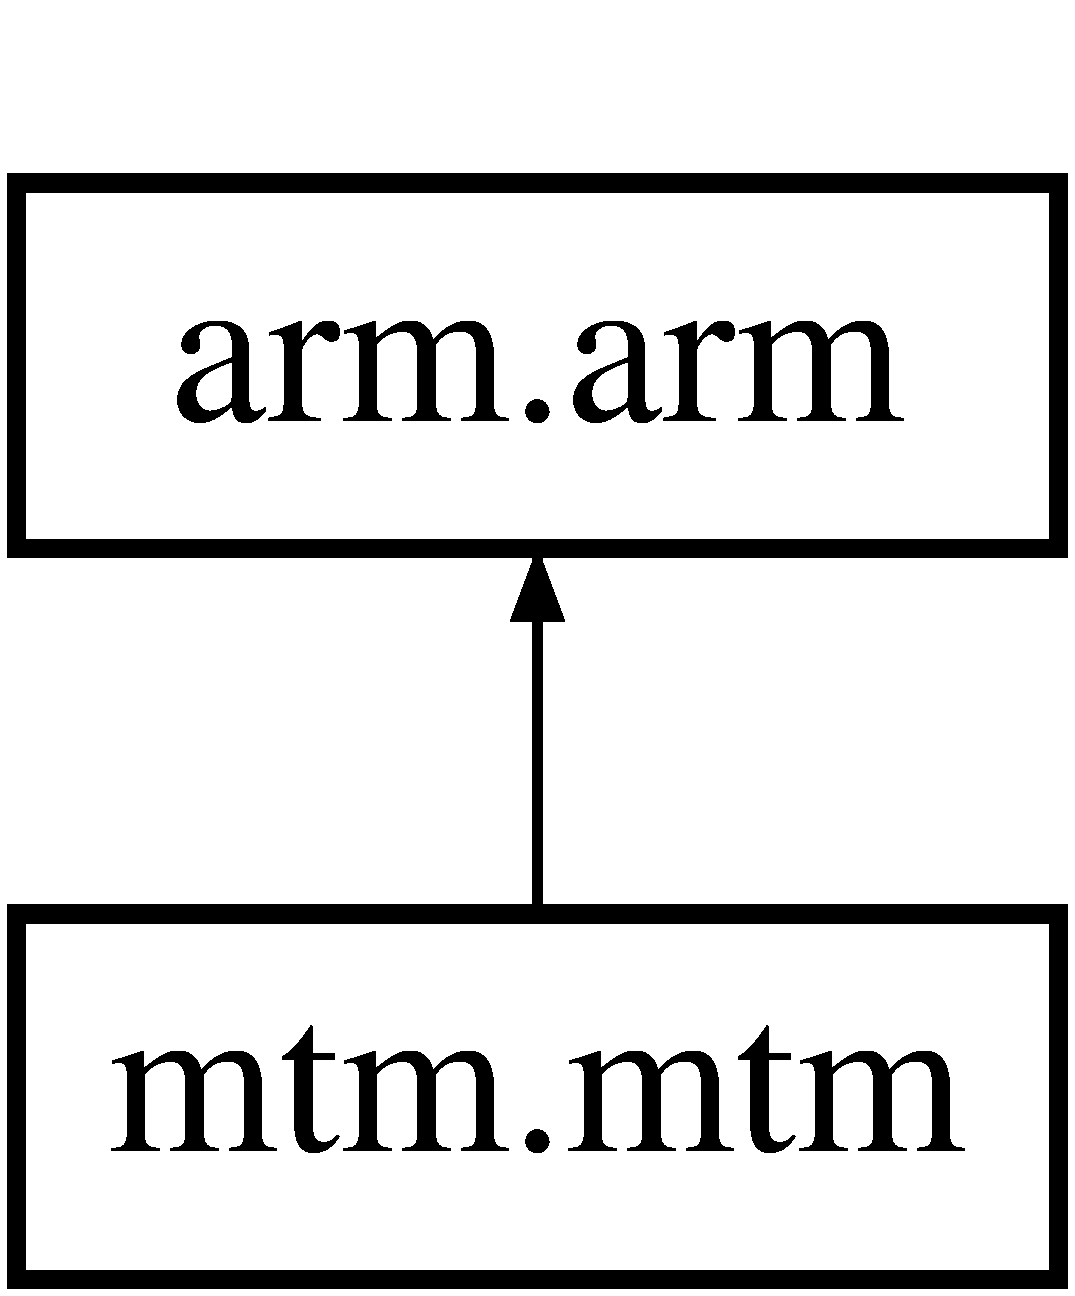
\includegraphics[height=2.000000cm]{classarm_1_1arm}
\end{center}
\end{figure}
\subsection*{Public Member Functions}
\begin{DoxyCompactItemize}
\item 
\hypertarget{classarm_1_1arm_ae08fed39eb81fce7b503f70c5f7b32db}{def {\bfseries \-\_\-\-\_\-init\-\_\-\-\_\-}}\label{classarm_1_1arm_ae08fed39eb81fce7b503f70c5f7b32db}

\item 
\hypertarget{classarm_1_1arm_a8fb4145757c91c0140de04f95cbe69a9}{def {\bfseries unregister}}\label{classarm_1_1arm_a8fb4145757c91c0140de04f95cbe69a9}

\item 
\hypertarget{classarm_1_1arm_a9af25984214c9726ebc9aabf05141b00}{def {\bfseries get\-\_\-robot\-\_\-state}}\label{classarm_1_1arm_a9af25984214c9726ebc9aabf05141b00}

\item 
\hypertarget{classarm_1_1arm_a76a381c30cd928e72fc4ccf3d676792e}{def {\bfseries dvrk\-\_\-set\-\_\-state}}\label{classarm_1_1arm_a76a381c30cd928e72fc4ccf3d676792e}

\item 
def \hyperlink{classarm_1_1arm_a33acf6c2ffac64781467aa9c0a18f55a}{home}
\item 
def \hyperlink{classarm_1_1arm_a7c6d6815fd5a2775ec992aadc083ecd7}{shutdown}
\item 
\hypertarget{classarm_1_1arm_a9af25984214c9726ebc9aabf05141b00}{def {\bfseries get\-\_\-robot\-\_\-state}}\label{classarm_1_1arm_a9af25984214c9726ebc9aabf05141b00}

\item 
def \hyperlink{classarm_1_1arm_ac893260c5e3edc669db9c4b8658f41b5}{get\-\_\-current\-\_\-cartesian\-\_\-position}
\item 
def \hyperlink{classarm_1_1arm_a7bea36edebe3da880a74ec93143a6c75}{get\-\_\-current\-\_\-joint\-\_\-position}
\item 
def \hyperlink{classarm_1_1arm_a0bd1909fb2e302139bf0e4fac8ae456a}{get\-\_\-current\-\_\-joint\-\_\-velocity}
\item 
def \hyperlink{classarm_1_1arm_ae735b4510a3ef3a27b354a6d569907a6}{get\-\_\-current\-\_\-joint\-\_\-effort}
\item 
def \hyperlink{classarm_1_1arm_ab1b18a438ae056c2ba3e845ec2d5216d}{get\-\_\-desired\-\_\-cartesian\-\_\-position}
\item 
def \hyperlink{classarm_1_1arm_a690f5778bad590b39daa32676bbf3182}{get\-\_\-desired\-\_\-joint\-\_\-position}
\item 
def \hyperlink{classarm_1_1arm_a6f56c0ea86dbc842477a68d1da2ac8f6}{get\-\_\-desired\-\_\-joint\-\_\-effort}
\item 
def \hyperlink{classarm_1_1arm_ae80a7d886ac4ea721b4f5df9154f71e4}{get\-\_\-joint\-\_\-number}
\item 
def \hyperlink{classarm_1_1arm_a535bf7aba9ae2891e0a4001cf03661eb}{delta\-\_\-move\-\_\-cartesian}
\item 
def \hyperlink{classarm_1_1arm_aa0cd1135ad795d39ab9475d4f93615bd}{delta\-\_\-move\-\_\-cartesian\-\_\-translation}
\item 
def \hyperlink{classarm_1_1arm_a04ee6edf5b8efe4db259ec7c4f57ee27}{delta\-\_\-move\-\_\-cartesian\-\_\-rotation}
\item 
def \hyperlink{classarm_1_1arm_a0a8751d7ea8ed4ddaf189aed05d72056}{delta\-\_\-move\-\_\-cartesian\-\_\-frame}
\item 
def \hyperlink{classarm_1_1arm_aadb93a6723fb938b75179c1099aa0eca}{move\-\_\-cartesian\-\_\-translation}
\item 
def \hyperlink{classarm_1_1arm_abe86423b4ee21e10d4f45e9dcd92e847}{move\-\_\-cartesian}
\item 
def \hyperlink{classarm_1_1arm_a121642945982da05247c1503fd0a12b9}{move\-\_\-cartesian\-\_\-rotation}
\item 
def \hyperlink{classarm_1_1arm_abfd2494a98ab9cfaccbf4f45f752853e}{move\-\_\-cartesian\-\_\-frame}
\item 
def \hyperlink{classarm_1_1arm_ac483a643a773ab9e14f95c8ec6bdd80a}{delta\-\_\-move\-\_\-joint\-\_\-list}
\item 
def \hyperlink{classarm_1_1arm_a4df0b8f7f9c390f088198f742a340b4a}{move\-\_\-joint\-\_\-list}
\item 
\hypertarget{classarm_1_1arm_aec0abfdbbb95bd56b226ebbf01067b16}{def {\bfseries set\-\_\-wrench\-\_\-spatial\-\_\-force}}\label{classarm_1_1arm_aec0abfdbbb95bd56b226ebbf01067b16}

\item 
\hypertarget{classarm_1_1arm_a7618e46b1cc3e78223a380916b4a1b5f}{def {\bfseries set\-\_\-wrench\-\_\-body\-\_\-orientation\-\_\-absolute}}\label{classarm_1_1arm_a7618e46b1cc3e78223a380916b4a1b5f}

\item 
\hypertarget{classarm_1_1arm_a4f82912fa4e339d843797fa2cd081e21}{def {\bfseries set\-\_\-wrench\-\_\-body\-\_\-force}}\label{classarm_1_1arm_a4f82912fa4e339d843797fa2cd081e21}

\item 
\hypertarget{classarm_1_1arm_a43aa38c319efe3c76d1de2c7f37c49de}{def {\bfseries set\-\_\-gravity\-\_\-compensation}}\label{classarm_1_1arm_a43aa38c319efe3c76d1de2c7f37c49de}

\end{DoxyCompactItemize}
\subsection*{Public Attributes}
\begin{DoxyCompactItemize}
\item 
\hypertarget{classarm_1_1arm_a3af4a73708304dfb539ce3a0b34477a3}{{\bfseries set\-\_\-robot\-\_\-state\-\_\-publisher}}\label{classarm_1_1arm_a3af4a73708304dfb539ce3a0b34477a3}

\item 
\hypertarget{classarm_1_1arm_a3b69cb95dabe0d299c5df1587f777324}{{\bfseries set\-\_\-position\-\_\-joint\-\_\-publisher}}\label{classarm_1_1arm_a3b69cb95dabe0d299c5df1587f777324}

\item 
\hypertarget{classarm_1_1arm_af091f81c9b8f0e3d840007e9a58cc783}{{\bfseries set\-\_\-position\-\_\-goal\-\_\-joint\-\_\-publisher}}\label{classarm_1_1arm_af091f81c9b8f0e3d840007e9a58cc783}

\item 
\hypertarget{classarm_1_1arm_a49910ed075b7bc8b59299ef12d1b574a}{{\bfseries set\-\_\-position\-\_\-cartesian\-\_\-publisher}}\label{classarm_1_1arm_a49910ed075b7bc8b59299ef12d1b574a}

\item 
\hypertarget{classarm_1_1arm_a97437865e96c6505b4cb96510b1fabc2}{{\bfseries set\-\_\-position\-\_\-goal\-\_\-cartesian\-\_\-publisher}}\label{classarm_1_1arm_a97437865e96c6505b4cb96510b1fabc2}

\item 
\hypertarget{classarm_1_1arm_a9ec118079a66acd8ce413bd84d13ac4d}{{\bfseries set\-\_\-wrench\-\_\-body\-\_\-publisher}}\label{classarm_1_1arm_a9ec118079a66acd8ce413bd84d13ac4d}

\item 
\hypertarget{classarm_1_1arm_a307144d2dbb872474841694dc9769645}{{\bfseries set\-\_\-wrench\-\_\-body\-\_\-orientation\-\_\-absolute\-\_\-publisher}}\label{classarm_1_1arm_a307144d2dbb872474841694dc9769645}

\item 
\hypertarget{classarm_1_1arm_ad56c26e45bdc6da624e3d33faf919659}{{\bfseries set\-\_\-wrench\-\_\-spatial\-\_\-publisher}}\label{classarm_1_1arm_ad56c26e45bdc6da624e3d33faf919659}

\item 
\hypertarget{classarm_1_1arm_a1822b878d25777ec4d7c88d0f9521ae3}{{\bfseries set\-\_\-gravity\-\_\-compensation\-\_\-publisher}}\label{classarm_1_1arm_a1822b878d25777ec4d7c88d0f9521ae3}

\item 
\hypertarget{classarm_1_1arm_a2619fc7825f909121b8942360d70cb64}{{\bfseries sub\-\_\-robot\-\_\-state}}\label{classarm_1_1arm_a2619fc7825f909121b8942360d70cb64}

\item 
\hypertarget{classarm_1_1arm_a94664c7134e91e050fd828a113a9b8e9}{{\bfseries sub\-\_\-goal\-\_\-reached}}\label{classarm_1_1arm_a94664c7134e91e050fd828a113a9b8e9}

\item 
\hypertarget{classarm_1_1arm_ab188b6652f6e2731a25816f8ef726084}{{\bfseries sub\-\_\-state\-\_\-joint\-\_\-desired}}\label{classarm_1_1arm_ab188b6652f6e2731a25816f8ef726084}

\item 
\hypertarget{classarm_1_1arm_a87d73921e87152a147177a3f30f35730}{{\bfseries sub\-\_\-position\-\_\-cartesian\-\_\-desired}}\label{classarm_1_1arm_a87d73921e87152a147177a3f30f35730}

\item 
\hypertarget{classarm_1_1arm_a03ffc36c0c9009cd896a6f215794021c}{{\bfseries sub\-\_\-state\-\_\-joint\-\_\-current}}\label{classarm_1_1arm_a03ffc36c0c9009cd896a6f215794021c}

\item 
\hypertarget{classarm_1_1arm_a408c9c78635fe7a98368e54ffd5fec4a}{{\bfseries sub\-\_\-position\-\_\-cartesian\-\_\-current}}\label{classarm_1_1arm_a408c9c78635fe7a98368e54ffd5fec4a}

\end{DoxyCompactItemize}


\subsection{Detailed Description}
\begin{DoxyVerb}Simple arm API wrapping around ROS messages
\end{DoxyVerb}
 

\subsection{Member Function Documentation}
\hypertarget{classarm_1_1arm_a535bf7aba9ae2891e0a4001cf03661eb}{\index{arm\-::arm@{arm\-::arm}!delta\-\_\-move\-\_\-cartesian@{delta\-\_\-move\-\_\-cartesian}}
\index{delta\-\_\-move\-\_\-cartesian@{delta\-\_\-move\-\_\-cartesian}!arm::arm@{arm\-::arm}}
\subsubsection[{delta\-\_\-move\-\_\-cartesian}]{\setlength{\rightskip}{0pt plus 5cm}def arm.\-arm.\-delta\-\_\-move\-\_\-cartesian (
\begin{DoxyParamCaption}
\item[{}]{self, }
\item[{}]{delta\-\_\-input, }
\item[{}]{interpolate = {\ttfamily True}}
\end{DoxyParamCaption}
)}}\label{classarm_1_1arm_a535bf7aba9ae2891e0a4001cf03661eb}
\begin{DoxyVerb}Incremental motion in cartesian space.

:param delta_input: the incremental motion you want to make
:param interpolate: see  :ref:`interpolate <interpolate>`
\end{DoxyVerb}
 \hypertarget{classarm_1_1arm_a0a8751d7ea8ed4ddaf189aed05d72056}{\index{arm\-::arm@{arm\-::arm}!delta\-\_\-move\-\_\-cartesian\-\_\-frame@{delta\-\_\-move\-\_\-cartesian\-\_\-frame}}
\index{delta\-\_\-move\-\_\-cartesian\-\_\-frame@{delta\-\_\-move\-\_\-cartesian\-\_\-frame}!arm::arm@{arm\-::arm}}
\subsubsection[{delta\-\_\-move\-\_\-cartesian\-\_\-frame}]{\setlength{\rightskip}{0pt plus 5cm}def arm.\-arm.\-delta\-\_\-move\-\_\-cartesian\-\_\-frame (
\begin{DoxyParamCaption}
\item[{}]{self, }
\item[{}]{delta\-\_\-frame, }
\item[{}]{interpolate = {\ttfamily True}}
\end{DoxyParamCaption}
)}}\label{classarm_1_1arm_a0a8751d7ea8ed4ddaf189aed05d72056}
\begin{DoxyVerb}Incremental move by Frame in cartesian plane.

:param delta_frame: the incremental `PyKDL.Frame <http://docs.ros.org/diamondback/api/kdl/html/python/geometric_primitives.html>`_ based upon the current position
:param interpolate: see  :ref:`interpolate <interpolate>`\end{DoxyVerb}
 \hypertarget{classarm_1_1arm_a04ee6edf5b8efe4db259ec7c4f57ee27}{\index{arm\-::arm@{arm\-::arm}!delta\-\_\-move\-\_\-cartesian\-\_\-rotation@{delta\-\_\-move\-\_\-cartesian\-\_\-rotation}}
\index{delta\-\_\-move\-\_\-cartesian\-\_\-rotation@{delta\-\_\-move\-\_\-cartesian\-\_\-rotation}!arm::arm@{arm\-::arm}}
\subsubsection[{delta\-\_\-move\-\_\-cartesian\-\_\-rotation}]{\setlength{\rightskip}{0pt plus 5cm}def arm.\-arm.\-delta\-\_\-move\-\_\-cartesian\-\_\-rotation (
\begin{DoxyParamCaption}
\item[{}]{self, }
\item[{}]{delta\-\_\-rotation, }
\item[{}]{interpolate = {\ttfamily True}}
\end{DoxyParamCaption}
)}}\label{classarm_1_1arm_a04ee6edf5b8efe4db259ec7c4f57ee27}
\begin{DoxyVerb}Incremental rotation in cartesian plane.

:param delta_rotation: the incremental `PyKDL.Rotation <http://docs.ros.org/diamondback/api/kdl/html/python/geometric_primitives.html>`_ based upon the current position
:param interpolate: see  :ref:`interpolate <interpolate>`\end{DoxyVerb}
 \hypertarget{classarm_1_1arm_aa0cd1135ad795d39ab9475d4f93615bd}{\index{arm\-::arm@{arm\-::arm}!delta\-\_\-move\-\_\-cartesian\-\_\-translation@{delta\-\_\-move\-\_\-cartesian\-\_\-translation}}
\index{delta\-\_\-move\-\_\-cartesian\-\_\-translation@{delta\-\_\-move\-\_\-cartesian\-\_\-translation}!arm::arm@{arm\-::arm}}
\subsubsection[{delta\-\_\-move\-\_\-cartesian\-\_\-translation}]{\setlength{\rightskip}{0pt plus 5cm}def arm.\-arm.\-delta\-\_\-move\-\_\-cartesian\-\_\-translation (
\begin{DoxyParamCaption}
\item[{}]{self, }
\item[{}]{delta\-\_\-translation, }
\item[{}]{interpolate = {\ttfamily True}}
\end{DoxyParamCaption}
)}}\label{classarm_1_1arm_aa0cd1135ad795d39ab9475d4f93615bd}
\begin{DoxyVerb}Incremental translation in cartesian space.

:param delta_translation: the incremental translation you want to make based on the current position, this is in terms of a  `PyKDL.Vector <http://docs.ros.org/diamondback/api/kdl/html/python/geometric_primitives.html>`_ or a list of floats of size 3
:param interpolate: see  :ref:`interpolate <interpolate>`\end{DoxyVerb}
 \hypertarget{classarm_1_1arm_ac483a643a773ab9e14f95c8ec6bdd80a}{\index{arm\-::arm@{arm\-::arm}!delta\-\_\-move\-\_\-joint\-\_\-list@{delta\-\_\-move\-\_\-joint\-\_\-list}}
\index{delta\-\_\-move\-\_\-joint\-\_\-list@{delta\-\_\-move\-\_\-joint\-\_\-list}!arm::arm@{arm\-::arm}}
\subsubsection[{delta\-\_\-move\-\_\-joint\-\_\-list}]{\setlength{\rightskip}{0pt plus 5cm}def arm.\-arm.\-delta\-\_\-move\-\_\-joint\-\_\-list (
\begin{DoxyParamCaption}
\item[{}]{self, }
\item[{}]{value, }
\item[{}]{index = {\ttfamily \mbox{[}\mbox{]}}, }
\item[{}]{interpolate = {\ttfamily True}}
\end{DoxyParamCaption}
)}}\label{classarm_1_1arm_ac483a643a773ab9e14f95c8ec6bdd80a}
\begin{DoxyVerb}Incremental index move in joint space.

:param value: the incremental amount in which you want to move index by, this is a list
:param index: the joint you want to move, this is a list
:param interpolate: see  :ref:`interpolate <interpolate>`\end{DoxyVerb}
 \hypertarget{classarm_1_1arm_ac893260c5e3edc669db9c4b8658f41b5}{\index{arm\-::arm@{arm\-::arm}!get\-\_\-current\-\_\-cartesian\-\_\-position@{get\-\_\-current\-\_\-cartesian\-\_\-position}}
\index{get\-\_\-current\-\_\-cartesian\-\_\-position@{get\-\_\-current\-\_\-cartesian\-\_\-position}!arm::arm@{arm\-::arm}}
\subsubsection[{get\-\_\-current\-\_\-cartesian\-\_\-position}]{\setlength{\rightskip}{0pt plus 5cm}def arm.\-arm.\-get\-\_\-current\-\_\-cartesian\-\_\-position (
\begin{DoxyParamCaption}
\item[{}]{self}
\end{DoxyParamCaption}
)}}\label{classarm_1_1arm_ac893260c5e3edc669db9c4b8658f41b5}
\begin{DoxyVerb}Gets the :ref:`current cartesian position <currentvdesired>` of the arm in terms of cartesian space.

:returns: the current position of the arm in cartesian space
:rtype: `PyKDL.Frame <http://docs.ros.org/diamondback/api/kdl/html/python/geometric_primitives.html>`_\end{DoxyVerb}
 \hypertarget{classarm_1_1arm_ae735b4510a3ef3a27b354a6d569907a6}{\index{arm\-::arm@{arm\-::arm}!get\-\_\-current\-\_\-joint\-\_\-effort@{get\-\_\-current\-\_\-joint\-\_\-effort}}
\index{get\-\_\-current\-\_\-joint\-\_\-effort@{get\-\_\-current\-\_\-joint\-\_\-effort}!arm::arm@{arm\-::arm}}
\subsubsection[{get\-\_\-current\-\_\-joint\-\_\-effort}]{\setlength{\rightskip}{0pt plus 5cm}def arm.\-arm.\-get\-\_\-current\-\_\-joint\-\_\-effort (
\begin{DoxyParamCaption}
\item[{}]{self}
\end{DoxyParamCaption}
)}}\label{classarm_1_1arm_ae735b4510a3ef3a27b354a6d569907a6}
\begin{DoxyVerb}Gets the :ref:`current joint effort <currentvdesired>` of the arm in terms of joint space.

:returns: the current position of the arm in joint space
:rtype: `JointState <http://docs.ros.org/api/sensor_msgs/html/msg/JointState.html>`_\end{DoxyVerb}
 \hypertarget{classarm_1_1arm_a7bea36edebe3da880a74ec93143a6c75}{\index{arm\-::arm@{arm\-::arm}!get\-\_\-current\-\_\-joint\-\_\-position@{get\-\_\-current\-\_\-joint\-\_\-position}}
\index{get\-\_\-current\-\_\-joint\-\_\-position@{get\-\_\-current\-\_\-joint\-\_\-position}!arm::arm@{arm\-::arm}}
\subsubsection[{get\-\_\-current\-\_\-joint\-\_\-position}]{\setlength{\rightskip}{0pt plus 5cm}def arm.\-arm.\-get\-\_\-current\-\_\-joint\-\_\-position (
\begin{DoxyParamCaption}
\item[{}]{self}
\end{DoxyParamCaption}
)}}\label{classarm_1_1arm_a7bea36edebe3da880a74ec93143a6c75}
\begin{DoxyVerb}Gets the :ref:`current joint position <currentvdesired>` of the arm in terms of joint space.

:returns: the current position of the arm in joint space
:rtype: `JointState <http://docs.ros.org/api/sensor_msgs/html/msg/JointState.html>`_\end{DoxyVerb}
 \hypertarget{classarm_1_1arm_a0bd1909fb2e302139bf0e4fac8ae456a}{\index{arm\-::arm@{arm\-::arm}!get\-\_\-current\-\_\-joint\-\_\-velocity@{get\-\_\-current\-\_\-joint\-\_\-velocity}}
\index{get\-\_\-current\-\_\-joint\-\_\-velocity@{get\-\_\-current\-\_\-joint\-\_\-velocity}!arm::arm@{arm\-::arm}}
\subsubsection[{get\-\_\-current\-\_\-joint\-\_\-velocity}]{\setlength{\rightskip}{0pt plus 5cm}def arm.\-arm.\-get\-\_\-current\-\_\-joint\-\_\-velocity (
\begin{DoxyParamCaption}
\item[{}]{self}
\end{DoxyParamCaption}
)}}\label{classarm_1_1arm_a0bd1909fb2e302139bf0e4fac8ae456a}
\begin{DoxyVerb}Gets the :ref:`current joint velocity <currentvdesired>` of the arm in terms of joint space.

:returns: the current position of the arm in joint space
:rtype: `JointState <http://docs.ros.org/api/sensor_msgs/html/msg/JointState.html>`_\end{DoxyVerb}
 \hypertarget{classarm_1_1arm_ab1b18a438ae056c2ba3e845ec2d5216d}{\index{arm\-::arm@{arm\-::arm}!get\-\_\-desired\-\_\-cartesian\-\_\-position@{get\-\_\-desired\-\_\-cartesian\-\_\-position}}
\index{get\-\_\-desired\-\_\-cartesian\-\_\-position@{get\-\_\-desired\-\_\-cartesian\-\_\-position}!arm::arm@{arm\-::arm}}
\subsubsection[{get\-\_\-desired\-\_\-cartesian\-\_\-position}]{\setlength{\rightskip}{0pt plus 5cm}def arm.\-arm.\-get\-\_\-desired\-\_\-cartesian\-\_\-position (
\begin{DoxyParamCaption}
\item[{}]{self}
\end{DoxyParamCaption}
)}}\label{classarm_1_1arm_ab1b18a438ae056c2ba3e845ec2d5216d}
\begin{DoxyVerb}Get the :ref:`desired cartesian position <currentvdesired>` of the arm in terms of caretsian space.

:returns: the desired position of the arm in cartesian space
:rtype: `PyKDL.Frame <http://docs.ros.org/diamondback/api/kdl/html/python/geometric_primitives.html>`_\end{DoxyVerb}
 \hypertarget{classarm_1_1arm_a6f56c0ea86dbc842477a68d1da2ac8f6}{\index{arm\-::arm@{arm\-::arm}!get\-\_\-desired\-\_\-joint\-\_\-effort@{get\-\_\-desired\-\_\-joint\-\_\-effort}}
\index{get\-\_\-desired\-\_\-joint\-\_\-effort@{get\-\_\-desired\-\_\-joint\-\_\-effort}!arm::arm@{arm\-::arm}}
\subsubsection[{get\-\_\-desired\-\_\-joint\-\_\-effort}]{\setlength{\rightskip}{0pt plus 5cm}def arm.\-arm.\-get\-\_\-desired\-\_\-joint\-\_\-effort (
\begin{DoxyParamCaption}
\item[{}]{self}
\end{DoxyParamCaption}
)}}\label{classarm_1_1arm_a6f56c0ea86dbc842477a68d1da2ac8f6}
\begin{DoxyVerb}Gets the :ref:`desired joint effort <currentvdesired>` of the arm in terms of joint space.

:returns: the desired effort of the arm in joint space
:rtype: `JointState <http://docs.ros.org/api/sensor_msgs/html/msg/JointState.html>`_\end{DoxyVerb}
 \hypertarget{classarm_1_1arm_a690f5778bad590b39daa32676bbf3182}{\index{arm\-::arm@{arm\-::arm}!get\-\_\-desired\-\_\-joint\-\_\-position@{get\-\_\-desired\-\_\-joint\-\_\-position}}
\index{get\-\_\-desired\-\_\-joint\-\_\-position@{get\-\_\-desired\-\_\-joint\-\_\-position}!arm::arm@{arm\-::arm}}
\subsubsection[{get\-\_\-desired\-\_\-joint\-\_\-position}]{\setlength{\rightskip}{0pt plus 5cm}def arm.\-arm.\-get\-\_\-desired\-\_\-joint\-\_\-position (
\begin{DoxyParamCaption}
\item[{}]{self}
\end{DoxyParamCaption}
)}}\label{classarm_1_1arm_a690f5778bad590b39daa32676bbf3182}
\begin{DoxyVerb}Gets the :ref:`desired joint position <currentvdesired>` of the arm in terms of joint space.

:returns: the desired position of the arm in joint space
:rtype: `JointState <http://docs.ros.org/api/sensor_msgs/html/msg/JointState.html>`_\end{DoxyVerb}
 \hypertarget{classarm_1_1arm_ae80a7d886ac4ea721b4f5df9154f71e4}{\index{arm\-::arm@{arm\-::arm}!get\-\_\-joint\-\_\-number@{get\-\_\-joint\-\_\-number}}
\index{get\-\_\-joint\-\_\-number@{get\-\_\-joint\-\_\-number}!arm::arm@{arm\-::arm}}
\subsubsection[{get\-\_\-joint\-\_\-number}]{\setlength{\rightskip}{0pt plus 5cm}def arm.\-arm.\-get\-\_\-joint\-\_\-number (
\begin{DoxyParamCaption}
\item[{}]{self}
\end{DoxyParamCaption}
)}}\label{classarm_1_1arm_ae80a7d886ac4ea721b4f5df9154f71e4}
\begin{DoxyVerb}Gets the number of joints on the arm specified.

:returns: the number of joints on the specified arm
:rtype: int\end{DoxyVerb}
 \hypertarget{classarm_1_1arm_a33acf6c2ffac64781467aa9c0a18f55a}{\index{arm\-::arm@{arm\-::arm}!home@{home}}
\index{home@{home}!arm::arm@{arm\-::arm}}
\subsubsection[{home}]{\setlength{\rightskip}{0pt plus 5cm}def arm.\-arm.\-home (
\begin{DoxyParamCaption}
\item[{}]{self}
\end{DoxyParamCaption}
)}}\label{classarm_1_1arm_a33acf6c2ffac64781467aa9c0a18f55a}
\begin{DoxyVerb}This method will provide power to the arm as will as home
the arm. This method requries the arm name.\end{DoxyVerb}
 \hypertarget{classarm_1_1arm_abe86423b4ee21e10d4f45e9dcd92e847}{\index{arm\-::arm@{arm\-::arm}!move\-\_\-cartesian@{move\-\_\-cartesian}}
\index{move\-\_\-cartesian@{move\-\_\-cartesian}!arm::arm@{arm\-::arm}}
\subsubsection[{move\-\_\-cartesian}]{\setlength{\rightskip}{0pt plus 5cm}def arm.\-arm.\-move\-\_\-cartesian (
\begin{DoxyParamCaption}
\item[{}]{self, }
\item[{}]{abs\-\_\-input, }
\item[{}]{interpolate = {\ttfamily True}}
\end{DoxyParamCaption}
)}}\label{classarm_1_1arm_abe86423b4ee21e10d4f45e9dcd92e847}
\begin{DoxyVerb}Absolute translation in cartesian space.

:param abs_input: the absolute translation you want to make
:param interpolate: see  :ref:`interpolate <interpolate>`\end{DoxyVerb}
 \hypertarget{classarm_1_1arm_abfd2494a98ab9cfaccbf4f45f752853e}{\index{arm\-::arm@{arm\-::arm}!move\-\_\-cartesian\-\_\-frame@{move\-\_\-cartesian\-\_\-frame}}
\index{move\-\_\-cartesian\-\_\-frame@{move\-\_\-cartesian\-\_\-frame}!arm::arm@{arm\-::arm}}
\subsubsection[{move\-\_\-cartesian\-\_\-frame}]{\setlength{\rightskip}{0pt plus 5cm}def arm.\-arm.\-move\-\_\-cartesian\-\_\-frame (
\begin{DoxyParamCaption}
\item[{}]{self, }
\item[{}]{abs\-\_\-frame, }
\item[{}]{interpolate = {\ttfamily True}}
\end{DoxyParamCaption}
)}}\label{classarm_1_1arm_abfd2494a98ab9cfaccbf4f45f752853e}
\begin{DoxyVerb}Absolute move by Frame in cartesian plane.

:param abs_frame: the absolute `PyKDL.Frame <http://docs.ros.org/diamondback/api/kdl/html/python/geometric_primitives.html>`_
:param interpolate: see  :ref:`interpolate <interpolate>`\end{DoxyVerb}
 \hypertarget{classarm_1_1arm_a121642945982da05247c1503fd0a12b9}{\index{arm\-::arm@{arm\-::arm}!move\-\_\-cartesian\-\_\-rotation@{move\-\_\-cartesian\-\_\-rotation}}
\index{move\-\_\-cartesian\-\_\-rotation@{move\-\_\-cartesian\-\_\-rotation}!arm::arm@{arm\-::arm}}
\subsubsection[{move\-\_\-cartesian\-\_\-rotation}]{\setlength{\rightskip}{0pt plus 5cm}def arm.\-arm.\-move\-\_\-cartesian\-\_\-rotation (
\begin{DoxyParamCaption}
\item[{}]{self, }
\item[{}]{abs\-\_\-rotation, }
\item[{}]{interpolate = {\ttfamily True}}
\end{DoxyParamCaption}
)}}\label{classarm_1_1arm_a121642945982da05247c1503fd0a12b9}
\begin{DoxyVerb}Absolute rotation in cartesian plane.

:param abs_rotation: the absolute `PyKDL.Rotation <http://docs.ros.org/diamondback/api/kdl/html/python/geometric_primitives.html>`_
:param interpolate: see  :ref:`interpolate <interpolate>`\end{DoxyVerb}
 \hypertarget{classarm_1_1arm_aadb93a6723fb938b75179c1099aa0eca}{\index{arm\-::arm@{arm\-::arm}!move\-\_\-cartesian\-\_\-translation@{move\-\_\-cartesian\-\_\-translation}}
\index{move\-\_\-cartesian\-\_\-translation@{move\-\_\-cartesian\-\_\-translation}!arm::arm@{arm\-::arm}}
\subsubsection[{move\-\_\-cartesian\-\_\-translation}]{\setlength{\rightskip}{0pt plus 5cm}def arm.\-arm.\-move\-\_\-cartesian\-\_\-translation (
\begin{DoxyParamCaption}
\item[{}]{self, }
\item[{}]{abs\-\_\-translation, }
\item[{}]{interpolate = {\ttfamily True}}
\end{DoxyParamCaption}
)}}\label{classarm_1_1arm_aadb93a6723fb938b75179c1099aa0eca}
\begin{DoxyVerb}Absolute translation in cartesian space.

:param abs_translation: the absolute translation you want to make, this is in terms of a  `PyKDL.Vector <http://docs.ros.org/diamondback/api/kdl/html/python/geometric_primitives.html>`_ or a list of floats of size 3
:param interpolate: see  :ref:`interpolate <interpolate>`\end{DoxyVerb}
 \hypertarget{classarm_1_1arm_a4df0b8f7f9c390f088198f742a340b4a}{\index{arm\-::arm@{arm\-::arm}!move\-\_\-joint\-\_\-list@{move\-\_\-joint\-\_\-list}}
\index{move\-\_\-joint\-\_\-list@{move\-\_\-joint\-\_\-list}!arm::arm@{arm\-::arm}}
\subsubsection[{move\-\_\-joint\-\_\-list}]{\setlength{\rightskip}{0pt plus 5cm}def arm.\-arm.\-move\-\_\-joint\-\_\-list (
\begin{DoxyParamCaption}
\item[{}]{self, }
\item[{}]{value, }
\item[{}]{index = {\ttfamily \mbox{[}\mbox{]}}, }
\item[{}]{interpolate = {\ttfamily True}}
\end{DoxyParamCaption}
)}}\label{classarm_1_1arm_a4df0b8f7f9c390f088198f742a340b4a}
\begin{DoxyVerb}Absolute index move in joint space.

:param value: the incremental amount in which you want to move index by, this is a list
:param index: the incremental joint you want to move, this is a list
:param interpolate: see  :ref:`interpolate <interpolate>`\end{DoxyVerb}
 \hypertarget{classarm_1_1arm_a7c6d6815fd5a2775ec992aadc083ecd7}{\index{arm\-::arm@{arm\-::arm}!shutdown@{shutdown}}
\index{shutdown@{shutdown}!arm::arm@{arm\-::arm}}
\subsubsection[{shutdown}]{\setlength{\rightskip}{0pt plus 5cm}def arm.\-arm.\-shutdown (
\begin{DoxyParamCaption}
\item[{}]{self}
\end{DoxyParamCaption}
)}}\label{classarm_1_1arm_a7c6d6815fd5a2775ec992aadc083ecd7}
\begin{DoxyVerb}Stops providing power to the arm.\end{DoxyVerb}
 

The documentation for this class was generated from the following file\-:\begin{DoxyCompactItemize}
\item 
arm.\-py\end{DoxyCompactItemize}

\hypertarget{classautocamera__algorithm_1_1Autocamera}{\section{autocamera\-\_\-algorithm.\-Autocamera Class Reference}
\label{classautocamera__algorithm_1_1Autocamera}\index{autocamera\-\_\-algorithm.\-Autocamera@{autocamera\-\_\-algorithm.\-Autocamera}}
}
\subsection*{Public Member Functions}
\begin{DoxyCompactItemize}
\item 
\hypertarget{classautocamera__algorithm_1_1Autocamera_a88d53452675d2b51c312bd76c5a46dfb}{def {\bfseries \-\_\-\-\_\-init\-\_\-\-\_\-}}\label{classautocamera__algorithm_1_1Autocamera_a88d53452675d2b51c312bd76c5a46dfb}

\item 
\hypertarget{classautocamera__algorithm_1_1Autocamera_a107fbd8731769063038b861fe06cd904}{def {\bfseries logerror}}\label{classautocamera__algorithm_1_1Autocamera_a107fbd8731769063038b861fe06cd904}

\item 
\hypertarget{classautocamera__algorithm_1_1Autocamera_a741362e4cf80c27b87f2f74e1f9da4ef}{def {\bfseries dotproduct}}\label{classautocamera__algorithm_1_1Autocamera_a741362e4cf80c27b87f2f74e1f9da4ef}

\item 
\hypertarget{classautocamera__algorithm_1_1Autocamera_af90f7c97b8863d2bbdac99f88b7cb3b8}{def {\bfseries length}}\label{classautocamera__algorithm_1_1Autocamera_af90f7c97b8863d2bbdac99f88b7cb3b8}

\item 
\hypertarget{classautocamera__algorithm_1_1Autocamera_abeb1602619307de1f9b7b37503fd90d3}{def {\bfseries angle}}\label{classautocamera__algorithm_1_1Autocamera_abeb1602619307de1f9b7b37503fd90d3}

\item 
\hypertarget{classautocamera__algorithm_1_1Autocamera_a989fda868dbc2caa0fc3b48c787c2484}{def {\bfseries column}}\label{classautocamera__algorithm_1_1Autocamera_a989fda868dbc2caa0fc3b48c787c2484}

\item 
\hypertarget{classautocamera__algorithm_1_1Autocamera_a7170368dd1031e799f4eacb3fb859d30}{def {\bfseries find\-\_\-rotation\-\_\-matrix\-\_\-between\-\_\-two\-\_\-vectors}}\label{classautocamera__algorithm_1_1Autocamera_a7170368dd1031e799f4eacb3fb859d30}

\item 
\hypertarget{classautocamera__algorithm_1_1Autocamera_aa53bae6eea8aae0a233a7886549039f2}{def {\bfseries extract\-\_\-positions}}\label{classautocamera__algorithm_1_1Autocamera_aa53bae6eea8aae0a233a7886549039f2}

\item 
\hypertarget{classautocamera__algorithm_1_1Autocamera_a6344825a1f6ebc37210ae6900d142ccd}{def {\bfseries add\-\_\-marker}}\label{classautocamera__algorithm_1_1Autocamera_a6344825a1f6ebc37210ae6900d142ccd}

\item 
\hypertarget{classautocamera__algorithm_1_1Autocamera_ac8bcb5e780d60fc89a01954355336b43}{def {\bfseries point\-\_\-towards\-\_\-midpoint}}\label{classautocamera__algorithm_1_1Autocamera_ac8bcb5e780d60fc89a01954355336b43}

\item 
\hypertarget{classautocamera__algorithm_1_1Autocamera_a5b3cd46a598ddb9a94a92fc1f2a81def}{def {\bfseries find\-\_\-2d\-\_\-tool\-\_\-coordinates\-\_\-in\-\_\-3d}}\label{classautocamera__algorithm_1_1Autocamera_a5b3cd46a598ddb9a94a92fc1f2a81def}

\item 
\hypertarget{classautocamera__algorithm_1_1Autocamera_a99c5c26e53c9caf8b677adc0bdd98d07}{def {\bfseries zoom\-\_\-fitness}}\label{classautocamera__algorithm_1_1Autocamera_a99c5c26e53c9caf8b677adc0bdd98d07}

\item 
\hypertarget{classautocamera__algorithm_1_1Autocamera_a3417f3b93de924c6ce6283e50b8cc1d6}{def {\bfseries zoom\-\_\-fitness2}}\label{classautocamera__algorithm_1_1Autocamera_a3417f3b93de924c6ce6283e50b8cc1d6}

\item 
\hypertarget{classautocamera__algorithm_1_1Autocamera_aaf38b3bac1aeac2afff5c4ed3543f652}{def {\bfseries unrectify\-\_\-point}}\label{classautocamera__algorithm_1_1Autocamera_aaf38b3bac1aeac2afff5c4ed3543f652}

\item 
\hypertarget{classautocamera__algorithm_1_1Autocamera_a22083eb61be00dfbc8edf68b67a13119}{def {\bfseries get\-\_\-2d\-\_\-point\-\_\-from\-\_\-3d\-\_\-point\-\_\-relative\-\_\-to\-\_\-world\-\_\-rf}}\label{classautocamera__algorithm_1_1Autocamera_a22083eb61be00dfbc8edf68b67a13119}

\item 
\hypertarget{classautocamera__algorithm_1_1Autocamera_a37c2f7b8a0409809580f0f82189f7dc1}{def {\bfseries find\-\_\-zoom\-\_\-level}}\label{classautocamera__algorithm_1_1Autocamera_a37c2f7b8a0409809580f0f82189f7dc1}

\item 
\hypertarget{classautocamera__algorithm_1_1Autocamera_aa11750e41b8c8ca3d4123e10f5130e7f}{def {\bfseries track\-\_\-tool\-\_\-times}}\label{classautocamera__algorithm_1_1Autocamera_aa11750e41b8c8ca3d4123e10f5130e7f}

\item 
\hypertarget{classautocamera__algorithm_1_1Autocamera_a72fd3893e82eeedced9aa7abbc82f419}{def {\bfseries compute\-\_\-viewangle}}\label{classautocamera__algorithm_1_1Autocamera_a72fd3893e82eeedced9aa7abbc82f419}

\end{DoxyCompactItemize}
\subsection*{Public Attributes}
\begin{DoxyCompactItemize}
\item 
\hypertarget{classautocamera__algorithm_1_1Autocamera_a8f62f4fcec50e0cefd4e1a835eec3c1d}{{\bfseries ecm\-\_\-robot}}\label{classautocamera__algorithm_1_1Autocamera_a8f62f4fcec50e0cefd4e1a835eec3c1d}

\item 
\hypertarget{classautocamera__algorithm_1_1Autocamera_a920c7f744fc34f472e29e8c8633c40b8}{{\bfseries ecm\-\_\-kin}}\label{classautocamera__algorithm_1_1Autocamera_a920c7f744fc34f472e29e8c8633c40b8}

\item 
\hypertarget{classautocamera__algorithm_1_1Autocamera_a81e7e0a63180e7ab293dd3264f8b9739}{{\bfseries psm1\-\_\-robot}}\label{classautocamera__algorithm_1_1Autocamera_a81e7e0a63180e7ab293dd3264f8b9739}

\item 
\hypertarget{classautocamera__algorithm_1_1Autocamera_af6c262b8ac34acdb7ffe261699f51144}{{\bfseries psm1\-\_\-kin}}\label{classautocamera__algorithm_1_1Autocamera_af6c262b8ac34acdb7ffe261699f51144}

\item 
\hypertarget{classautocamera__algorithm_1_1Autocamera_aff7bc4b23fcb64495144090b1e95ee77}{{\bfseries psm2\-\_\-robot}}\label{classautocamera__algorithm_1_1Autocamera_aff7bc4b23fcb64495144090b1e95ee77}

\item 
\hypertarget{classautocamera__algorithm_1_1Autocamera_a90d52e62a513003bfb99b91692f48f4e}{{\bfseries psm2\-\_\-kin}}\label{classautocamera__algorithm_1_1Autocamera_a90d52e62a513003bfb99b91692f48f4e}

\item 
\hypertarget{classautocamera__algorithm_1_1Autocamera_a93949ede55683a95c7dfebdcf312074d}{{\bfseries zoom\-\_\-percentage}}\label{classautocamera__algorithm_1_1Autocamera_a93949ede55683a95c7dfebdcf312074d}

\item 
\hypertarget{classautocamera__algorithm_1_1Autocamera_a373f87e3f50b817ca0cf6ad69ee7d1a6}{{\bfseries tool\-\_\-timer}}\label{classautocamera__algorithm_1_1Autocamera_a373f87e3f50b817ca0cf6ad69ee7d1a6}

\item 
\hypertarget{classautocamera__algorithm_1_1Autocamera_ac6a3700c6ddbc1054b14e1b5c09e682c}{{\bfseries last\-\_\-midpoint}}\label{classautocamera__algorithm_1_1Autocamera_ac6a3700c6ddbc1054b14e1b5c09e682c}

\item 
\hypertarget{classautocamera__algorithm_1_1Autocamera_a421846b23b25d7dcc2be3c3f0348978a}{{\bfseries midpoint\-\_\-time}}\label{classautocamera__algorithm_1_1Autocamera_a421846b23b25d7dcc2be3c3f0348978a}

\item 
\hypertarget{classautocamera__algorithm_1_1Autocamera_aff068deae80870cc617ef430d4d6590a}{{\bfseries pan\-\_\-tilt\-\_\-deadzone\-\_\-radius}}\label{classautocamera__algorithm_1_1Autocamera_aff068deae80870cc617ef430d4d6590a}

\item 
\hypertarget{classautocamera__algorithm_1_1Autocamera_ac0b17104472e7d33dfe1f66f8bb75357}{{\bfseries zoom\-\_\-deadzone\-\_\-radius}}\label{classautocamera__algorithm_1_1Autocamera_ac0b17104472e7d33dfe1f66f8bb75357}

\item 
\hypertarget{classautocamera__algorithm_1_1Autocamera_a9d166f369baef6ea8265c4d00494a720}{{\bfseries zoom\-\_\-innerzone\-\_\-radius}}\label{classautocamera__algorithm_1_1Autocamera_a9d166f369baef6ea8265c4d00494a720}

\item 
\hypertarget{classautocamera__algorithm_1_1Autocamera_a967fc0fd2c00ed88cd841b267b062833}{{\bfseries zones\-\_\-times}}\label{classautocamera__algorithm_1_1Autocamera_a967fc0fd2c00ed88cd841b267b062833}

\item 
\hypertarget{classautocamera__algorithm_1_1Autocamera_abf93128611ea273d55d49671e59b0614}{{\bfseries zoom\-\_\-level\-\_\-positions}}\label{classautocamera__algorithm_1_1Autocamera_abf93128611ea273d55d49671e59b0614}

\end{DoxyCompactItemize}
\subsection*{Static Public Attributes}
\begin{DoxyCompactItemize}
\item 
\hypertarget{classautocamera__algorithm_1_1Autocamera_a8f958fa5bb7600d9d300e367c907d8eb}{{\bfseries D\-E\-B\-U\-G} = False}\label{classautocamera__algorithm_1_1Autocamera_a8f958fa5bb7600d9d300e367c907d8eb}

\item 
\hypertarget{classautocamera__algorithm_1_1Autocamera_a61c1aff3f5d33b45e334d7f689845bd2}{tuple {\bfseries ig} = image\-\_\-geometry.\-Stereo\-Camera\-Model()}\label{classautocamera__algorithm_1_1Autocamera_a61c1aff3f5d33b45e334d7f689845bd2}

\item 
\hypertarget{classautocamera__algorithm_1_1Autocamera_a4cf82103ade000d5fab46b0967faa93b}{tuple {\bfseries r} = Pose\-Conv.\-to\-\_\-homo\-\_\-mat( \mbox{[} (0.\-0, 0.\-0, 0.\-0), (0.\-0, 0.\-0, 1.\-57079632679) \mbox{]})}\label{classautocamera__algorithm_1_1Autocamera_a4cf82103ade000d5fab46b0967faa93b}

\item 
\hypertarget{classautocamera__algorithm_1_1Autocamera_a95913023e8d85880d30bbca76e0044db}{tuple {\bfseries r\-\_\-inv} = numpy.\-linalg.\-inv(r)}\label{classautocamera__algorithm_1_1Autocamera_a95913023e8d85880d30bbca76e0044db}

\item 
\hypertarget{classautocamera__algorithm_1_1Autocamera_a37bf464128bbbefe8d3f83e65bcb51ad}{tuple {\bfseries mp} = ( int(l1\mbox{[}0\mbox{]}+l2\mbox{[}0\mbox{]})/2, int(l1\mbox{[}1\mbox{]} + l2\mbox{[}1\mbox{]})/2)}\label{classautocamera__algorithm_1_1Autocamera_a37bf464128bbbefe8d3f83e65bcb51ad}

\item 
\hypertarget{classautocamera__algorithm_1_1Autocamera_ab9597b120e0539e35ab615a260fc98df}{tuple {\bfseries P} = numpy.\-array(cam\-\_\-info.\-P)}\label{classautocamera__algorithm_1_1Autocamera_ab9597b120e0539e35ab615a260fc98df}

\item 
\hypertarget{classautocamera__algorithm_1_1Autocamera_a7b3083c9cc2b78e45f270ef16b66c82e}{{\bfseries m} = T\-E\-W\-\_\-inv$\ast$point}\label{classautocamera__algorithm_1_1Autocamera_a7b3083c9cc2b78e45f270ef16b66c82e}

\item 
\hypertarget{classautocamera__algorithm_1_1Autocamera_a9e6aec10c509b20ba0bf5df8e06c4a04}{{\bfseries x} = u/w}\label{classautocamera__algorithm_1_1Autocamera_a9e6aec10c509b20ba0bf5df8e06c4a04}

\item 
\hypertarget{classautocamera__algorithm_1_1Autocamera_a55d96e7c6c384a5a04c149f1ed760c88}{{\bfseries y} = v/w}\label{classautocamera__algorithm_1_1Autocamera_a55d96e7c6c384a5a04c149f1ed760c88}

\item 
\hypertarget{classautocamera__algorithm_1_1Autocamera_a02c21de1e73f6a2459b5785c87d744ef}{int {\bfseries Width} = 640}\label{classautocamera__algorithm_1_1Autocamera_a02c21de1e73f6a2459b5785c87d744ef}

\item 
\hypertarget{classautocamera__algorithm_1_1Autocamera_a9695ec87d723607eb6c15142737f78d0}{int {\bfseries x} = x$\ast$.\-5}\label{classautocamera__algorithm_1_1Autocamera_a9695ec87d723607eb6c15142737f78d0}

\item 
\hypertarget{classautocamera__algorithm_1_1Autocamera_a98c4ce7d9c50bb804a277d545c0c3700}{int {\bfseries y} = y$\ast$.\-5}\label{classautocamera__algorithm_1_1Autocamera_a98c4ce7d9c50bb804a277d545c0c3700}

\item 
tuple {\bfseries zoom\-\_\-percentage}
\item 
\hypertarget{classautocamera__algorithm_1_1Autocamera_aa2132f7e89d44d9a5f02b770f378e4df}{list {\bfseries output\-\_\-msg} = clean\-\_\-joints\mbox{[}'ecm'\mbox{]}}\label{classautocamera__algorithm_1_1Autocamera_aa2132f7e89d44d9a5f02b770f378e4df}

\item 
\hypertarget{classautocamera__algorithm_1_1Autocamera_a276dfc60c57fa3b99bcdf1246c663f24}{tuple {\bfseries gripper} = max( \mbox{[} abs(joint\mbox{[}'psm1'\mbox{]}.position\mbox{[}-\/1\mbox{]}), abs(joint\mbox{[}'psm2'\mbox{]}.position\mbox{[}-\/1\mbox{]})\mbox{]} )}\label{classautocamera__algorithm_1_1Autocamera_a276dfc60c57fa3b99bcdf1246c663f24}

\item 
\hypertarget{classautocamera__algorithm_1_1Autocamera_aa2132f7e89d44d9a5f02b770f378e4df}{tuple {\bfseries output\-\_\-msg} = self.\-point\-\_\-towards\-\_\-midpoint(clean\-\_\-joints, psm1\-\_\-pos, psm2\-\_\-pos, key\-\_\-hole, ecm\-\_\-pose, cam\-\_\-info)}\label{classautocamera__algorithm_1_1Autocamera_aa2132f7e89d44d9a5f02b770f378e4df}

\end{DoxyCompactItemize}


\subsection{Member Data Documentation}
\hypertarget{classautocamera__algorithm_1_1Autocamera_a43fdedb88b14ed5863465f63c1d34a68}{\index{autocamera\-\_\-algorithm\-::\-Autocamera@{autocamera\-\_\-algorithm\-::\-Autocamera}!zoom\-\_\-percentage@{zoom\-\_\-percentage}}
\index{zoom\-\_\-percentage@{zoom\-\_\-percentage}!autocamera_algorithm::Autocamera@{autocamera\-\_\-algorithm\-::\-Autocamera}}
\subsubsection[{zoom\-\_\-percentage}]{\setlength{\rightskip}{0pt plus 5cm}tuple autocamera\-\_\-algorithm.\-Autocamera.\-zoom\-\_\-percentage\hspace{0.3cm}{\ttfamily [static]}}}\label{classautocamera__algorithm_1_1Autocamera_a43fdedb88b14ed5863465f63c1d34a68}
{\bfseries Initial value\-:}
\begin{DoxyCode}
1 = self.zoom\_fitness2(cam\_info[\textcolor{stringliteral}{'left'}], mid\_point=mp, tool\_point=l1, 
2                                             tool\_point2=l2, radius=self.zoom\_innerzone\_radius, 
      deadzone\_radius=self.zoom\_deadzone\_radius)
\end{DoxyCode}


The documentation for this class was generated from the following file\-:\begin{DoxyCompactItemize}
\item 
autocamera\-\_\-algorithm.\-py\end{DoxyCompactItemize}

\hypertarget{classcamera__control__node_1_1Autocamera__node__handler}{\section{camera\-\_\-control\-\_\-node.\-Autocamera\-\_\-node\-\_\-handler Class Reference}
\label{classcamera__control__node_1_1Autocamera__node__handler}\index{camera\-\_\-control\-\_\-node.\-Autocamera\-\_\-node\-\_\-handler@{camera\-\_\-control\-\_\-node.\-Autocamera\-\_\-node\-\_\-handler}}
}
\subsection*{Classes}
\begin{DoxyCompactItemize}
\item 
class \hyperlink{classcamera__control__node_1_1Autocamera__node__handler_1_1MODE}{M\-O\-D\-E}
\end{DoxyCompactItemize}
\subsection*{Public Member Functions}
\begin{DoxyCompactItemize}
\item 
\hypertarget{classcamera__control__node_1_1Autocamera__node__handler_ab58e53ba67d6fb7113e11d7bb88c3b7f}{def {\bfseries \-\_\-\-\_\-init\-\_\-\-\_\-}}\label{classcamera__control__node_1_1Autocamera__node__handler_ab58e53ba67d6fb7113e11d7bb88c3b7f}

\item 
\hypertarget{classcamera__control__node_1_1Autocamera__node__handler_af00c572de6d9670c6d7d75f14fb7b8de}{def {\bfseries \-\_\-\-\_\-init\-\_\-nodes\-\_\-\-\_\-}}\label{classcamera__control__node_1_1Autocamera__node__handler_af00c572de6d9670c6d7d75f14fb7b8de}

\end{DoxyCompactItemize}
\subsection*{Public Attributes}
\begin{DoxyCompactItemize}
\item 
\hypertarget{classcamera__control__node_1_1Autocamera__node__handler_a2a14a1500c1e947027b8dbcf80b3ba5c}{{\bfseries t}}\label{classcamera__control__node_1_1Autocamera__node__handler_a2a14a1500c1e947027b8dbcf80b3ba5c}

\item 
\hypertarget{classcamera__control__node_1_1Autocamera__node__handler_a52d3dec668098ed561babf2085f438f9}{{\bfseries autocamera}}\label{classcamera__control__node_1_1Autocamera__node__handler_a52d3dec668098ed561babf2085f438f9}

\item 
\hypertarget{classcamera__control__node_1_1Autocamera__node__handler_a21e1fee72487e9716df669444cf8de1c}{{\bfseries jnt\-\_\-msg}}\label{classcamera__control__node_1_1Autocamera__node__handler_a21e1fee72487e9716df669444cf8de1c}

\item 
\hypertarget{classcamera__control__node_1_1Autocamera__node__handler_a74d10f9867779759521d29cf998d680c}{{\bfseries joint\-\_\-angles}}\label{classcamera__control__node_1_1Autocamera__node__handler_a74d10f9867779759521d29cf998d680c}

\item 
\hypertarget{classcamera__control__node_1_1Autocamera__node__handler_a7dc91254a8c7869bd27fe0c121db6d44}{{\bfseries cam\-\_\-info}}\label{classcamera__control__node_1_1Autocamera__node__handler_a7dc91254a8c7869bd27fe0c121db6d44}

\item 
\hypertarget{classcamera__control__node_1_1Autocamera__node__handler_a886d5599464713fcc171798a4c4f4c52}{{\bfseries last\-\_\-ecm\-\_\-jnt\-\_\-pos}}\label{classcamera__control__node_1_1Autocamera__node__handler_a886d5599464713fcc171798a4c4f4c52}

\item 
\hypertarget{classcamera__control__node_1_1Autocamera__node__handler_a81e1f12f6178bd42ab80b009ad3b6c02}{{\bfseries first\-\_\-run}}\label{classcamera__control__node_1_1Autocamera__node__handler_a81e1f12f6178bd42ab80b009ad3b6c02}

\item 
\hypertarget{classcamera__control__node_1_1Autocamera__node__handler_a790b04d6dd55bf1e6bc095323d0ba4c5}{{\bfseries headsensor\-\_\-active}}\label{classcamera__control__node_1_1Autocamera__node__handler_a790b04d6dd55bf1e6bc095323d0ba4c5}

\item 
\hypertarget{classcamera__control__node_1_1Autocamera__node__handler_afc7b1559add9f6ea5d8e14f17b57f78c}{{\bfseries repositioning\-\_\-clutch\-\_\-active}}\label{classcamera__control__node_1_1Autocamera__node__handler_afc7b1559add9f6ea5d8e14f17b57f78c}

\item 
\hypertarget{classcamera__control__node_1_1Autocamera__node__handler_ac6095a076ee675ca60d541966d085d93}{{\bfseries camera\-\_\-clutch\-\_\-pressed}}\label{classcamera__control__node_1_1Autocamera__node__handler_ac6095a076ee675ca60d541966d085d93}

\item 
\hypertarget{classcamera__control__node_1_1Autocamera__node__handler_a417c7372211104db3645d7cab0ec970e}{{\bfseries ecm\-\_\-manual\-\_\-control\-\_\-lock\-\_\-mtml\-\_\-msg}}\label{classcamera__control__node_1_1Autocamera__node__handler_a417c7372211104db3645d7cab0ec970e}

\item 
\hypertarget{classcamera__control__node_1_1Autocamera__node__handler_a3f3bdf1337bdb7259262e152f3f4bcaa}{{\bfseries ecm\-\_\-manual\-\_\-control\-\_\-lock\-\_\-ecm\-\_\-msg}}\label{classcamera__control__node_1_1Autocamera__node__handler_a3f3bdf1337bdb7259262e152f3f4bcaa}

\item 
\hypertarget{classcamera__control__node_1_1Autocamera__node__handler_a4747f2b8a1badb166ef89cbcfb8c465b}{{\bfseries mtml\-\_\-start\-\_\-position}}\label{classcamera__control__node_1_1Autocamera__node__handler_a4747f2b8a1badb166ef89cbcfb8c465b}

\item 
\hypertarget{classcamera__control__node_1_1Autocamera__node__handler_a99cb2a1418010711ef2ef6cbb5aafdcb}{{\bfseries mtml\-\_\-end\-\_\-position}}\label{classcamera__control__node_1_1Autocamera__node__handler_a99cb2a1418010711ef2ef6cbb5aafdcb}

\item 
\hypertarget{classcamera__control__node_1_1Autocamera__node__handler_af30eac87ef94d11389e0fcb2b7651e95}{{\bfseries config}}\label{classcamera__control__node_1_1Autocamera__node__handler_af30eac87ef94d11389e0fcb2b7651e95}

\item 
\hypertarget{classcamera__control__node_1_1Autocamera__node__handler_a466239467720aa9ddd7710073216bc07}{{\bfseries config\-\_\-file}}\label{classcamera__control__node_1_1Autocamera__node__handler_a466239467720aa9ddd7710073216bc07}

\item 
\hypertarget{classcamera__control__node_1_1Autocamera__node__handler_a91ce596b91620632c5bf1ad2a339a3ed}{{\bfseries initialize\-\_\-psms\-\_\-initialized}}\label{classcamera__control__node_1_1Autocamera__node__handler_a91ce596b91620632c5bf1ad2a339a3ed}

\item 
\hypertarget{classcamera__control__node_1_1Autocamera__node__handler_a7a6da4afada32ab81222c898e0a1160b}{{\bfseries hw\-\_\-ecm}}\label{classcamera__control__node_1_1Autocamera__node__handler_a7a6da4afada32ab81222c898e0a1160b}

\item 
\hypertarget{classcamera__control__node_1_1Autocamera__node__handler_a14c83e4af8151b9e370c9c8b9b924c11}{{\bfseries pub\-\_\-ecm}}\label{classcamera__control__node_1_1Autocamera__node__handler_a14c83e4af8151b9e370c9c8b9b924c11}

\item 
\hypertarget{classcamera__control__node_1_1Autocamera__node__handler_a5e3e6687620860e11152475ad218a067}{{\bfseries sub\-\_\-ecm\-\_\-sim}}\label{classcamera__control__node_1_1Autocamera__node__handler_a5e3e6687620860e11152475ad218a067}

\item 
\hypertarget{classcamera__control__node_1_1Autocamera__node__handler_a7eed523eb8fdb394ceb7932ed253c70f}{{\bfseries sub\-\_\-caminfo}}\label{classcamera__control__node_1_1Autocamera__node__handler_a7eed523eb8fdb394ceb7932ed253c70f}

\item 
\hypertarget{classcamera__control__node_1_1Autocamera__node__handler_a8fbf799abb8ea251d9cd950a8b836f62}{{\bfseries sub\-\_\-psm1\-\_\-hw}}\label{classcamera__control__node_1_1Autocamera__node__handler_a8fbf799abb8ea251d9cd950a8b836f62}

\item 
\hypertarget{classcamera__control__node_1_1Autocamera__node__handler_a41da05ee892c6aeeab7a6b596efec39f}{{\bfseries sub\-\_\-psm2\-\_\-hw}}\label{classcamera__control__node_1_1Autocamera__node__handler_a41da05ee892c6aeeab7a6b596efec39f}

\item 
\hypertarget{classcamera__control__node_1_1Autocamera__node__handler_ac6277f88ddcc0f99d61749f82ed97de9}{{\bfseries sub\-\_\-headsensor}}\label{classcamera__control__node_1_1Autocamera__node__handler_ac6277f88ddcc0f99d61749f82ed97de9}

\item 
\hypertarget{classcamera__control__node_1_1Autocamera__node__handler_a76dd83fa5802f0bc7cfc7ed3e3635c97}{{\bfseries sub\-\_\-repositioning\-\_\-clutch}}\label{classcamera__control__node_1_1Autocamera__node__handler_a76dd83fa5802f0bc7cfc7ed3e3635c97}

\item 
\hypertarget{classcamera__control__node_1_1Autocamera__node__handler_a8398b5c30ed0deddcf66b6a00ea6fde2}{{\bfseries sub\-\_\-psm1\-\_\-sim}}\label{classcamera__control__node_1_1Autocamera__node__handler_a8398b5c30ed0deddcf66b6a00ea6fde2}

\item 
\hypertarget{classcamera__control__node_1_1Autocamera__node__handler_afe0db682ff11042a4d3659e0d8a698f9}{{\bfseries sub\-\_\-psm2\-\_\-sim}}\label{classcamera__control__node_1_1Autocamera__node__handler_afe0db682ff11042a4d3659e0d8a698f9}

\end{DoxyCompactItemize}


The documentation for this class was generated from the following file\-:\begin{DoxyCompactItemize}
\item 
camera\-\_\-control\-\_\-node.\-py\end{DoxyCompactItemize}

\hypertarget{classrosbag__cmd_1_1bag__reader}{\section{rosbag\-\_\-cmd.\-bag\-\_\-reader Class Reference}
\label{classrosbag__cmd_1_1bag__reader}\index{rosbag\-\_\-cmd.\-bag\-\_\-reader@{rosbag\-\_\-cmd.\-bag\-\_\-reader}}
}
\subsection*{Public Member Functions}
\begin{DoxyCompactItemize}
\item 
\hypertarget{classrosbag__cmd_1_1bag__reader_a1c340cf925f8d088902078782895c847}{def {\bfseries \-\_\-\-\_\-init\-\_\-\-\_\-}}\label{classrosbag__cmd_1_1bag__reader_a1c340cf925f8d088902078782895c847}

\item 
\hypertarget{classrosbag__cmd_1_1bag__reader_a292a0b9170ae69b7faca88b8d8ab6a84}{def {\bfseries set\-\_\-state}}\label{classrosbag__cmd_1_1bag__reader_a292a0b9170ae69b7faca88b8d8ab6a84}

\item 
def \hyperlink{classrosbag__cmd_1_1bag__reader_a14cd3d2f76745cceab0751b9eab9e3b4}{read}
\item 
\hypertarget{classrosbag__cmd_1_1bag__reader_a08166b9d3b9dad0f3e06e3a9f75f4c73}{def {\bfseries read\-\_\-topic}}\label{classrosbag__cmd_1_1bag__reader_a08166b9d3b9dad0f3e06e3a9f75f4c73}

\item 
\hypertarget{classrosbag__cmd_1_1bag__reader_a88a228e965fd5fd8122663c20cdf1580}{def {\bfseries \-\_\-\-\_\-del\-\_\-\-\_\-}}\label{classrosbag__cmd_1_1bag__reader_a88a228e965fd5fd8122663c20cdf1580}

\end{DoxyCompactItemize}
\subsection*{Public Attributes}
\begin{DoxyCompactItemize}
\item 
\hypertarget{classrosbag__cmd_1_1bag__reader_a3b9e226434c13fc18b2d362537fc835e}{{\bfseries arm\-\_\-name}}\label{classrosbag__cmd_1_1bag__reader_a3b9e226434c13fc18b2d362537fc835e}

\item 
\hypertarget{classrosbag__cmd_1_1bag__reader_a8c8f1d192fc5c49b77d97b849fc2e539}{{\bfseries bag}}\label{classrosbag__cmd_1_1bag__reader_a8c8f1d192fc5c49b77d97b849fc2e539}

\item 
\hypertarget{classrosbag__cmd_1_1bag__reader_aee91fca3492c96a2802fcbe5f258bcd7}{{\bfseries topics}}\label{classrosbag__cmd_1_1bag__reader_aee91fca3492c96a2802fcbe5f258bcd7}

\item 
\hypertarget{classrosbag__cmd_1_1bag__reader_abd083c7085c47fbc188df23e3f6bab69}{{\bfseries pub\-\_\-hw}}\label{classrosbag__cmd_1_1bag__reader_abd083c7085c47fbc188df23e3f6bab69}

\item 
\hypertarget{classrosbag__cmd_1_1bag__reader_a461c476c366d9a873e0770f69799630a}{{\bfseries pub\-\_\-sim}}\label{classrosbag__cmd_1_1bag__reader_a461c476c366d9a873e0770f69799630a}

\item 
\hypertarget{classrosbag__cmd_1_1bag__reader_aa17a307983e39de8a3fc765d4c100b7a}{{\bfseries read\-\_\-count}}\label{classrosbag__cmd_1_1bag__reader_aa17a307983e39de8a3fc765d4c100b7a}

\end{DoxyCompactItemize}


\subsection{Member Function Documentation}
\hypertarget{classrosbag__cmd_1_1bag__reader_a14cd3d2f76745cceab0751b9eab9e3b4}{\index{rosbag\-\_\-cmd\-::bag\-\_\-reader@{rosbag\-\_\-cmd\-::bag\-\_\-reader}!read@{read}}
\index{read@{read}!rosbag_cmd::bag_reader@{rosbag\-\_\-cmd\-::bag\-\_\-reader}}
\subsubsection[{read}]{\setlength{\rightskip}{0pt plus 5cm}def rosbag\-\_\-cmd.\-bag\-\_\-reader.\-read (
\begin{DoxyParamCaption}
\item[{}]{self, }
\item[{}]{device}
\end{DoxyParamCaption}
)}}\label{classrosbag__cmd_1_1bag__reader_a14cd3d2f76745cceab0751b9eab9e3b4}
\begin{DoxyVerb}    device : "simulation" or "hardware"
\end{DoxyVerb}
 

The documentation for this class was generated from the following file\-:\begin{DoxyCompactItemize}
\item 
rosbag\-\_\-cmd.\-py\end{DoxyCompactItemize}

\hypertarget{classrosbag__example_1_1bag__reader}{\section{rosbag\-\_\-example.\-bag\-\_\-reader Class Reference}
\label{classrosbag__example_1_1bag__reader}\index{rosbag\-\_\-example.\-bag\-\_\-reader@{rosbag\-\_\-example.\-bag\-\_\-reader}}
}
\subsection*{Public Member Functions}
\begin{DoxyCompactItemize}
\item 
\hypertarget{classrosbag__example_1_1bag__reader_a2d1d579f6b6903800ad345a46f5d2c9f}{def {\bfseries \-\_\-\-\_\-init\-\_\-\-\_\-}}\label{classrosbag__example_1_1bag__reader_a2d1d579f6b6903800ad345a46f5d2c9f}

\item 
\hypertarget{classrosbag__example_1_1bag__reader_a24bb8f0a3460b1484d48580d1d394c3e}{def {\bfseries set\-\_\-state}}\label{classrosbag__example_1_1bag__reader_a24bb8f0a3460b1484d48580d1d394c3e}

\item 
def \hyperlink{classrosbag__example_1_1bag__reader_a7ff5add29bc8d173e7d5d112b9b872cd}{read}
\item 
\hypertarget{classrosbag__example_1_1bag__reader_aa109bb311bfaa7f7f10c4e6a4685a032}{def {\bfseries read\-\_\-topic}}\label{classrosbag__example_1_1bag__reader_aa109bb311bfaa7f7f10c4e6a4685a032}

\item 
\hypertarget{classrosbag__example_1_1bag__reader_acff0680b8dfb09b77bc6f7979d62e7a0}{def {\bfseries \-\_\-\-\_\-del\-\_\-\-\_\-}}\label{classrosbag__example_1_1bag__reader_acff0680b8dfb09b77bc6f7979d62e7a0}

\end{DoxyCompactItemize}
\subsection*{Public Attributes}
\begin{DoxyCompactItemize}
\item 
\hypertarget{classrosbag__example_1_1bag__reader_a7d8f52fb55ffe488af213376613ad8dc}{{\bfseries bag}}\label{classrosbag__example_1_1bag__reader_a7d8f52fb55ffe488af213376613ad8dc}

\item 
\hypertarget{classrosbag__example_1_1bag__reader_ac2a3ecb59cc45b6862b0fedcc0359bdc}{{\bfseries topics}}\label{classrosbag__example_1_1bag__reader_ac2a3ecb59cc45b6862b0fedcc0359bdc}

\item 
\hypertarget{classrosbag__example_1_1bag__reader_a8adeaac1ba22d61adb4614b7b61cfc71}{{\bfseries pub\-\_\-hw}}\label{classrosbag__example_1_1bag__reader_a8adeaac1ba22d61adb4614b7b61cfc71}

\item 
\hypertarget{classrosbag__example_1_1bag__reader_a7db47fbe1fb26b6cde48e53b778d14bf}{{\bfseries pub\-\_\-sim}}\label{classrosbag__example_1_1bag__reader_a7db47fbe1fb26b6cde48e53b778d14bf}

\item 
\hypertarget{classrosbag__example_1_1bag__reader_a98f5f22bb762699b9e0f4919bdd80501}{{\bfseries read\-\_\-count}}\label{classrosbag__example_1_1bag__reader_a98f5f22bb762699b9e0f4919bdd80501}

\end{DoxyCompactItemize}


\subsection{Member Function Documentation}
\hypertarget{classrosbag__example_1_1bag__reader_a7ff5add29bc8d173e7d5d112b9b872cd}{\index{rosbag\-\_\-example\-::bag\-\_\-reader@{rosbag\-\_\-example\-::bag\-\_\-reader}!read@{read}}
\index{read@{read}!rosbag_example::bag_reader@{rosbag\-\_\-example\-::bag\-\_\-reader}}
\subsubsection[{read}]{\setlength{\rightskip}{0pt plus 5cm}def rosbag\-\_\-example.\-bag\-\_\-reader.\-read (
\begin{DoxyParamCaption}
\item[{}]{self, }
\item[{}]{arm\-\_\-name, }
\item[{}]{device}
\end{DoxyParamCaption}
)}}\label{classrosbag__example_1_1bag__reader_a7ff5add29bc8d173e7d5d112b9b872cd}
\begin{DoxyVerb}    arm_name : "MTML" or "MTMR"
    device : "simulation" or "hardware"
\end{DoxyVerb}
 

The documentation for this class was generated from the following file\-:\begin{DoxyCompactItemize}
\item 
rosbag\-\_\-example.\-py\end{DoxyCompactItemize}

\hypertarget{classcamera__control__node_1_1bag__writer}{\section{camera\-\_\-control\-\_\-node.\-bag\-\_\-writer Class Reference}
\label{classcamera__control__node_1_1bag__writer}\index{camera\-\_\-control\-\_\-node.\-bag\-\_\-writer@{camera\-\_\-control\-\_\-node.\-bag\-\_\-writer}}
}
\subsection*{Classes}
\begin{DoxyCompactItemize}
\item 
class \hyperlink{classcamera__control__node_1_1bag__writer_1_1MODE}{M\-O\-D\-E}
\end{DoxyCompactItemize}
\subsection*{Public Member Functions}
\begin{DoxyCompactItemize}
\item 
\hypertarget{classcamera__control__node_1_1bag__writer_a2fd10ac169a7d20a0465de51060db15f}{def {\bfseries \-\_\-\-\_\-init\-\_\-\-\_\-}}\label{classcamera__control__node_1_1bag__writer_a2fd10ac169a7d20a0465de51060db15f}

\item 
\hypertarget{classcamera__control__node_1_1bag__writer_aec30ac809f29fe84bcd9f437a6f7f8b6}{def {\bfseries set\-\_\-mode}}\label{classcamera__control__node_1_1bag__writer_aec30ac809f29fe84bcd9f437a6f7f8b6}

\item 
\hypertarget{classcamera__control__node_1_1bag__writer_a2f93b13f40300524275c74fb507461ea}{def {\bfseries shutdown}}\label{classcamera__control__node_1_1bag__writer_a2f93b13f40300524275c74fb507461ea}

\item 
\hypertarget{classcamera__control__node_1_1bag__writer_a75c3ee386816904bd1c2de6e6cc34d15}{def {\bfseries spin}}\label{classcamera__control__node_1_1bag__writer_a75c3ee386816904bd1c2de6e6cc34d15}

\item 
\hypertarget{classcamera__control__node_1_1bag__writer_a292bd2453b046820e45775be76316ddc}{def {\bfseries run\-\_\-once}}\label{classcamera__control__node_1_1bag__writer_a292bd2453b046820e45775be76316ddc}

\item 
\hypertarget{classcamera__control__node_1_1bag__writer_a69162516ac1a3b993aaf7dbc2e8a2a81}{def {\bfseries cb\-\_\-generic}}\label{classcamera__control__node_1_1bag__writer_a69162516ac1a3b993aaf7dbc2e8a2a81}

\item 
\hypertarget{classcamera__control__node_1_1bag__writer_a793e667e36d72fef99cabd96a3355e2b}{def {\bfseries cb\-\_\-image\-\_\-left}}\label{classcamera__control__node_1_1bag__writer_a793e667e36d72fef99cabd96a3355e2b}

\item 
\hypertarget{classcamera__control__node_1_1bag__writer_aa7743b12d72131eda4b99324040ac518}{def {\bfseries cb\-\_\-clutch}}\label{classcamera__control__node_1_1bag__writer_aa7743b12d72131eda4b99324040ac518}

\item 
\hypertarget{classcamera__control__node_1_1bag__writer_a08b3c5d90afc59a9e6b3ab7b852ba9e6}{def {\bfseries cb\-\_\-camera}}\label{classcamera__control__node_1_1bag__writer_a08b3c5d90afc59a9e6b3ab7b852ba9e6}

\item 
\hypertarget{classcamera__control__node_1_1bag__writer_a08ad7f35971d19c04a523cc167435517}{def {\bfseries cb\-\_\-coag}}\label{classcamera__control__node_1_1bag__writer_a08ad7f35971d19c04a523cc167435517}

\item 
\hypertarget{classcamera__control__node_1_1bag__writer_a47f93c862d9a3fcaf66c80a445b41bbc}{def {\bfseries cb\-\_\-\-M\-T\-M\-L}}\label{classcamera__control__node_1_1bag__writer_a47f93c862d9a3fcaf66c80a445b41bbc}

\item 
\hypertarget{classcamera__control__node_1_1bag__writer_a1451458d20ccbe1206cabffaf33211dc}{def {\bfseries cb\-\_\-\-M\-T\-M\-R}}\label{classcamera__control__node_1_1bag__writer_a1451458d20ccbe1206cabffaf33211dc}

\item 
\hypertarget{classcamera__control__node_1_1bag__writer_aafd0a9a425d732d6e1f1b2cd0b1b62bb}{def {\bfseries cb\-\_\-\-P\-S\-M1}}\label{classcamera__control__node_1_1bag__writer_aafd0a9a425d732d6e1f1b2cd0b1b62bb}

\item 
\hypertarget{classcamera__control__node_1_1bag__writer_aa19f65a52cd3f2c3ae7c813f55a2a8e0}{def {\bfseries cb\-\_\-\-P\-S\-M2}}\label{classcamera__control__node_1_1bag__writer_aa19f65a52cd3f2c3ae7c813f55a2a8e0}

\item 
\hypertarget{classcamera__control__node_1_1bag__writer_acd7c2c74fadc03d54f4125824431689f}{def {\bfseries cb\-\_\-\-E\-C\-M}}\label{classcamera__control__node_1_1bag__writer_acd7c2c74fadc03d54f4125824431689f}

\item 
\hypertarget{classcamera__control__node_1_1bag__writer_adac7761d664d7442ba23992e705035a3}{def {\bfseries cb}}\label{classcamera__control__node_1_1bag__writer_adac7761d664d7442ba23992e705035a3}

\end{DoxyCompactItemize}
\subsection*{Public Attributes}
\begin{DoxyCompactItemize}
\item 
\hypertarget{classcamera__control__node_1_1bag__writer_a1f6b4c64a1226eb1caeac81764568bea}{{\bfseries p}}\label{classcamera__control__node_1_1bag__writer_a1f6b4c64a1226eb1caeac81764568bea}

\item 
\hypertarget{classcamera__control__node_1_1bag__writer_af6364cd59969d248417d5ed1f7bf0e5f}{{\bfseries bag\-\_\-sim}}\label{classcamera__control__node_1_1bag__writer_af6364cd59969d248417d5ed1f7bf0e5f}

\item 
\hypertarget{classcamera__control__node_1_1bag__writer_af7808eb6e4e53acd6cf108b6b62a3e86}{{\bfseries arm\-\_\-names}}\label{classcamera__control__node_1_1bag__writer_af7808eb6e4e53acd6cf108b6b62a3e86}

\item 
\hypertarget{classcamera__control__node_1_1bag__writer_ab964e7087aeb8facd0536972fdeb524c}{{\bfseries topics}}\label{classcamera__control__node_1_1bag__writer_ab964e7087aeb8facd0536972fdeb524c}

\item 
\hypertarget{classcamera__control__node_1_1bag__writer_a6024ff1465c350d04d030b40419b6817}{{\bfseries out\-\_\-topics\-\_\-hw}}\label{classcamera__control__node_1_1bag__writer_a6024ff1465c350d04d030b40419b6817}

\item 
\hypertarget{classcamera__control__node_1_1bag__writer_ad8c417bbb935770819d307cd123e68a6}{{\bfseries out\-\_\-topics\-\_\-sim}}\label{classcamera__control__node_1_1bag__writer_ad8c417bbb935770819d307cd123e68a6}

\item 
\hypertarget{classcamera__control__node_1_1bag__writer_a84469e345a33bd2831553e039b33123d}{{\bfseries sub\-\_\-footpedal\-\_\-clutch}}\label{classcamera__control__node_1_1bag__writer_a84469e345a33bd2831553e039b33123d}

\item 
\hypertarget{classcamera__control__node_1_1bag__writer_aea1c819eb4c4bbcf2ce3be709f258919}{{\bfseries sub\-\_\-footpedal\-\_\-camera}}\label{classcamera__control__node_1_1bag__writer_aea1c819eb4c4bbcf2ce3be709f258919}

\item 
\hypertarget{classcamera__control__node_1_1bag__writer_a44c8ee868b7c8f92ce6dbaf7a26a240c}{{\bfseries sub\-\_\-footpedal\-\_\-coag}}\label{classcamera__control__node_1_1bag__writer_a44c8ee868b7c8f92ce6dbaf7a26a240c}

\item 
\hypertarget{classcamera__control__node_1_1bag__writer_afdaf2deb7ceeab9fce5b3f23ef1534e1}{{\bfseries sub\-\_\-image\-\_\-left}}\label{classcamera__control__node_1_1bag__writer_afdaf2deb7ceeab9fce5b3f23ef1534e1}

\end{DoxyCompactItemize}


The documentation for this class was generated from the following file\-:\begin{DoxyCompactItemize}
\item 
camera\-\_\-control\-\_\-node.\-py\end{DoxyCompactItemize}

\hypertarget{classrosbag__cmd_1_1bag__writer}{\section{rosbag\-\_\-cmd.\-bag\-\_\-writer Class Reference}
\label{classrosbag__cmd_1_1bag__writer}\index{rosbag\-\_\-cmd.\-bag\-\_\-writer@{rosbag\-\_\-cmd.\-bag\-\_\-writer}}
}
\subsection*{Public Member Functions}
\begin{DoxyCompactItemize}
\item 
\hypertarget{classrosbag__cmd_1_1bag__writer_a2ad2578981ae6aa7acd2f07c7e816e1e}{def {\bfseries \-\_\-\-\_\-init\-\_\-\-\_\-}}\label{classrosbag__cmd_1_1bag__writer_a2ad2578981ae6aa7acd2f07c7e816e1e}

\item 
\hypertarget{classrosbag__cmd_1_1bag__writer_ac2259d72d60ddd8471f368fc6feda02d}{def {\bfseries cb\-\_\-\-M\-T\-M\-L}}\label{classrosbag__cmd_1_1bag__writer_ac2259d72d60ddd8471f368fc6feda02d}

\item 
\hypertarget{classrosbag__cmd_1_1bag__writer_a25a2dcf2f73621831a4ce4a0890a6564}{def {\bfseries cb\-\_\-\-M\-T\-M\-R}}\label{classrosbag__cmd_1_1bag__writer_a25a2dcf2f73621831a4ce4a0890a6564}

\item 
\hypertarget{classrosbag__cmd_1_1bag__writer_a9947164d307f820f470064fb80a01d6c}{def {\bfseries cb\-\_\-\-P\-S\-M1}}\label{classrosbag__cmd_1_1bag__writer_a9947164d307f820f470064fb80a01d6c}

\item 
\hypertarget{classrosbag__cmd_1_1bag__writer_ac1bf8bafa4fd9d3b9f0c4f48ceb297a4}{def {\bfseries cb\-\_\-\-P\-S\-M2}}\label{classrosbag__cmd_1_1bag__writer_ac1bf8bafa4fd9d3b9f0c4f48ceb297a4}

\item 
\hypertarget{classrosbag__cmd_1_1bag__writer_ac0d1936d15ee5a8879c6af4c7a96ae18}{def {\bfseries cb\-\_\-\-E\-C\-M}}\label{classrosbag__cmd_1_1bag__writer_ac0d1936d15ee5a8879c6af4c7a96ae18}

\item 
\hypertarget{classrosbag__cmd_1_1bag__writer_a9535a08e9c5ac9f5bce13689c071c259}{def {\bfseries cb}}\label{classrosbag__cmd_1_1bag__writer_a9535a08e9c5ac9f5bce13689c071c259}

\item 
\hypertarget{classrosbag__cmd_1_1bag__writer_aaf2c857540bad83d48a7dda2b9ba31a4}{def {\bfseries \-\_\-\-\_\-del\-\_\-\-\_\-}}\label{classrosbag__cmd_1_1bag__writer_aaf2c857540bad83d48a7dda2b9ba31a4}

\end{DoxyCompactItemize}
\subsection*{Public Attributes}
\begin{DoxyCompactItemize}
\item 
\hypertarget{classrosbag__cmd_1_1bag__writer_a551c55e0a1a83967f36d201a69ca8c9e}{{\bfseries bag}}\label{classrosbag__cmd_1_1bag__writer_a551c55e0a1a83967f36d201a69ca8c9e}

\item 
\hypertarget{classrosbag__cmd_1_1bag__writer_ab399c6228b4565779c6310bf7dd41d61}{{\bfseries arm\-\_\-names}}\label{classrosbag__cmd_1_1bag__writer_ab399c6228b4565779c6310bf7dd41d61}

\item 
\hypertarget{classrosbag__cmd_1_1bag__writer_a6506ba2d39c3a9aa22955d2495f03100}{{\bfseries topics}}\label{classrosbag__cmd_1_1bag__writer_a6506ba2d39c3a9aa22955d2495f03100}

\item 
\hypertarget{classrosbag__cmd_1_1bag__writer_aae0afd9bf54fb4c9fc7528d714a9f356}{{\bfseries out\-\_\-topics\-\_\-hw}}\label{classrosbag__cmd_1_1bag__writer_aae0afd9bf54fb4c9fc7528d714a9f356}

\item 
\hypertarget{classrosbag__cmd_1_1bag__writer_aec31bacb1a6f50ae35ece1cd8465db32}{{\bfseries out\-\_\-topics\-\_\-sim}}\label{classrosbag__cmd_1_1bag__writer_aec31bacb1a6f50ae35ece1cd8465db32}

\item 
\hypertarget{classrosbag__cmd_1_1bag__writer_a1ec7603ca0873e8b0b2f1f8b2d831a15}{{\bfseries out\-\_\-topics}}\label{classrosbag__cmd_1_1bag__writer_a1ec7603ca0873e8b0b2f1f8b2d831a15}

\end{DoxyCompactItemize}


The documentation for this class was generated from the following file\-:\begin{DoxyCompactItemize}
\item 
rosbag\-\_\-cmd.\-py\end{DoxyCompactItemize}

\hypertarget{classrosbag__example_1_1bag__writer}{\section{rosbag\-\_\-example.\-bag\-\_\-writer Class Reference}
\label{classrosbag__example_1_1bag__writer}\index{rosbag\-\_\-example.\-bag\-\_\-writer@{rosbag\-\_\-example.\-bag\-\_\-writer}}
}
\subsection*{Public Member Functions}
\begin{DoxyCompactItemize}
\item 
\hypertarget{classrosbag__example_1_1bag__writer_ac368041d02c78f914bed9c631cc38c90}{def {\bfseries \-\_\-\-\_\-init\-\_\-\-\_\-}}\label{classrosbag__example_1_1bag__writer_ac368041d02c78f914bed9c631cc38c90}

\item 
\hypertarget{classrosbag__example_1_1bag__writer_a3dad455213f5bc06c6866a30890da914}{def {\bfseries cb\-\_\-\-M\-T\-M\-L}}\label{classrosbag__example_1_1bag__writer_a3dad455213f5bc06c6866a30890da914}

\item 
\hypertarget{classrosbag__example_1_1bag__writer_a07611dd2b656c8b92aed41161156671e}{def {\bfseries cb\-\_\-\-M\-T\-M\-R}}\label{classrosbag__example_1_1bag__writer_a07611dd2b656c8b92aed41161156671e}

\item 
\hypertarget{classrosbag__example_1_1bag__writer_aa092fab4718a28591c08fed5b36b4955}{def {\bfseries cb\-\_\-\-P\-S\-M1}}\label{classrosbag__example_1_1bag__writer_aa092fab4718a28591c08fed5b36b4955}

\item 
\hypertarget{classrosbag__example_1_1bag__writer_ad5d65aa5832ba57dfa426295e43eeb68}{def {\bfseries cb\-\_\-\-P\-S\-M2}}\label{classrosbag__example_1_1bag__writer_ad5d65aa5832ba57dfa426295e43eeb68}

\item 
\hypertarget{classrosbag__example_1_1bag__writer_a599756272c44ec06dabfc52c761699fc}{def {\bfseries cb\-\_\-\-E\-C\-M}}\label{classrosbag__example_1_1bag__writer_a599756272c44ec06dabfc52c761699fc}

\item 
\hypertarget{classrosbag__example_1_1bag__writer_a4cdfcace7c76a58b39360d97969f11fc}{def {\bfseries cb}}\label{classrosbag__example_1_1bag__writer_a4cdfcace7c76a58b39360d97969f11fc}

\item 
\hypertarget{classrosbag__example_1_1bag__writer_a1c5fc68b00b94b60173e9ec82a0dca88}{def {\bfseries \-\_\-\-\_\-del\-\_\-\-\_\-}}\label{classrosbag__example_1_1bag__writer_a1c5fc68b00b94b60173e9ec82a0dca88}

\end{DoxyCompactItemize}
\subsection*{Public Attributes}
\begin{DoxyCompactItemize}
\item 
\hypertarget{classrosbag__example_1_1bag__writer_a32d4583116a277775bde06ef10dd5c88}{{\bfseries bag}}\label{classrosbag__example_1_1bag__writer_a32d4583116a277775bde06ef10dd5c88}

\item 
\hypertarget{classrosbag__example_1_1bag__writer_acb7f861d76ae18f67c590ac0b69d81ab}{{\bfseries topics}}\label{classrosbag__example_1_1bag__writer_acb7f861d76ae18f67c590ac0b69d81ab}

\item 
\hypertarget{classrosbag__example_1_1bag__writer_af32ea1832e3ca0be7e778f36c3797398}{{\bfseries out\-\_\-topics}}\label{classrosbag__example_1_1bag__writer_af32ea1832e3ca0be7e778f36c3797398}

\end{DoxyCompactItemize}


The documentation for this class was generated from the following file\-:\begin{DoxyCompactItemize}
\item 
rosbag\-\_\-example.\-py\end{DoxyCompactItemize}

\hypertarget{classcamera__control__node_1_1camera__handler}{\section{camera\-\_\-control\-\_\-node.\-camera\-\_\-handler Class Reference}
\label{classcamera__control__node_1_1camera__handler}\index{camera\-\_\-control\-\_\-node.\-camera\-\_\-handler@{camera\-\_\-control\-\_\-node.\-camera\-\_\-handler}}
}
\subsection*{Classes}
\begin{DoxyCompactItemize}
\item 
class \hyperlink{classcamera__control__node_1_1camera__handler_1_1MODE}{M\-O\-D\-E}
\end{DoxyCompactItemize}
\subsection*{Public Member Functions}
\begin{DoxyCompactItemize}
\item 
\hypertarget{classcamera__control__node_1_1camera__handler_ae452c44a8c0e689606f1e5dea85e0d56}{def {\bfseries shutdown}}\label{classcamera__control__node_1_1camera__handler_ae452c44a8c0e689606f1e5dea85e0d56}

\item 
def \hyperlink{classcamera__control__node_1_1camera__handler_afa833b2713fe4f470835876daaefcac4}{set\-\_\-mode}
\item 
\hypertarget{classcamera__control__node_1_1camera__handler_a8fb595b002e82e3cbfe8b56bd56b2eac}{def {\bfseries spin}}\label{classcamera__control__node_1_1camera__handler_a8fb595b002e82e3cbfe8b56bd56b2eac}

\end{DoxyCompactItemize}


\subsection{Detailed Description}
\begin{DoxyVerb}    This is a base class for all classes that will manipulate the camera movements
\end{DoxyVerb}
 

\subsection{Member Function Documentation}
\hypertarget{classcamera__control__node_1_1camera__handler_afa833b2713fe4f470835876daaefcac4}{\index{camera\-\_\-control\-\_\-node\-::camera\-\_\-handler@{camera\-\_\-control\-\_\-node\-::camera\-\_\-handler}!set\-\_\-mode@{set\-\_\-mode}}
\index{set\-\_\-mode@{set\-\_\-mode}!camera_control_node::camera_handler@{camera\-\_\-control\-\_\-node\-::camera\-\_\-handler}}
\subsubsection[{set\-\_\-mode}]{\setlength{\rightskip}{0pt plus 5cm}def camera\-\_\-control\-\_\-node.\-camera\-\_\-handler.\-set\-\_\-mode (
\begin{DoxyParamCaption}
\item[{}]{self, }
\item[{}]{mode}
\end{DoxyParamCaption}
)}}\label{classcamera__control__node_1_1camera__handler_afa833b2713fe4f470835876daaefcac4}
\begin{DoxyVerb}Values:
    MODE.simulation
    MODE.hardware
\end{DoxyVerb}
 

The documentation for this class was generated from the following file\-:\begin{DoxyCompactItemize}
\item 
camera\-\_\-control\-\_\-node.\-py\end{DoxyCompactItemize}

\hypertarget{classcamera__control__node_1_1camera__qt__gui}{\section{camera\-\_\-control\-\_\-node.\-camera\-\_\-qt\-\_\-gui Class Reference}
\label{classcamera__control__node_1_1camera__qt__gui}\index{camera\-\_\-control\-\_\-node.\-camera\-\_\-qt\-\_\-gui@{camera\-\_\-control\-\_\-node.\-camera\-\_\-qt\-\_\-gui}}
}
Inheritance diagram for camera\-\_\-control\-\_\-node.\-camera\-\_\-qt\-\_\-gui\-:\begin{figure}[H]
\begin{center}
\leavevmode
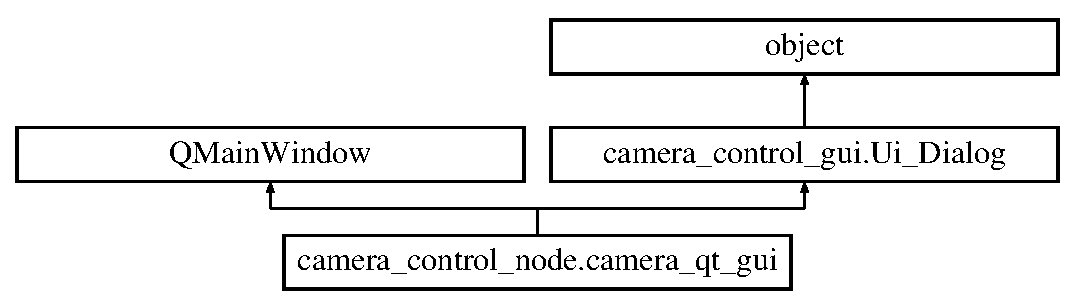
\includegraphics[height=3.000000cm]{classcamera__control__node_1_1camera__qt__gui}
\end{center}
\end{figure}
\subsection*{Classes}
\begin{DoxyCompactItemize}
\item 
class \hyperlink{classcamera__control__node_1_1camera__qt__gui_1_1MODE}{M\-O\-D\-E}
\item 
class \hyperlink{classcamera__control__node_1_1camera__qt__gui_1_1node__name}{node\-\_\-name}
\item 
class \hyperlink{classcamera__control__node_1_1camera__qt__gui_1_1run__dvrk__console}{run\-\_\-dvrk\-\_\-console}
\item 
class \hyperlink{classcamera__control__node_1_1camera__qt__gui_1_1thread__autocamera}{thread\-\_\-autocamera}
\item 
class \hyperlink{classcamera__control__node_1_1camera__qt__gui_1_1thread__bag__writer}{thread\-\_\-bag\-\_\-writer}
\item 
class \hyperlink{classcamera__control__node_1_1camera__qt__gui_1_1thread__clutchNGo}{thread\-\_\-clutch\-N\-Go}
\item 
class \hyperlink{classcamera__control__node_1_1camera__qt__gui_1_1thread__home__arms}{thread\-\_\-home\-\_\-arms}
\item 
class \hyperlink{classcamera__control__node_1_1camera__qt__gui_1_1thread__joystick}{thread\-\_\-joystick}
\item 
class \hyperlink{classcamera__control__node_1_1camera__qt__gui_1_1thread__oculus}{thread\-\_\-oculus}
\item 
class \hyperlink{classcamera__control__node_1_1camera__qt__gui_1_1thread__teleop}{thread\-\_\-teleop}
\item 
class \hyperlink{classcamera__control__node_1_1camera__qt__gui_1_1thread__timer}{thread\-\_\-timer}
\end{DoxyCompactItemize}
\subsection*{Public Member Functions}
\begin{DoxyCompactItemize}
\item 
\hypertarget{classcamera__control__node_1_1camera__qt__gui_a350dfd3a311c4eb1356d947a19243f88}{def {\bfseries \-\_\-\-\_\-init\-\_\-\-\_\-}}\label{classcamera__control__node_1_1camera__qt__gui_a350dfd3a311c4eb1356d947a19243f88}

\item 
\hypertarget{classcamera__control__node_1_1camera__qt__gui_a1943f3510cb4c6a190c5d564c454b01c}{def {\bfseries on\-\_\-record}}\label{classcamera__control__node_1_1camera__qt__gui_a1943f3510cb4c6a190c5d564c454b01c}

\item 
\hypertarget{classcamera__control__node_1_1camera__qt__gui_ae7e563e597e1108f83796b391350af23}{def {\bfseries update\-\_\-timer}}\label{classcamera__control__node_1_1camera__qt__gui_ae7e563e597e1108f83796b391350af23}

\item 
\hypertarget{classcamera__control__node_1_1camera__qt__gui_acf9e10f0ca151297fd527bd78b7eb39e}{def {\bfseries horizontal\-Slider\-Innerzone\-Cb}}\label{classcamera__control__node_1_1camera__qt__gui_acf9e10f0ca151297fd527bd78b7eb39e}

\item 
\hypertarget{classcamera__control__node_1_1camera__qt__gui_a8326bd2fd3ab65f6159d98dda371f6fd}{def {\bfseries horizontal\-Slider\-Deadzone\-Cb}}\label{classcamera__control__node_1_1camera__qt__gui_a8326bd2fd3ab65f6159d98dda371f6fd}

\item 
\hypertarget{classcamera__control__node_1_1camera__qt__gui_a5a6d1330ec073d01cb292de52addbabe}{def {\bfseries set\-\_\-autocamera\-\_\-params}}\label{classcamera__control__node_1_1camera__qt__gui_a5a6d1330ec073d01cb292de52addbabe}

\item 
\hypertarget{classcamera__control__node_1_1camera__qt__gui_ade67a0874337039d0704a444897435b6}{def {\bfseries get\-\_\-autocamera\-\_\-params}}\label{classcamera__control__node_1_1camera__qt__gui_ade67a0874337039d0704a444897435b6}

\item 
\hypertarget{classcamera__control__node_1_1camera__qt__gui_a017df1532a7fd3e7e488083705f502b4}{def {\bfseries home}}\label{classcamera__control__node_1_1camera__qt__gui_a017df1532a7fd3e7e488083705f502b4}

\item 
\hypertarget{classcamera__control__node_1_1camera__qt__gui_a968f68dc23600acfd3f8d5e611e20861}{def {\bfseries power\-\_\-on}}\label{classcamera__control__node_1_1camera__qt__gui_a968f68dc23600acfd3f8d5e611e20861}

\item 
\hypertarget{classcamera__control__node_1_1camera__qt__gui_adde146e4518c7eca00cac6c95e2cb597}{def {\bfseries power\-\_\-off}}\label{classcamera__control__node_1_1camera__qt__gui_adde146e4518c7eca00cac6c95e2cb597}

\item 
\hypertarget{classcamera__control__node_1_1camera__qt__gui_a390a31b5bb49dc30a0b7a53fd99dd9c4}{def {\bfseries reset}}\label{classcamera__control__node_1_1camera__qt__gui_a390a31b5bb49dc30a0b7a53fd99dd9c4}

\item 
\hypertarget{classcamera__control__node_1_1camera__qt__gui_a307b43019be0cc03bbb58eb2354ff478}{def {\bfseries exit\-\_\-program}}\label{classcamera__control__node_1_1camera__qt__gui_a307b43019be0cc03bbb58eb2354ff478}

\item 
\hypertarget{classcamera__control__node_1_1camera__qt__gui_a3ca2db8926ead47cc243825f8e3ea2a0}{def {\bfseries on\-\_\-teleop\-\_\-select}}\label{classcamera__control__node_1_1camera__qt__gui_a3ca2db8926ead47cc243825f8e3ea2a0}

\item 
\hypertarget{classcamera__control__node_1_1camera__qt__gui_a5d787c3893f264df0596b96837688c84}{def {\bfseries on\-\_\-autocamera\-\_\-select}}\label{classcamera__control__node_1_1camera__qt__gui_a5d787c3893f264df0596b96837688c84}

\item 
\hypertarget{classcamera__control__node_1_1camera__qt__gui_ad34134a2d802cf0f34f7ba62b3c652b9}{def {\bfseries on\-\_\-clutch\-N\-Go\-\_\-select}}\label{classcamera__control__node_1_1camera__qt__gui_ad34134a2d802cf0f34f7ba62b3c652b9}

\item 
\hypertarget{classcamera__control__node_1_1camera__qt__gui_a4ceb6ce39f957bca67d6cf749a5c0e36}{def {\bfseries on\-\_\-joystick\-\_\-select}}\label{classcamera__control__node_1_1camera__qt__gui_a4ceb6ce39f957bca67d6cf749a5c0e36}

\item 
\hypertarget{classcamera__control__node_1_1camera__qt__gui_a10eceb42c75d1bfd80c58d04382d3d99}{def {\bfseries on\-\_\-oculus\-\_\-select}}\label{classcamera__control__node_1_1camera__qt__gui_a10eceb42c75d1bfd80c58d04382d3d99}

\item 
\hypertarget{classcamera__control__node_1_1camera__qt__gui_a0d80a2b88d6bcca1b33c525da9985796}{def {\bfseries on\-\_\-simulation\-\_\-select}}\label{classcamera__control__node_1_1camera__qt__gui_a0d80a2b88d6bcca1b33c525da9985796}

\item 
\hypertarget{classcamera__control__node_1_1camera__qt__gui_ae3b93d2ea240bbbbad2de650edac9861}{def {\bfseries on\-\_\-hardware\-\_\-select}}\label{classcamera__control__node_1_1camera__qt__gui_ae3b93d2ea240bbbbad2de650edac9861}

\item 
\hypertarget{classcamera__control__node_1_1camera__qt__gui_a872ea4cb18e184bec92854f1311d6920}{def {\bfseries start\-\_\-node\-\_\-handler}}\label{classcamera__control__node_1_1camera__qt__gui_a872ea4cb18e184bec92854f1311d6920}

\end{DoxyCompactItemize}
\subsection*{Public Attributes}
\begin{DoxyCompactItemize}
\item 
\hypertarget{classcamera__control__node_1_1camera__qt__gui_aa51b652c0ce955aa1eab171ace12a34f}{{\bfseries thread}}\label{classcamera__control__node_1_1camera__qt__gui_aa51b652c0ce955aa1eab171ace12a34f}

\item 
\hypertarget{classcamera__control__node_1_1camera__qt__gui_a17ec8597b564c1546393647b90042168}{{\bfseries thread\-\_\-tel}}\label{classcamera__control__node_1_1camera__qt__gui_a17ec8597b564c1546393647b90042168}

\item 
\hypertarget{classcamera__control__node_1_1camera__qt__gui_ab38ef72cea850f55642e0df46d8245a6}{{\bfseries homing\-\_\-thread}}\label{classcamera__control__node_1_1camera__qt__gui_ab38ef72cea850f55642e0df46d8245a6}

\item 
\hypertarget{classcamera__control__node_1_1camera__qt__gui_acda3362c5fab51e71b724e46f47a869f}{{\bfseries recording}}\label{classcamera__control__node_1_1camera__qt__gui_acda3362c5fab51e71b724e46f47a869f}

\item 
\hypertarget{classcamera__control__node_1_1camera__qt__gui_a94aefe6248a7dd86623facecb9119a2c}{{\bfseries config}}\label{classcamera__control__node_1_1camera__qt__gui_a94aefe6248a7dd86623facecb9119a2c}

\item 
\hypertarget{classcamera__control__node_1_1camera__qt__gui_a314fae61303396fc529a517d6dcce73b}{{\bfseries config\-\_\-file}}\label{classcamera__control__node_1_1camera__qt__gui_a314fae61303396fc529a517d6dcce73b}

\item 
\hypertarget{classcamera__control__node_1_1camera__qt__gui_a17f826b0fd016987d92584d893625d21}{{\bfseries recording\-\_\-dir}}\label{classcamera__control__node_1_1camera__qt__gui_a17f826b0fd016987d92584d893625d21}

\item 
\hypertarget{classcamera__control__node_1_1camera__qt__gui_a5f8f10df5df3319f55c277b824fe29bb}{{\bfseries bag\-\_\-writer}}\label{classcamera__control__node_1_1camera__qt__gui_a5f8f10df5df3319f55c277b824fe29bb}

\item 
\hypertarget{classcamera__control__node_1_1camera__qt__gui_aa8778019630030aa94f283afbe73a036}{{\bfseries recording\-\_\-start\-\_\-time}}\label{classcamera__control__node_1_1camera__qt__gui_aa8778019630030aa94f283afbe73a036}

\item 
\hypertarget{classcamera__control__node_1_1camera__qt__gui_a0a96a70b0345324b47e4f75ec8d5c8a1}{{\bfseries timer\-\_\-thread}}\label{classcamera__control__node_1_1camera__qt__gui_a0a96a70b0345324b47e4f75ec8d5c8a1}

\end{DoxyCompactItemize}


The documentation for this class was generated from the following file\-:\begin{DoxyCompactItemize}
\item 
camera\-\_\-control\-\_\-node.\-py\end{DoxyCompactItemize}

\hypertarget{classclutch__move_1_1ClutchControl}{\section{clutch\-\_\-move.\-Clutch\-Control Class Reference}
\label{classclutch__move_1_1ClutchControl}\index{clutch\-\_\-move.\-Clutch\-Control@{clutch\-\_\-move.\-Clutch\-Control}}
}
\subsection*{Classes}
\begin{DoxyCompactItemize}
\item 
class \hyperlink{classclutch__move_1_1ClutchControl_1_1MODE}{M\-O\-D\-E}
\end{DoxyCompactItemize}
\subsection*{Public Member Functions}
\begin{DoxyCompactItemize}
\item 
\hypertarget{classclutch__move_1_1ClutchControl_a78821936aaca71feb1ac9b5a572e460a}{def {\bfseries \-\_\-\-\_\-init\-\_\-\-\_\-}}\label{classclutch__move_1_1ClutchControl_a78821936aaca71feb1ac9b5a572e460a}

\item 
\hypertarget{classclutch__move_1_1ClutchControl_ad19886b96239b7a02421d6f1cc5d1a46}{def {\bfseries \-\_\-\-\_\-init\-\_\-nodes\-\_\-\-\_\-}}\label{classclutch__move_1_1ClutchControl_ad19886b96239b7a02421d6f1cc5d1a46}

\item 
\hypertarget{classclutch__move_1_1ClutchControl_afa16951229ee2593ac8c20d4c2fe0932}{def {\bfseries shutdown}}\label{classclutch__move_1_1ClutchControl_afa16951229ee2593ac8c20d4c2fe0932}

\item 
def \hyperlink{classclutch__move_1_1ClutchControl_adeec90f2b885e9eb7fa0996905946fa6}{set\-\_\-mode}
\item 
\hypertarget{classclutch__move_1_1ClutchControl_a7331f40df5f951ecdb4f73003a621c08}{def {\bfseries spin}}\label{classclutch__move_1_1ClutchControl_a7331f40df5f951ecdb4f73003a621c08}

\item 
\hypertarget{classclutch__move_1_1ClutchControl_aeb1f6be05fb8375b87d94c15b8f54ec2}{def {\bfseries mtml\-\_\-joint\-\_\-angles\-\_\-cb}}\label{classclutch__move_1_1ClutchControl_aeb1f6be05fb8375b87d94c15b8f54ec2}

\item 
\hypertarget{classclutch__move_1_1ClutchControl_a921610d7970483cf179bfcd57e112d04}{def {\bfseries mtmr\-\_\-joint\-\_\-angles\-\_\-cb}}\label{classclutch__move_1_1ClutchControl_a921610d7970483cf179bfcd57e112d04}

\item 
\hypertarget{classclutch__move_1_1ClutchControl_a9e47180d6e8f1ab29af5b72b5ad1accd}{def {\bfseries psm1\-\_\-joint\-\_\-angles\-\_\-cb}}\label{classclutch__move_1_1ClutchControl_a9e47180d6e8f1ab29af5b72b5ad1accd}

\item 
\hypertarget{classclutch__move_1_1ClutchControl_af72eb5c42ad456aa67c72d874c285b30}{def {\bfseries psm2\-\_\-joint\-\_\-angles\-\_\-cb}}\label{classclutch__move_1_1ClutchControl_af72eb5c42ad456aa67c72d874c285b30}

\item 
\hypertarget{classclutch__move_1_1ClutchControl_a918c26324ce4aa802a407f6c48d5a883}{def {\bfseries mtml\-\_\-cb}}\label{classclutch__move_1_1ClutchControl_a918c26324ce4aa802a407f6c48d5a883}

\item 
\hypertarget{classclutch__move_1_1ClutchControl_abb2c814f27c8b18a12799c42e0caa29a}{def {\bfseries mtmr\-\_\-cb}}\label{classclutch__move_1_1ClutchControl_abb2c814f27c8b18a12799c42e0caa29a}

\item 
\hypertarget{classclutch__move_1_1ClutchControl_a6df92f8f0a444889f4e57019361541c3}{def {\bfseries move\-\_\-mtm\-\_\-out\-\_\-of\-\_\-the\-\_\-way}}\label{classclutch__move_1_1ClutchControl_a6df92f8f0a444889f4e57019361541c3}

\item 
\hypertarget{classclutch__move_1_1ClutchControl_a71bcf76b563276c82b4315bc610d52a6}{def {\bfseries move\-\_\-mtm\-\_\-centerpoints}}\label{classclutch__move_1_1ClutchControl_a71bcf76b563276c82b4315bc610d52a6}

\item 
\hypertarget{classclutch__move_1_1ClutchControl_a2232874a0a60c21017d3eeff2d1dace2}{def {\bfseries enable\-\_\-teleop}}\label{classclutch__move_1_1ClutchControl_a2232874a0a60c21017d3eeff2d1dace2}

\item 
\hypertarget{classclutch__move_1_1ClutchControl_a536d94f7f720d164c97431dd61726c36}{def {\bfseries disable\-\_\-teleop}}\label{classclutch__move_1_1ClutchControl_a536d94f7f720d164c97431dd61726c36}

\item 
\hypertarget{classclutch__move_1_1ClutchControl_aac2e4d4bb322166f9fab90cfc2ccb7ea}{def {\bfseries camera\-\_\-headsensor\-\_\-cb}}\label{classclutch__move_1_1ClutchControl_aac2e4d4bb322166f9fab90cfc2ccb7ea}

\item 
\hypertarget{classclutch__move_1_1ClutchControl_a59754efe91bde7eaafc0dc7139ee40c9}{def {\bfseries camera\-\_\-clutch\-\_\-cb}}\label{classclutch__move_1_1ClutchControl_a59754efe91bde7eaafc0dc7139ee40c9}

\item 
\hypertarget{classclutch__move_1_1ClutchControl_af4f8e0f65b4742c284deff954de64447}{def {\bfseries ecm\-\_\-cb}}\label{classclutch__move_1_1ClutchControl_af4f8e0f65b4742c284deff954de64447}

\item 
\hypertarget{classclutch__move_1_1ClutchControl_a850f1019e440cbb86004426c0ed491b8}{def {\bfseries ecm\-\_\-pan\-\_\-tilt}}\label{classclutch__move_1_1ClutchControl_a850f1019e440cbb86004426c0ed491b8}

\item 
\hypertarget{classclutch__move_1_1ClutchControl_a9f9cbff75e571a9333aebd6d91075751}{def {\bfseries move\-\_\-ecm}}\label{classclutch__move_1_1ClutchControl_a9f9cbff75e571a9333aebd6d91075751}

\item 
\hypertarget{classclutch__move_1_1ClutchControl_a553b9e5c98510b4af1a58c425e6bef09}{def {\bfseries ecm\-\_\-inverse}}\label{classclutch__move_1_1ClutchControl_a553b9e5c98510b4af1a58c425e6bef09}

\item 
\hypertarget{classclutch__move_1_1ClutchControl_afc8847b86a974a3d33dd45783f9e1b29}{def {\bfseries find\-\_\-rotation\-\_\-matrix\-\_\-between\-\_\-two\-\_\-vectors}}\label{classclutch__move_1_1ClutchControl_afc8847b86a974a3d33dd45783f9e1b29}

\end{DoxyCompactItemize}
\subsection*{Public Attributes}
\begin{DoxyCompactItemize}
\item 
\hypertarget{classclutch__move_1_1ClutchControl_a6724145bb091adc282cce8354742e5ab}{{\bfseries camera\-\_\-clutch\-\_\-pressed}}\label{classclutch__move_1_1ClutchControl_a6724145bb091adc282cce8354742e5ab}

\item 
\hypertarget{classclutch__move_1_1ClutchControl_a3b1ceebd5c1b8cb74cf9518bd0ce0c44}{{\bfseries movement\-\_\-scale}}\label{classclutch__move_1_1ClutchControl_a3b1ceebd5c1b8cb74cf9518bd0ce0c44}

\item 
\hypertarget{classclutch__move_1_1ClutchControl_a71a59bdb1fc890de3ed59c7f116d38cf}{{\bfseries joint\-\_\-angles}}\label{classclutch__move_1_1ClutchControl_a71a59bdb1fc890de3ed59c7f116d38cf}

\item 
\hypertarget{classclutch__move_1_1ClutchControl_ad09efab224802cceb80ca62772f32b45}{{\bfseries center}}\label{classclutch__move_1_1ClutchControl_ad09efab224802cceb80ca62772f32b45}

\item 
\hypertarget{classclutch__move_1_1ClutchControl_a8757976c9f476d3a41c77432648c84d0}{{\bfseries flag}}\label{classclutch__move_1_1ClutchControl_a8757976c9f476d3a41c77432648c84d0}

\item 
\hypertarget{classclutch__move_1_1ClutchControl_a97edd4edc499c0b601f1d50e9d28ab83}{{\bfseries mtml\-\_\-pos}}\label{classclutch__move_1_1ClutchControl_a97edd4edc499c0b601f1d50e9d28ab83}

\item 
\hypertarget{classclutch__move_1_1ClutchControl_a47c6e4b1a2e42fe97b54266f182881ad}{{\bfseries mtml\-\_\-joint\-\_\-angles}}\label{classclutch__move_1_1ClutchControl_a47c6e4b1a2e42fe97b54266f182881ad}

\item 
\hypertarget{classclutch__move_1_1ClutchControl_a436eb40b1a4e330d70fd2cddbd0cbe49}{{\bfseries mtmr\-\_\-pos}}\label{classclutch__move_1_1ClutchControl_a436eb40b1a4e330d70fd2cddbd0cbe49}

\item 
\hypertarget{classclutch__move_1_1ClutchControl_a71ca213f571f1f83360fde8e4ef4b82e}{{\bfseries mtmr\-\_\-joint\-\_\-angles}}\label{classclutch__move_1_1ClutchControl_a71ca213f571f1f83360fde8e4ef4b82e}

\item 
\hypertarget{classclutch__move_1_1ClutchControl_ad1bf7d70e87de8c4211452bdc57ca8a4}{{\bfseries mtmr\-\_\-starting\-\_\-point}}\label{classclutch__move_1_1ClutchControl_ad1bf7d70e87de8c4211452bdc57ca8a4}

\item 
\hypertarget{classclutch__move_1_1ClutchControl_afdc7172a845f18f9b565cebdcdb0bce8}{{\bfseries ecm\-\_\-hw}}\label{classclutch__move_1_1ClutchControl_afdc7172a845f18f9b565cebdcdb0bce8}

\item 
\hypertarget{classclutch__move_1_1ClutchControl_a17435a6adb1213a2bc287499513e21f2}{{\bfseries mtmr\-\_\-hw}}\label{classclutch__move_1_1ClutchControl_a17435a6adb1213a2bc287499513e21f2}

\item 
\hypertarget{classclutch__move_1_1ClutchControl_aed24a7359562b84a774f0c14ba338348}{{\bfseries mtml\-\_\-hw}}\label{classclutch__move_1_1ClutchControl_aed24a7359562b84a774f0c14ba338348}

\item 
\hypertarget{classclutch__move_1_1ClutchControl_a68ef45a052ed3dfb6546daad1cabbf20}{{\bfseries mtml\-\_\-hw\-\_\-pub}}\label{classclutch__move_1_1ClutchControl_a68ef45a052ed3dfb6546daad1cabbf20}

\item 
\hypertarget{classclutch__move_1_1ClutchControl_a1864bfc88f5a892faaee4c5096602d0b}{{\bfseries mtmr\-\_\-hw\-\_\-pub}}\label{classclutch__move_1_1ClutchControl_a1864bfc88f5a892faaee4c5096602d0b}

\item 
\hypertarget{classclutch__move_1_1ClutchControl_a1db7f1082676d8e02de955a48c7305a9}{{\bfseries ecm\-\_\-sim}}\label{classclutch__move_1_1ClutchControl_a1db7f1082676d8e02de955a48c7305a9}

\item 
\hypertarget{classclutch__move_1_1ClutchControl_aaa63f07b98d6056c47fcc26ebda232ea}{{\bfseries ecm\-\_\-robot}}\label{classclutch__move_1_1ClutchControl_aaa63f07b98d6056c47fcc26ebda232ea}

\item 
\hypertarget{classclutch__move_1_1ClutchControl_adfbe14818668f283cff25271bb7007b6}{{\bfseries mtmr\-\_\-robot}}\label{classclutch__move_1_1ClutchControl_adfbe14818668f283cff25271bb7007b6}

\item 
\hypertarget{classclutch__move_1_1ClutchControl_a1b6b47b93c96b689f9b6df1a731addb4}{{\bfseries mtml\-\_\-robot}}\label{classclutch__move_1_1ClutchControl_a1b6b47b93c96b689f9b6df1a731addb4}

\item 
\hypertarget{classclutch__move_1_1ClutchControl_a67b712ba92c9d7701cfd18df5ee0fce0}{{\bfseries psm1\-\_\-robot}}\label{classclutch__move_1_1ClutchControl_a67b712ba92c9d7701cfd18df5ee0fce0}

\item 
\hypertarget{classclutch__move_1_1ClutchControl_a98b9f545852d57d20549b8588df916bd}{{\bfseries psm2\-\_\-robot}}\label{classclutch__move_1_1ClutchControl_a98b9f545852d57d20549b8588df916bd}

\item 
\hypertarget{classclutch__move_1_1ClutchControl_a981fe17fd3936a2f889c688fc599d449}{{\bfseries ecm\-\_\-kin}}\label{classclutch__move_1_1ClutchControl_a981fe17fd3936a2f889c688fc599d449}

\item 
\hypertarget{classclutch__move_1_1ClutchControl_af0353e60e4e8e26e6328db7f29523809}{{\bfseries mtmr\-\_\-kin}}\label{classclutch__move_1_1ClutchControl_af0353e60e4e8e26e6328db7f29523809}

\item 
\hypertarget{classclutch__move_1_1ClutchControl_a6684556909abfc6d4ee5acfb4ca45054}{{\bfseries mtml\-\_\-kin}}\label{classclutch__move_1_1ClutchControl_a6684556909abfc6d4ee5acfb4ca45054}

\item 
\hypertarget{classclutch__move_1_1ClutchControl_a85194acaa225df201754d11f8e0aa5c1}{{\bfseries psm1\-\_\-kin}}\label{classclutch__move_1_1ClutchControl_a85194acaa225df201754d11f8e0aa5c1}

\item 
\hypertarget{classclutch__move_1_1ClutchControl_a5bb0a9c255a9cb102e0df8425f2ba3ae}{{\bfseries psm2\-\_\-kin}}\label{classclutch__move_1_1ClutchControl_a5bb0a9c255a9cb102e0df8425f2ba3ae}

\item 
\hypertarget{classclutch__move_1_1ClutchControl_a9f18616fa88f25447d8d6a99619d8258}{{\bfseries mtml\-\_\-orientation}}\label{classclutch__move_1_1ClutchControl_a9f18616fa88f25447d8d6a99619d8258}

\item 
\hypertarget{classclutch__move_1_1ClutchControl_a47d3aa84c1555d4f2c59965d4f6d1855}{{\bfseries mtmr\-\_\-orientation}}\label{classclutch__move_1_1ClutchControl_a47d3aa84c1555d4f2c59965d4f6d1855}

\item 
\hypertarget{classclutch__move_1_1ClutchControl_a95b371e0e4fd8a16ee992a36d9cc274d}{{\bfseries mtml\-\_\-psm2\-\_\-orientation}}\label{classclutch__move_1_1ClutchControl_a95b371e0e4fd8a16ee992a36d9cc274d}

\item 
\hypertarget{classclutch__move_1_1ClutchControl_a07bc6263104b0a29fa043f9bea24ef02}{{\bfseries mtml\-\_\-psm2\-\_\-translation}}\label{classclutch__move_1_1ClutchControl_a07bc6263104b0a29fa043f9bea24ef02}

\item 
\hypertarget{classclutch__move_1_1ClutchControl_a0396b7733e33c0552311ddc9a7b84355}{{\bfseries mtmr\-\_\-psm1\-\_\-orientation}}\label{classclutch__move_1_1ClutchControl_a0396b7733e33c0552311ddc9a7b84355}

\item 
\hypertarget{classclutch__move_1_1ClutchControl_a8cb23f647df80a5915f7bd2058d96891}{{\bfseries mtmr\-\_\-psm1\-\_\-translation}}\label{classclutch__move_1_1ClutchControl_a8cb23f647df80a5915f7bd2058d96891}

\item 
\hypertarget{classclutch__move_1_1ClutchControl_af73204209b6ecea334b0a45eb0dd0b05}{{\bfseries mtmr\-\_\-psm1\-\_\-teleop}}\label{classclutch__move_1_1ClutchControl_af73204209b6ecea334b0a45eb0dd0b05}

\item 
\hypertarget{classclutch__move_1_1ClutchControl_a5c9fe8423625ca03877d42d8a5aeeae0}{{\bfseries mtml\-\_\-psm2\-\_\-teleop}}\label{classclutch__move_1_1ClutchControl_a5c9fe8423625ca03877d42d8a5aeeae0}

\item 
\hypertarget{classclutch__move_1_1ClutchControl_a88ecdafdc5f9032fae4ad1cef94306a6}{{\bfseries sub\-\_\-ecm\-\_\-cb}}\label{classclutch__move_1_1ClutchControl_a88ecdafdc5f9032fae4ad1cef94306a6}

\item 
\hypertarget{classclutch__move_1_1ClutchControl_a90d08eeadef475485ec6b45d40f9024d}{{\bfseries head\-\_\-sensor\-\_\-pressed}}\label{classclutch__move_1_1ClutchControl_a90d08eeadef475485ec6b45d40f9024d}

\item 
\hypertarget{classclutch__move_1_1ClutchControl_ae1b5a2e01d3392b32e923c2f5476f773}{{\bfseries sub\-\_\-camera\-\_\-clutch\-\_\-cb}}\label{classclutch__move_1_1ClutchControl_ae1b5a2e01d3392b32e923c2f5476f773}

\item 
\hypertarget{classclutch__move_1_1ClutchControl_adae170114d8f230b4790dfa2255a2418}{{\bfseries sub\-\_\-headsensor\-\_\-cb}}\label{classclutch__move_1_1ClutchControl_adae170114d8f230b4790dfa2255a2418}

\item 
\hypertarget{classclutch__move_1_1ClutchControl_a39cd7116ac089878994c50c15f203700}{{\bfseries mtml\-\_\-starting\-\_\-point}}\label{classclutch__move_1_1ClutchControl_a39cd7116ac089878994c50c15f203700}

\item 
\hypertarget{classclutch__move_1_1ClutchControl_a3f140caf7bad0a50dc56d2f92c5dd129}{{\bfseries sub\-\_\-mtml\-\_\-cart\-\_\-cb}}\label{classclutch__move_1_1ClutchControl_a3f140caf7bad0a50dc56d2f92c5dd129}

\item 
\hypertarget{classclutch__move_1_1ClutchControl_ae6a760d2454cc5a1f51ef3d6fb1ee1fb}{{\bfseries sub\-\_\-mtml\-\_\-joint\-\_\-cb}}\label{classclutch__move_1_1ClutchControl_ae6a760d2454cc5a1f51ef3d6fb1ee1fb}

\item 
\hypertarget{classclutch__move_1_1ClutchControl_af46c08fb59223ed3a01f7900a3947a92}{{\bfseries sub\-\_\-mtmr\-\_\-cart\-\_\-cb}}\label{classclutch__move_1_1ClutchControl_af46c08fb59223ed3a01f7900a3947a92}

\item 
\hypertarget{classclutch__move_1_1ClutchControl_a4decc04396cd3d78e9c261e24a4ea693}{{\bfseries sub\-\_\-mtmr\-\_\-joint\-\_\-cb}}\label{classclutch__move_1_1ClutchControl_a4decc04396cd3d78e9c261e24a4ea693}

\item 
\hypertarget{classclutch__move_1_1ClutchControl_a4d52341165c93413ec98de524a159e8c}{{\bfseries sub\-\_\-psm1\-\_\-joint\-\_\-cb}}\label{classclutch__move_1_1ClutchControl_a4d52341165c93413ec98de524a159e8c}

\item 
\hypertarget{classclutch__move_1_1ClutchControl_abd7ae3e1ddfe936812cbfb228a638037}{{\bfseries sub\-\_\-psm2\-\_\-joint\-\_\-cb}}\label{classclutch__move_1_1ClutchControl_abd7ae3e1ddfe936812cbfb228a638037}

\item 
\hypertarget{classclutch__move_1_1ClutchControl_a9f80d53cdb7909dcaf732c0d7ca3a1f2}{{\bfseries psm1\-\_\-joint\-\_\-angles}}\label{classclutch__move_1_1ClutchControl_a9f80d53cdb7909dcaf732c0d7ca3a1f2}

\item 
\hypertarget{classclutch__move_1_1ClutchControl_afb1108061df69bc63f90952280770a13}{{\bfseries psm2\-\_\-joint\-\_\-angles}}\label{classclutch__move_1_1ClutchControl_afb1108061df69bc63f90952280770a13}

\item 
\hypertarget{classclutch__move_1_1ClutchControl_aabab35869d417383822d0f026bef43c0}{{\bfseries mtml\-\_\-pos\-\_\-before\-\_\-clutch}}\label{classclutch__move_1_1ClutchControl_aabab35869d417383822d0f026bef43c0}

\item 
\hypertarget{classclutch__move_1_1ClutchControl_ab3bce6cbaeb660bd4dcd220dd7eb5d09}{{\bfseries mtmr\-\_\-pos\-\_\-before\-\_\-clutch}}\label{classclutch__move_1_1ClutchControl_ab3bce6cbaeb660bd4dcd220dd7eb5d09}

\item 
\hypertarget{classclutch__move_1_1ClutchControl_a7bfbc5d68a7d0160b2d65a48b59f6105}{{\bfseries center\-\_\-cart}}\label{classclutch__move_1_1ClutchControl_a7bfbc5d68a7d0160b2d65a48b59f6105}

\end{DoxyCompactItemize}


\subsection{Member Function Documentation}
\hypertarget{classclutch__move_1_1ClutchControl_adeec90f2b885e9eb7fa0996905946fa6}{\index{clutch\-\_\-move\-::\-Clutch\-Control@{clutch\-\_\-move\-::\-Clutch\-Control}!set\-\_\-mode@{set\-\_\-mode}}
\index{set\-\_\-mode@{set\-\_\-mode}!clutch_move::ClutchControl@{clutch\-\_\-move\-::\-Clutch\-Control}}
\subsubsection[{set\-\_\-mode}]{\setlength{\rightskip}{0pt plus 5cm}def clutch\-\_\-move.\-Clutch\-Control.\-set\-\_\-mode (
\begin{DoxyParamCaption}
\item[{}]{self, }
\item[{}]{mode}
\end{DoxyParamCaption}
)}}\label{classclutch__move_1_1ClutchControl_adeec90f2b885e9eb7fa0996905946fa6}
\begin{DoxyVerb}Values:
    MODE.simulation
    MODE.hardware
\end{DoxyVerb}
 

The documentation for this class was generated from the following file\-:\begin{DoxyCompactItemize}
\item 
clutch\-\_\-move.\-py\end{DoxyCompactItemize}

\hypertarget{classcamera__control__node_1_1ClutchControl}{\section{camera\-\_\-control\-\_\-node.\-Clutch\-Control Class Reference}
\label{classcamera__control__node_1_1ClutchControl}\index{camera\-\_\-control\-\_\-node.\-Clutch\-Control@{camera\-\_\-control\-\_\-node.\-Clutch\-Control}}
}
\subsection*{Classes}
\begin{DoxyCompactItemize}
\item 
class \hyperlink{classcamera__control__node_1_1ClutchControl_1_1MODE}{M\-O\-D\-E}
\end{DoxyCompactItemize}
\subsection*{Public Member Functions}
\begin{DoxyCompactItemize}
\item 
\hypertarget{classcamera__control__node_1_1ClutchControl_a329ec738b20b42ee63fc6c0e50c0aec9}{def {\bfseries \-\_\-\-\_\-init\-\_\-\-\_\-}}\label{classcamera__control__node_1_1ClutchControl_a329ec738b20b42ee63fc6c0e50c0aec9}

\item 
\hypertarget{classcamera__control__node_1_1ClutchControl_a2eaba1eb89de4f4189f461cec9287fed}{def {\bfseries \-\_\-\-\_\-init\-\_\-nodes\-\_\-\-\_\-}}\label{classcamera__control__node_1_1ClutchControl_a2eaba1eb89de4f4189f461cec9287fed}

\item 
\hypertarget{classcamera__control__node_1_1ClutchControl_a20cd96e63d4f300e4f01f1dc4bf262f5}{def {\bfseries shutdown}}\label{classcamera__control__node_1_1ClutchControl_a20cd96e63d4f300e4f01f1dc4bf262f5}

\item 
\hypertarget{classcamera__control__node_1_1ClutchControl_a1d68c26ba090afa32862efeb1c13633f}{def {\bfseries set\-\_\-scale}}\label{classcamera__control__node_1_1ClutchControl_a1d68c26ba090afa32862efeb1c13633f}

\item 
def \hyperlink{classcamera__control__node_1_1ClutchControl_adb22cc2cdad0d9eeb9177fd4fb7f39c0}{set\-\_\-mode}
\item 
\hypertarget{classcamera__control__node_1_1ClutchControl_aeccde7deb30d2818014091d903903e88}{def {\bfseries spin}}\label{classcamera__control__node_1_1ClutchControl_aeccde7deb30d2818014091d903903e88}

\item 
\hypertarget{classcamera__control__node_1_1ClutchControl_a6aa54261afbfa7cfd2db59eb0603e87f}{def {\bfseries mtml\-\_\-joint\-\_\-angles\-\_\-cb}}\label{classcamera__control__node_1_1ClutchControl_a6aa54261afbfa7cfd2db59eb0603e87f}

\item 
\hypertarget{classcamera__control__node_1_1ClutchControl_ab436fd936d2dd3a001a019cd1b75b293}{def {\bfseries mtmr\-\_\-joint\-\_\-angles\-\_\-cb}}\label{classcamera__control__node_1_1ClutchControl_ab436fd936d2dd3a001a019cd1b75b293}

\item 
\hypertarget{classcamera__control__node_1_1ClutchControl_a9258ccc6609bd2d0bed2e5dd0daef592}{def {\bfseries psm1\-\_\-joint\-\_\-angles\-\_\-cb}}\label{classcamera__control__node_1_1ClutchControl_a9258ccc6609bd2d0bed2e5dd0daef592}

\item 
\hypertarget{classcamera__control__node_1_1ClutchControl_a29a6b9b5077c633947847fc8eb167a9c}{def {\bfseries psm2\-\_\-joint\-\_\-angles\-\_\-cb}}\label{classcamera__control__node_1_1ClutchControl_a29a6b9b5077c633947847fc8eb167a9c}

\item 
\hypertarget{classcamera__control__node_1_1ClutchControl_a0a94eb2a14c52dd7a6d019d793fe301c}{def {\bfseries \-\_\-\-\_\-mtml\-\_\-cb\-\_\-\-\_\-}}\label{classcamera__control__node_1_1ClutchControl_a0a94eb2a14c52dd7a6d019d793fe301c}

\item 
\hypertarget{classcamera__control__node_1_1ClutchControl_adb59dee096f152db81e3d954ae7c4d0a}{def {\bfseries \-\_\-\-\_\-mtmr\-\_\-cb\-\_\-\-\_\-}}\label{classcamera__control__node_1_1ClutchControl_adb59dee096f152db81e3d954ae7c4d0a}

\item 
\hypertarget{classcamera__control__node_1_1ClutchControl_a833c160e2b110791cdcd5a7eae338b73}{def {\bfseries move\-\_\-mtm\-\_\-centerpoints}}\label{classcamera__control__node_1_1ClutchControl_a833c160e2b110791cdcd5a7eae338b73}

\item 
\hypertarget{classcamera__control__node_1_1ClutchControl_a7912defb689f02008e9c199aa5566250}{def {\bfseries enable\-\_\-teleop}}\label{classcamera__control__node_1_1ClutchControl_a7912defb689f02008e9c199aa5566250}

\item 
\hypertarget{classcamera__control__node_1_1ClutchControl_a309a4d0d285c9440abb99356c70ba59e}{def {\bfseries disable\-\_\-teleop}}\label{classcamera__control__node_1_1ClutchControl_a309a4d0d285c9440abb99356c70ba59e}

\item 
\hypertarget{classcamera__control__node_1_1ClutchControl_acc8234834391215862225d1309ff703a}{def {\bfseries \-\_\-\-\_\-headsensor\-\_\-cb\-\_\-\-\_\-}}\label{classcamera__control__node_1_1ClutchControl_acc8234834391215862225d1309ff703a}

\item 
\hypertarget{classcamera__control__node_1_1ClutchControl_ab7ff325764b3b083affb06e3ebea3628}{def {\bfseries camera\-\_\-clutch\-\_\-cb}}\label{classcamera__control__node_1_1ClutchControl_ab7ff325764b3b083affb06e3ebea3628}

\item 
\hypertarget{classcamera__control__node_1_1ClutchControl_a60e21458df9cf547aa30b3281a135510}{def {\bfseries \-\_\-\-\_\-ecm\-\_\-cb\-\_\-\-\_\-}}\label{classcamera__control__node_1_1ClutchControl_a60e21458df9cf547aa30b3281a135510}

\item 
\hypertarget{classcamera__control__node_1_1ClutchControl_af0f979f6a21e93396964ecfb89f7628f}{def {\bfseries ecm\-\_\-pan\-\_\-tilt}}\label{classcamera__control__node_1_1ClutchControl_af0f979f6a21e93396964ecfb89f7628f}

\item 
\hypertarget{classcamera__control__node_1_1ClutchControl_a615bb82811612d66f58cb3aeacd8e164}{def {\bfseries move\-\_\-ecm}}\label{classcamera__control__node_1_1ClutchControl_a615bb82811612d66f58cb3aeacd8e164}

\item 
\hypertarget{classcamera__control__node_1_1ClutchControl_ae4fb3d2f4c9cd99cd95892b7e139fb9e}{def {\bfseries ecm\-\_\-inverse}}\label{classcamera__control__node_1_1ClutchControl_ae4fb3d2f4c9cd99cd95892b7e139fb9e}

\item 
\hypertarget{classcamera__control__node_1_1ClutchControl_a62a012ce632e5fdb4f6764eeee09826b}{def {\bfseries find\-\_\-rotation\-\_\-matrix\-\_\-between\-\_\-two\-\_\-vectors}}\label{classcamera__control__node_1_1ClutchControl_a62a012ce632e5fdb4f6764eeee09826b}

\end{DoxyCompactItemize}
\subsection*{Public Attributes}
\begin{DoxyCompactItemize}
\item 
\hypertarget{classcamera__control__node_1_1ClutchControl_a0b57d36ee89127df2416a95b36da575f}{{\bfseries teleop\-\_\-thread}}\label{classcamera__control__node_1_1ClutchControl_a0b57d36ee89127df2416a95b36da575f}

\item 
\hypertarget{classcamera__control__node_1_1ClutchControl_a11c7322ef0a3d546f62c2692822c3d39}{{\bfseries camera\-\_\-clutch\-\_\-pressed}}\label{classcamera__control__node_1_1ClutchControl_a11c7322ef0a3d546f62c2692822c3d39}

\item 
\hypertarget{classcamera__control__node_1_1ClutchControl_a294ec01d8a0940c7c69551e612317389}{{\bfseries movement\-\_\-scale}}\label{classcamera__control__node_1_1ClutchControl_a294ec01d8a0940c7c69551e612317389}

\item 
\hypertarget{classcamera__control__node_1_1ClutchControl_aebece0660ece26e354b93906284d068a}{{\bfseries joint\-\_\-angles}}\label{classcamera__control__node_1_1ClutchControl_aebece0660ece26e354b93906284d068a}

\item 
\hypertarget{classcamera__control__node_1_1ClutchControl_a0a0f776c3aa948a86829363ff40c7533}{{\bfseries center}}\label{classcamera__control__node_1_1ClutchControl_a0a0f776c3aa948a86829363ff40c7533}

\item 
\hypertarget{classcamera__control__node_1_1ClutchControl_a48cdf7ff79fdf9ac315d96eb754601a7}{{\bfseries flag}}\label{classcamera__control__node_1_1ClutchControl_a48cdf7ff79fdf9ac315d96eb754601a7}

\item 
\hypertarget{classcamera__control__node_1_1ClutchControl_a94374a3f42c8d88a58ff5b1a5304578e}{{\bfseries mtml\-\_\-pos}}\label{classcamera__control__node_1_1ClutchControl_a94374a3f42c8d88a58ff5b1a5304578e}

\item 
\hypertarget{classcamera__control__node_1_1ClutchControl_a1a6f3c676cea45c14e5f504e749c8cc4}{{\bfseries mtml\-\_\-joint\-\_\-angles}}\label{classcamera__control__node_1_1ClutchControl_a1a6f3c676cea45c14e5f504e749c8cc4}

\item 
\hypertarget{classcamera__control__node_1_1ClutchControl_ac47ab62f0cc3b7cf4feb43e264955e5f}{{\bfseries mtmr\-\_\-pos}}\label{classcamera__control__node_1_1ClutchControl_ac47ab62f0cc3b7cf4feb43e264955e5f}

\item 
\hypertarget{classcamera__control__node_1_1ClutchControl_aac1b3cd9c4f368807b10632c8cf0beae}{{\bfseries mtmr\-\_\-joint\-\_\-angles}}\label{classcamera__control__node_1_1ClutchControl_aac1b3cd9c4f368807b10632c8cf0beae}

\item 
\hypertarget{classcamera__control__node_1_1ClutchControl_a3840d9947829c8faac57a35eadf93147}{{\bfseries mtmr\-\_\-starting\-\_\-point}}\label{classcamera__control__node_1_1ClutchControl_a3840d9947829c8faac57a35eadf93147}

\item 
\hypertarget{classcamera__control__node_1_1ClutchControl_a6fe1d7fa0ed502e6a75a13e25ffa284c}{{\bfseries hw\-\_\-ecm}}\label{classcamera__control__node_1_1ClutchControl_a6fe1d7fa0ed502e6a75a13e25ffa284c}

\item 
\hypertarget{classcamera__control__node_1_1ClutchControl_ab37a19131d9c12619c7f8c14bc35339e}{{\bfseries pub\-\_\-mtml\-\_\-hw}}\label{classcamera__control__node_1_1ClutchControl_ab37a19131d9c12619c7f8c14bc35339e}

\item 
\hypertarget{classcamera__control__node_1_1ClutchControl_ac1072476920a3f5b5bb54a706a0fb0fa}{{\bfseries pub\-\_\-mtmr\-\_\-hw}}\label{classcamera__control__node_1_1ClutchControl_ac1072476920a3f5b5bb54a706a0fb0fa}

\item 
\hypertarget{classcamera__control__node_1_1ClutchControl_a9a16e71b6a3c59bc93ab61c793b77a8c}{{\bfseries pub\-\_\-ecm\-\_\-sim}}\label{classcamera__control__node_1_1ClutchControl_a9a16e71b6a3c59bc93ab61c793b77a8c}

\item 
\hypertarget{classcamera__control__node_1_1ClutchControl_ab0666dfc7afe742a300da218d72e1de4}{{\bfseries hw\-\_\-mtml\-\_\-orientation}}\label{classcamera__control__node_1_1ClutchControl_ab0666dfc7afe742a300da218d72e1de4}

\item 
\hypertarget{classcamera__control__node_1_1ClutchControl_a8616246c3ce05761142866816c03026a}{{\bfseries hw\-\_\-mtmr\-\_\-orientation}}\label{classcamera__control__node_1_1ClutchControl_a8616246c3ce05761142866816c03026a}

\item 
\hypertarget{classcamera__control__node_1_1ClutchControl_a694f648773744c75814adb6f2cfc2b72}{{\bfseries sub\-\_\-ecm\-\_\-cb}}\label{classcamera__control__node_1_1ClutchControl_a694f648773744c75814adb6f2cfc2b72}

\item 
\hypertarget{classcamera__control__node_1_1ClutchControl_a5a377142d2c161db52ea1358328e40d6}{{\bfseries head\-\_\-sensor\-\_\-pressed}}\label{classcamera__control__node_1_1ClutchControl_a5a377142d2c161db52ea1358328e40d6}

\item 
\hypertarget{classcamera__control__node_1_1ClutchControl_a7923723eb29d7844aaa6ea6e1a428a90}{{\bfseries sub\-\_\-camera\-\_\-clutch\-\_\-cb}}\label{classcamera__control__node_1_1ClutchControl_a7923723eb29d7844aaa6ea6e1a428a90}

\item 
\hypertarget{classcamera__control__node_1_1ClutchControl_a23fbfecd7d0bb33bb77c7a86a1fe64fd}{{\bfseries mtml\-\_\-starting\-\_\-point}}\label{classcamera__control__node_1_1ClutchControl_a23fbfecd7d0bb33bb77c7a86a1fe64fd}

\item 
\hypertarget{classcamera__control__node_1_1ClutchControl_a04a25ccd03c3c77560f8c58ab71d89c7}{{\bfseries sub\-\_\-mtml\-\_\-cart\-\_\-cb}}\label{classcamera__control__node_1_1ClutchControl_a04a25ccd03c3c77560f8c58ab71d89c7}

\item 
\hypertarget{classcamera__control__node_1_1ClutchControl_a2fab207698f40e4acbfc4c5564959984}{{\bfseries sub\-\_\-mtml\-\_\-joint\-\_\-cb}}\label{classcamera__control__node_1_1ClutchControl_a2fab207698f40e4acbfc4c5564959984}

\item 
\hypertarget{classcamera__control__node_1_1ClutchControl_a0dc05921efddbb9d8aefdf10f7413b48}{{\bfseries sub\-\_\-mtmr\-\_\-cart\-\_\-cb}}\label{classcamera__control__node_1_1ClutchControl_a0dc05921efddbb9d8aefdf10f7413b48}

\item 
\hypertarget{classcamera__control__node_1_1ClutchControl_a49bbfe7cf8f9017bc3bd0801ae0fe958}{{\bfseries sub\-\_\-mtmr\-\_\-joint\-\_\-cb}}\label{classcamera__control__node_1_1ClutchControl_a49bbfe7cf8f9017bc3bd0801ae0fe958}

\item 
\hypertarget{classcamera__control__node_1_1ClutchControl_a1b61aac947fdb67e0af2371bb35c2be7}{{\bfseries sub\-\_\-psm1\-\_\-joint\-\_\-cb}}\label{classcamera__control__node_1_1ClutchControl_a1b61aac947fdb67e0af2371bb35c2be7}

\item 
\hypertarget{classcamera__control__node_1_1ClutchControl_add58c96afa9be85f8635a29e1ee80cee}{{\bfseries sub\-\_\-psm2\-\_\-joint\-\_\-cb}}\label{classcamera__control__node_1_1ClutchControl_add58c96afa9be85f8635a29e1ee80cee}

\item 
\hypertarget{classcamera__control__node_1_1ClutchControl_a775817956628052da11e59810fee7454}{{\bfseries T\-\_\-mtml\-\_\-pos\-\_\-init}}\label{classcamera__control__node_1_1ClutchControl_a775817956628052da11e59810fee7454}

\item 
\hypertarget{classcamera__control__node_1_1ClutchControl_a5d045655c8566af72bb45a0ab1f33364}{{\bfseries T\-\_\-mtmr\-\_\-pos\-\_\-init}}\label{classcamera__control__node_1_1ClutchControl_a5d045655c8566af72bb45a0ab1f33364}

\item 
\hypertarget{classcamera__control__node_1_1ClutchControl_a48222b3b84647370862ba123e9f9a1af}{{\bfseries mtml\-\_\-pos\-\_\-before\-\_\-clutch}}\label{classcamera__control__node_1_1ClutchControl_a48222b3b84647370862ba123e9f9a1af}

\item 
\hypertarget{classcamera__control__node_1_1ClutchControl_a2c6d74f50e159ccf58febb8f64f8ace1}{{\bfseries mtmr\-\_\-pos\-\_\-before\-\_\-clutch}}\label{classcamera__control__node_1_1ClutchControl_a2c6d74f50e159ccf58febb8f64f8ace1}

\item 
\hypertarget{classcamera__control__node_1_1ClutchControl_a188085bbb4e79a03332d683fa2c4ad98}{{\bfseries psm1\-\_\-joint\-\_\-angles}}\label{classcamera__control__node_1_1ClutchControl_a188085bbb4e79a03332d683fa2c4ad98}

\item 
\hypertarget{classcamera__control__node_1_1ClutchControl_a8852091aed5b402c0179b21749e269ca}{{\bfseries psm2\-\_\-joint\-\_\-angles}}\label{classcamera__control__node_1_1ClutchControl_a8852091aed5b402c0179b21749e269ca}

\item 
\hypertarget{classcamera__control__node_1_1ClutchControl_ad67f4de9850ef3831fd63cf2fed78d50}{{\bfseries center\-\_\-cart}}\label{classcamera__control__node_1_1ClutchControl_ad67f4de9850ef3831fd63cf2fed78d50}

\end{DoxyCompactItemize}


\subsection{Member Function Documentation}
\hypertarget{classcamera__control__node_1_1ClutchControl_adb22cc2cdad0d9eeb9177fd4fb7f39c0}{\index{camera\-\_\-control\-\_\-node\-::\-Clutch\-Control@{camera\-\_\-control\-\_\-node\-::\-Clutch\-Control}!set\-\_\-mode@{set\-\_\-mode}}
\index{set\-\_\-mode@{set\-\_\-mode}!camera_control_node::ClutchControl@{camera\-\_\-control\-\_\-node\-::\-Clutch\-Control}}
\subsubsection[{set\-\_\-mode}]{\setlength{\rightskip}{0pt plus 5cm}def camera\-\_\-control\-\_\-node.\-Clutch\-Control.\-set\-\_\-mode (
\begin{DoxyParamCaption}
\item[{}]{self, }
\item[{}]{mode}
\end{DoxyParamCaption}
)}}\label{classcamera__control__node_1_1ClutchControl_adb22cc2cdad0d9eeb9177fd4fb7f39c0}
\begin{DoxyVerb}Values:
    MODE.simulation
    MODE.hardware
\end{DoxyVerb}
 

The documentation for this class was generated from the following file\-:\begin{DoxyCompactItemize}
\item 
camera\-\_\-control\-\_\-node.\-py\end{DoxyCompactItemize}

\hypertarget{classConvertBags_1_1ConvertBags}{\section{Convert\-Bags.\-Convert\-Bags Class Reference}
\label{classConvertBags_1_1ConvertBags}\index{Convert\-Bags.\-Convert\-Bags@{Convert\-Bags.\-Convert\-Bags}}
}
\subsection*{Public Member Functions}
\begin{DoxyCompactItemize}
\item 
\hypertarget{classConvertBags_1_1ConvertBags_a501d26adbcd8cdea5f39a4399b2028f2}{def {\bfseries \-\_\-\-\_\-init\-\_\-\-\_\-}}\label{classConvertBags_1_1ConvertBags_a501d26adbcd8cdea5f39a4399b2028f2}

\item 
\hypertarget{classConvertBags_1_1ConvertBags_a4e6bbda8fc44d575a34df751b9dd4023}{def {\bfseries Compute\-Cartesian}}\label{classConvertBags_1_1ConvertBags_a4e6bbda8fc44d575a34df751b9dd4023}

\item 
\hypertarget{classConvertBags_1_1ConvertBags_a3fd1970eb9b643601f688f77b0932b4c}{def {\bfseries Write\-Cartesian\-File}}\label{classConvertBags_1_1ConvertBags_a3fd1970eb9b643601f688f77b0932b4c}

\item 
\hypertarget{classConvertBags_1_1ConvertBags_a81e4fdd510e7ce2fcaa1631e607e5c2a}{def {\bfseries Write\-Joint\-Angle\-File}}\label{classConvertBags_1_1ConvertBags_a81e4fdd510e7ce2fcaa1631e607e5c2a}

\item 
\hypertarget{classConvertBags_1_1ConvertBags_a94eda7e24673f6c5c7fff44e7a0d05f4}{def {\bfseries Load\-Tensor\-File\-Joint}}\label{classConvertBags_1_1ConvertBags_a94eda7e24673f6c5c7fff44e7a0d05f4}

\item 
\hypertarget{classConvertBags_1_1ConvertBags_a460e1b42816e88abaf7db6f8bb67ef8a}{def {\bfseries Write\-Tensor\-File\-Joint}}\label{classConvertBags_1_1ConvertBags_a460e1b42816e88abaf7db6f8bb67ef8a}

\item 
\hypertarget{classConvertBags_1_1ConvertBags_a214b012176f1d04e100d3ef26288a32b}{def {\bfseries Load\-Tensor\-File\-Cartesian}}\label{classConvertBags_1_1ConvertBags_a214b012176f1d04e100d3ef26288a32b}

\item 
\hypertarget{classConvertBags_1_1ConvertBags_a9e1872614576da67f0cc82803c3a1295}{def {\bfseries Write\-Tensor\-File\-Cartesian}}\label{classConvertBags_1_1ConvertBags_a9e1872614576da67f0cc82803c3a1295}

\end{DoxyCompactItemize}
\subsection*{Public Attributes}
\begin{DoxyCompactItemize}
\item 
\hypertarget{classConvertBags_1_1ConvertBags_a177d6c6e0202fdd591b5ee2fcfbdaf63}{{\bfseries ecm\-\_\-robot}}\label{classConvertBags_1_1ConvertBags_a177d6c6e0202fdd591b5ee2fcfbdaf63}

\item 
\hypertarget{classConvertBags_1_1ConvertBags_abe4f24db75e9b4eb8bd8ac645ac80431}{{\bfseries ecm\-\_\-kin}}\label{classConvertBags_1_1ConvertBags_abe4f24db75e9b4eb8bd8ac645ac80431}

\item 
\hypertarget{classConvertBags_1_1ConvertBags_af32a2085aa5e72cfc9207bc278c88837}{{\bfseries psm1\-\_\-robot}}\label{classConvertBags_1_1ConvertBags_af32a2085aa5e72cfc9207bc278c88837}

\item 
\hypertarget{classConvertBags_1_1ConvertBags_a5d1c3d2a90705c0757e766f240614c7c}{{\bfseries psm1\-\_\-kin}}\label{classConvertBags_1_1ConvertBags_a5d1c3d2a90705c0757e766f240614c7c}

\item 
\hypertarget{classConvertBags_1_1ConvertBags_aab0d8a35de623c7f3b9f49fb669f318c}{{\bfseries psm2\-\_\-robot}}\label{classConvertBags_1_1ConvertBags_aab0d8a35de623c7f3b9f49fb669f318c}

\item 
\hypertarget{classConvertBags_1_1ConvertBags_a4de373a3a9e0d9732c7d8e7d7898bb14}{{\bfseries psm2\-\_\-kin}}\label{classConvertBags_1_1ConvertBags_a4de373a3a9e0d9732c7d8e7d7898bb14}

\end{DoxyCompactItemize}
\subsection*{Static Public Attributes}
\begin{DoxyCompactItemize}
\item 
\hypertarget{classConvertBags_1_1ConvertBags_a285d5e73b6d3ddb248dadb7342ec0134}{list {\bfseries bag\-\_\-file\-\_\-name} = \mbox{[}$\,$\mbox{]}}\label{classConvertBags_1_1ConvertBags_a285d5e73b6d3ddb248dadb7342ec0134}

\item 
\hypertarget{classConvertBags_1_1ConvertBags_afbb97b84df21d7ad91ffd02668e79f0f}{list {\bfseries bag} = \mbox{[}$\,$\mbox{]}}\label{classConvertBags_1_1ConvertBags_afbb97b84df21d7ad91ffd02668e79f0f}

\item 
list {\bfseries topics\-\_\-cartesian}
\item 
\hypertarget{classConvertBags_1_1ConvertBags_a38547d35c95a25ea2bfb2f54eb7442c2}{list {\bfseries topics\-\_\-joint} = \mbox{[}'/dvrk/P\-S\-M1/state\-\_\-joint\-\_\-current', '/dvrk/P\-S\-M2/state\-\_\-joint\-\_\-current', '/dvrk/E\-C\-M/state\-\_\-joint\-\_\-current'\mbox{]}}\label{classConvertBags_1_1ConvertBags_a38547d35c95a25ea2bfb2f54eb7442c2}

\item 
\hypertarget{classConvertBags_1_1ConvertBags_a985ecbb4c19b14384d48c67847744ad0}{string {\bfseries cartesian\-\_\-header} = \char`\"{}xyzabcd\char`\"{}}\label{classConvertBags_1_1ConvertBags_a985ecbb4c19b14384d48c67847744ad0}

\item 
\hypertarget{classConvertBags_1_1ConvertBags_a97debd757cbccee47557d88a3a191944}{string {\bfseries joint\-\_\-header} = \char`\"{}1234567\char`\"{}}\label{classConvertBags_1_1ConvertBags_a97debd757cbccee47557d88a3a191944}

\item 
tuple \hyperlink{classConvertBags_1_1ConvertBags_a2628e3b073f3ab23e352246cef6e7888}{fid} = open(filename, \char`\"{}w\char`\"{})
\begin{DoxyCompactList}\small\item\em Write a tensor flow file of joint angles to a file. \end{DoxyCompactList}\item 
dictionary \hyperlink{classConvertBags_1_1ConvertBags_a615b423c353271da9d8372a2227e6d74}{d} = \{\}
\begin{DoxyCompactList}\small\item\em returns database variable with all the data and a count. \end{DoxyCompactList}\item 
\hypertarget{classConvertBags_1_1ConvertBags_a69351deeda422a856b9613678082bfc1}{tuple {\bfseries count} = self.\-bag.\-get\-\_\-message\-\_\-count(topic)}\label{classConvertBags_1_1ConvertBags_a69351deeda422a856b9613678082bfc1}

\item 
\hypertarget{classConvertBags_1_1ConvertBags_ab06c5a2d2fe5254ad8a1228293bb0c26}{int {\bfseries i} = 0}\label{classConvertBags_1_1ConvertBags_ab06c5a2d2fe5254ad8a1228293bb0c26}

\item 
\hypertarget{classConvertBags_1_1ConvertBags_aa69c3cef5cb668d3460f2dee7efa89ac}{int {\bfseries j} = 0}\label{classConvertBags_1_1ConvertBags_aa69c3cef5cb668d3460f2dee7efa89ac}

\item 
\hypertarget{classConvertBags_1_1ConvertBags_a79df0e68cb3e91c1585dfdb3ef90ccf1}{string {\bfseries s} = \char`\"{}\char`\"{}}\label{classConvertBags_1_1ConvertBags_a79df0e68cb3e91c1585dfdb3ef90ccf1}

\item 
\hypertarget{classConvertBags_1_1ConvertBags_a79df0e68cb3e91c1585dfdb3ef90ccf1}{list {\bfseries s} = s\mbox{[}0\-:-\/1\mbox{]}}\label{classConvertBags_1_1ConvertBags_a79df0e68cb3e91c1585dfdb3ef90ccf1}

\item 
\hypertarget{classConvertBags_1_1ConvertBags_ab6ea1ad1ed0371079ba4138f5b357b68}{tuple {\bfseries count\-\_\-topics} = len(self.\-topics\-\_\-joint)}\label{classConvertBags_1_1ConvertBags_ab6ea1ad1ed0371079ba4138f5b357b68}

\item 
\hypertarget{classConvertBags_1_1ConvertBags_ab26b293858e77e7f25ad88ffa66e64a8}{tuple {\bfseries count\-\_\-items} = len(self.\-joint\-\_\-header)}\label{classConvertBags_1_1ConvertBags_ab26b293858e77e7f25ad88ffa66e64a8}

\item 
\hypertarget{classConvertBags_1_1ConvertBags_a332cce5421a650993b9990439e75d7c7}{string {\bfseries line} = \char`\"{}\char`\"{}}\label{classConvertBags_1_1ConvertBags_a332cce5421a650993b9990439e75d7c7}

\item 
\hypertarget{classConvertBags_1_1ConvertBags_ad10d99afde24d278dc4018444950bb24}{int {\bfseries jcount} = 4}\label{classConvertBags_1_1ConvertBags_ad10d99afde24d278dc4018444950bb24}

\item 
\hypertarget{classConvertBags_1_1ConvertBags_aafeec80611b542bbf676b017c39f8e02}{tuple {\bfseries line} = line+str(data\mbox{[}topic\mbox{]}\mbox{[}i\mbox{]}\mbox{[}j\mbox{]})}\label{classConvertBags_1_1ConvertBags_aafeec80611b542bbf676b017c39f8e02}

\item 
\hypertarget{classConvertBags_1_1ConvertBags_a332cce5421a650993b9990439e75d7c7}{list {\bfseries line} = line\mbox{[}0\-:-\/1\mbox{]}}\label{classConvertBags_1_1ConvertBags_a332cce5421a650993b9990439e75d7c7}

\end{DoxyCompactItemize}


\subsection{Member Data Documentation}
\hypertarget{classConvertBags_1_1ConvertBags_a615b423c353271da9d8372a2227e6d74}{\index{Convert\-Bags\-::\-Convert\-Bags@{Convert\-Bags\-::\-Convert\-Bags}!d@{d}}
\index{d@{d}!ConvertBags::ConvertBags@{Convert\-Bags\-::\-Convert\-Bags}}
\subsubsection[{d}]{\setlength{\rightskip}{0pt plus 5cm}dictionary Convert\-Bags.\-Convert\-Bags.\-d = \{\}\hspace{0.3cm}{\ttfamily [static]}}}\label{classConvertBags_1_1ConvertBags_a615b423c353271da9d8372a2227e6d74}


returns database variable with all the data and a count. 

open bag file\hypertarget{classConvertBags_1_1ConvertBags_a2628e3b073f3ab23e352246cef6e7888}{\index{Convert\-Bags\-::\-Convert\-Bags@{Convert\-Bags\-::\-Convert\-Bags}!fid@{fid}}
\index{fid@{fid}!ConvertBags::ConvertBags@{Convert\-Bags\-::\-Convert\-Bags}}
\subsubsection[{fid}]{\setlength{\rightskip}{0pt plus 5cm}tuple Convert\-Bags.\-Convert\-Bags.\-fid = open(filename, \char`\"{}w\char`\"{})\hspace{0.3cm}{\ttfamily [static]}}}\label{classConvertBags_1_1ConvertBags_a2628e3b073f3ab23e352246cef6e7888}


Write a tensor flow file of joint angles to a file. 

Write a tensor flow file of Cartesian (xyz and quarternions) to a file.\hypertarget{classConvertBags_1_1ConvertBags_a7872a5a4c775b7e9749f639ac111c234}{\index{Convert\-Bags\-::\-Convert\-Bags@{Convert\-Bags\-::\-Convert\-Bags}!topics\-\_\-cartesian@{topics\-\_\-cartesian}}
\index{topics\-\_\-cartesian@{topics\-\_\-cartesian}!ConvertBags::ConvertBags@{Convert\-Bags\-::\-Convert\-Bags}}
\subsubsection[{topics\-\_\-cartesian}]{\setlength{\rightskip}{0pt plus 5cm}list Convert\-Bags.\-Convert\-Bags.\-topics\-\_\-cartesian\hspace{0.3cm}{\ttfamily [static]}}}\label{classConvertBags_1_1ConvertBags_a7872a5a4c775b7e9749f639ac111c234}
{\bfseries Initial value\-:}
\begin{DoxyCode}
1 = [\textcolor{stringliteral}{'/dvrk/PSM1/position\_cartesian\_current'}, 
2             \textcolor{stringliteral}{'/dvrk/PSM2/position\_cartesian\_current'}, \textcolor{stringliteral}{'/dvrk/ECM/position\_cartesian\_current'}]
\end{DoxyCode}


The documentation for this class was generated from the following file\-:\begin{DoxyCompactItemize}
\item 
Convert\-Bags.\-py\end{DoxyCompactItemize}

\hypertarget{classbase__coregistration_1_1coregistrator}{\section{base\-\_\-coregistration.\-coregistrator Class Reference}
\label{classbase__coregistration_1_1coregistrator}\index{base\-\_\-coregistration.\-coregistrator@{base\-\_\-coregistration.\-coregistrator}}
}
\subsection*{Classes}
\begin{DoxyCompactItemize}
\item 
class \hyperlink{classbase__coregistration_1_1coregistrator_1_1REGISTRATION__MODE}{R\-E\-G\-I\-S\-T\-R\-A\-T\-I\-O\-N\-\_\-\-M\-O\-D\-E}
\end{DoxyCompactItemize}
\subsection*{Public Member Functions}
\begin{DoxyCompactItemize}
\item 
\hypertarget{classbase__coregistration_1_1coregistrator_a400583a5e2a033da40b42717df010255}{def {\bfseries \-\_\-\-\_\-init\-\_\-\-\_\-}}\label{classbase__coregistration_1_1coregistrator_a400583a5e2a033da40b42717df010255}

\item 
\hypertarget{classbase__coregistration_1_1coregistrator_a2db4547e816adb28120db452d1694238}{def {\bfseries psm1\-\_\-read\-\_\-cb}}\label{classbase__coregistration_1_1coregistrator_a2db4547e816adb28120db452d1694238}

\item 
\hypertarget{classbase__coregistration_1_1coregistrator_aeb8e5b51da276807ab20cc6fe04e1e7a}{def {\bfseries psm2\-\_\-read\-\_\-cb}}\label{classbase__coregistration_1_1coregistrator_aeb8e5b51da276807ab20cc6fe04e1e7a}

\item 
\hypertarget{classbase__coregistration_1_1coregistrator_afb888ab42c1a09b22565e5433008f255}{def {\bfseries ecm\-\_\-read\-\_\-cb}}\label{classbase__coregistration_1_1coregistrator_afb888ab42c1a09b22565e5433008f255}

\item 
\hypertarget{classbase__coregistration_1_1coregistrator_a5903f36eada18b55a184c5bbd278fca1}{def {\bfseries collect}}\label{classbase__coregistration_1_1coregistrator_a5903f36eada18b55a184c5bbd278fca1}

\item 
\hypertarget{classbase__coregistration_1_1coregistrator_a685597c0479bb157073d3861b9f1a4d4}{def {\bfseries save\-\_\-to\-\_\-db}}\label{classbase__coregistration_1_1coregistrator_a685597c0479bb157073d3861b9f1a4d4}

\item 
\hypertarget{classbase__coregistration_1_1coregistrator_a42fc6242c68378fe0eba9be768a8449f}{def {\bfseries read\-\_\-from\-\_\-db}}\label{classbase__coregistration_1_1coregistrator_a42fc6242c68378fe0eba9be768a8449f}

\item 
\hypertarget{classbase__coregistration_1_1coregistrator_af92c1a10a77d7b73dcfaace696262e3d}{def {\bfseries compute\-\_\-fk}}\label{classbase__coregistration_1_1coregistrator_af92c1a10a77d7b73dcfaace696262e3d}

\item 
\hypertarget{classbase__coregistration_1_1coregistrator_a2821c24de419a9321f1b9002dac779ba}{def {\bfseries dist}}\label{classbase__coregistration_1_1coregistrator_a2821c24de419a9321f1b9002dac779ba}

\item 
\hypertarget{classbase__coregistration_1_1coregistrator_ad625a7fa017378453567d0520897cfd2}{def {\bfseries objective\-\_\-function}}\label{classbase__coregistration_1_1coregistrator_ad625a7fa017378453567d0520897cfd2}

\item 
\hypertarget{classbase__coregistration_1_1coregistrator_ad462b54905e52e5a8b2255a32a64ad78}{def {\bfseries find\-\_\-everything\-\_\-related\-\_\-to\-\_\-world}}\label{classbase__coregistration_1_1coregistrator_ad462b54905e52e5a8b2255a32a64ad78}

\item 
\hypertarget{classbase__coregistration_1_1coregistrator_aad261d9a716de016b37d5da82e63d59b}{def {\bfseries optimize\-\_\-bases}}\label{classbase__coregistration_1_1coregistrator_aad261d9a716de016b37d5da82e63d59b}

\end{DoxyCompactItemize}
\subsection*{Public Attributes}
\begin{DoxyCompactItemize}
\item 
\hypertarget{classbase__coregistration_1_1coregistrator_a8da816f13096f3835b433660bfb45ce8}{{\bfseries psm1\-\_\-robot}}\label{classbase__coregistration_1_1coregistrator_a8da816f13096f3835b433660bfb45ce8}

\item 
\hypertarget{classbase__coregistration_1_1coregistrator_ad2e447a005c1c0e3f30d3d55ba3c0829}{{\bfseries psm1\-\_\-kin}}\label{classbase__coregistration_1_1coregistrator_ad2e447a005c1c0e3f30d3d55ba3c0829}

\item 
\hypertarget{classbase__coregistration_1_1coregistrator_a3a3ae08f5e181df76731b299ef44b573}{{\bfseries psm2\-\_\-robot}}\label{classbase__coregistration_1_1coregistrator_a3a3ae08f5e181df76731b299ef44b573}

\item 
\hypertarget{classbase__coregistration_1_1coregistrator_aaf1e0b3bc308faee6e926fe088b3d592}{{\bfseries psm2\-\_\-kin}}\label{classbase__coregistration_1_1coregistrator_aaf1e0b3bc308faee6e926fe088b3d592}

\item 
\hypertarget{classbase__coregistration_1_1coregistrator_afaf27e8bb632e57ced50a69fa4ce1ead}{{\bfseries ecm\-\_\-robot}}\label{classbase__coregistration_1_1coregistrator_afaf27e8bb632e57ced50a69fa4ce1ead}

\item 
\hypertarget{classbase__coregistration_1_1coregistrator_abd27890240364b7bbf67928e6d89f3cb}{{\bfseries ecm\-\_\-kin}}\label{classbase__coregistration_1_1coregistrator_abd27890240364b7bbf67928e6d89f3cb}

\item 
\hypertarget{classbase__coregistration_1_1coregistrator_a02a6b0d225740b624425863b0019beeb}{{\bfseries psm1\-\_\-read\-\_\-cb\-\_\-save}}\label{classbase__coregistration_1_1coregistrator_a02a6b0d225740b624425863b0019beeb}

\item 
\hypertarget{classbase__coregistration_1_1coregistrator_afcdea4e1436d4e9797e1cb79d596df8f}{{\bfseries psm1\-\_\-read\-\_\-cb\-\_\-count}}\label{classbase__coregistration_1_1coregistrator_afcdea4e1436d4e9797e1cb79d596df8f}

\item 
\hypertarget{classbase__coregistration_1_1coregistrator_ad2374fdab9f79db544fe586860e5efc9}{{\bfseries psm2\-\_\-read\-\_\-cb\-\_\-save}}\label{classbase__coregistration_1_1coregistrator_ad2374fdab9f79db544fe586860e5efc9}

\item 
\hypertarget{classbase__coregistration_1_1coregistrator_a361efaacc34fb50c8eea2d1b149d3653}{{\bfseries psm2\-\_\-read\-\_\-cb\-\_\-count}}\label{classbase__coregistration_1_1coregistrator_a361efaacc34fb50c8eea2d1b149d3653}

\item 
\hypertarget{classbase__coregistration_1_1coregistrator_ae58982e5f9fbafb53cdd372695fd8a7e}{{\bfseries ecm\-\_\-read\-\_\-cb\-\_\-save}}\label{classbase__coregistration_1_1coregistrator_ae58982e5f9fbafb53cdd372695fd8a7e}

\item 
\hypertarget{classbase__coregistration_1_1coregistrator_ace065946b7b2362fb8f4553b34e83ed3}{{\bfseries ecm\-\_\-read\-\_\-cb\-\_\-count}}\label{classbase__coregistration_1_1coregistrator_ace065946b7b2362fb8f4553b34e83ed3}

\item 
\hypertarget{classbase__coregistration_1_1coregistrator_a735ac19f7e3d17739201c74067c1079d}{{\bfseries collected\-\_\-joint\-\_\-angles}}\label{classbase__coregistration_1_1coregistrator_a735ac19f7e3d17739201c74067c1079d}

\end{DoxyCompactItemize}
\subsection*{Static Public Attributes}
\begin{DoxyCompactItemize}
\item 
\hypertarget{classbase__coregistration_1_1coregistrator_ad4c82912da3ced9a97cca6d003cf6ed5}{{\bfseries mode} = R\-E\-G\-I\-S\-T\-R\-A\-T\-I\-O\-N\-\_\-\-M\-O\-D\-E.\-P\-S\-M1\-\_\-\-P\-S\-M2}\label{classbase__coregistration_1_1coregistrator_ad4c82912da3ced9a97cca6d003cf6ed5}

\item 
\hypertarget{classbase__coregistration_1_1coregistrator_abec95ddacfe2df642c94149730f1b160}{{\bfseries psm1\-\_\-data} = None}\label{classbase__coregistration_1_1coregistrator_abec95ddacfe2df642c94149730f1b160}

\item 
\hypertarget{classbase__coregistration_1_1coregistrator_a66efe42e6796f28399b28f99d464670a}{{\bfseries psm2\-\_\-data} = None}\label{classbase__coregistration_1_1coregistrator_a66efe42e6796f28399b28f99d464670a}

\item 
\hypertarget{classbase__coregistration_1_1coregistrator_ab59ae8bc38c01419c91796c922c35540}{{\bfseries ecm\-\_\-data} = None}\label{classbase__coregistration_1_1coregistrator_ab59ae8bc38c01419c91796c922c35540}

\end{DoxyCompactItemize}


\subsection{Detailed Description}
\begin{DoxyVerb}    The coregistrator class collects the joint angles from the da vinci platform and 
    optimizes the relative transformation of their bases. We have to touch the tips 
    of two pairs of arms together and record the data a few times. Then run the 
    optimization algorithm. We need to do it twice one for psm1 and psm2, and another
    one for psm1 and ecm.
\end{DoxyVerb}
 

The documentation for this class was generated from the following file\-:\begin{DoxyCompactItemize}
\item 
base\-\_\-coregistration.\-py\end{DoxyCompactItemize}

\hypertarget{classcontrol__arms_1_1Example}{\section{control\-\_\-arms.\-Example Class Reference}
\label{classcontrol__arms_1_1Example}\index{control\-\_\-arms.\-Example@{control\-\_\-arms.\-Example}}
}
Inheritance diagram for control\-\_\-arms.\-Example\-:\begin{figure}[H]
\begin{center}
\leavevmode
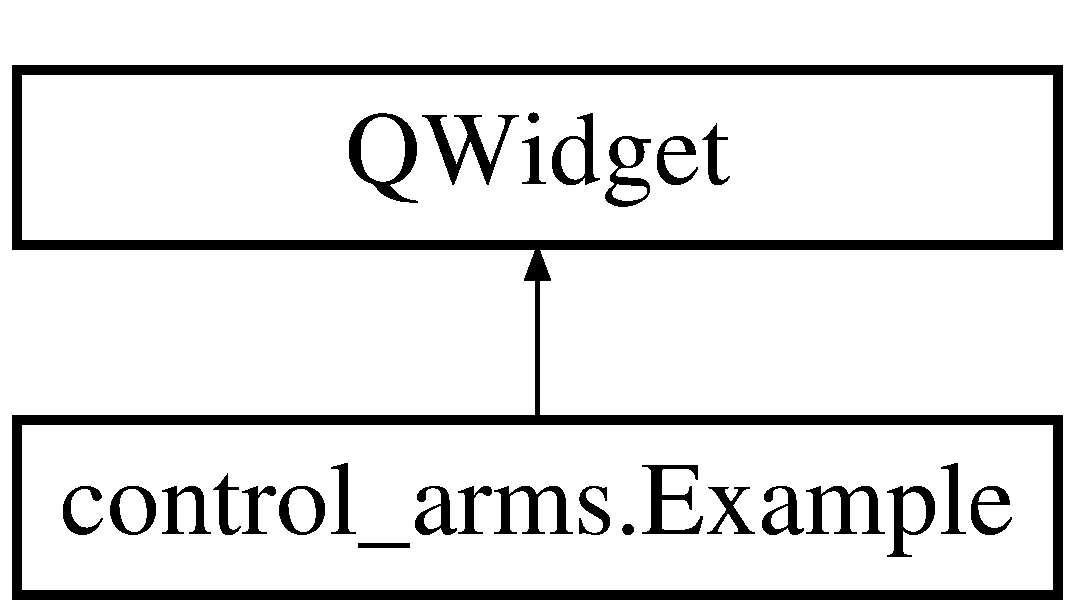
\includegraphics[height=2.000000cm]{classcontrol__arms_1_1Example}
\end{center}
\end{figure}
\subsection*{Public Member Functions}
\begin{DoxyCompactItemize}
\item 
\hypertarget{classcontrol__arms_1_1Example_ad58d2749ddc76efd2f31759852d0befe}{def {\bfseries \-\_\-\-\_\-init\-\_\-\-\_\-}}\label{classcontrol__arms_1_1Example_ad58d2749ddc76efd2f31759852d0befe}

\item 
\hypertarget{classcontrol__arms_1_1Example_a0630b59cab4a2b355b9936ce6163543e}{def {\bfseries init\-U\-I}}\label{classcontrol__arms_1_1Example_a0630b59cab4a2b355b9936ce6163543e}

\item 
\hypertarget{classcontrol__arms_1_1Example_a1564ef7b522ba9664ec7453556092d9c}{def {\bfseries change\-Value0}}\label{classcontrol__arms_1_1Example_a1564ef7b522ba9664ec7453556092d9c}

\item 
\hypertarget{classcontrol__arms_1_1Example_a27a30fa7b4ad54d273d981747d7b4f3a}{def {\bfseries change\-Value1}}\label{classcontrol__arms_1_1Example_a27a30fa7b4ad54d273d981747d7b4f3a}

\item 
\hypertarget{classcontrol__arms_1_1Example_ada953ae89ce86e69f09fbffdecf26933}{def {\bfseries change\-Value2}}\label{classcontrol__arms_1_1Example_ada953ae89ce86e69f09fbffdecf26933}

\item 
\hypertarget{classcontrol__arms_1_1Example_a425878b416e27418671ca20df44638cf}{def {\bfseries change\-Value3}}\label{classcontrol__arms_1_1Example_a425878b416e27418671ca20df44638cf}

\end{DoxyCompactItemize}
\subsection*{Public Attributes}
\begin{DoxyCompactItemize}
\item 
\hypertarget{classcontrol__arms_1_1Example_a8d7538a6cd0eb119cd8d656ddadc2238}{{\bfseries label}}\label{classcontrol__arms_1_1Example_a8d7538a6cd0eb119cd8d656ddadc2238}

\end{DoxyCompactItemize}


The documentation for this class was generated from the following file\-:\begin{DoxyCompactItemize}
\item 
control\-\_\-arms.\-py\end{DoxyCompactItemize}

\hypertarget{classcamera__control__node_1_1Joystick}{\section{camera\-\_\-control\-\_\-node.\-Joystick Class Reference}
\label{classcamera__control__node_1_1Joystick}\index{camera\-\_\-control\-\_\-node.\-Joystick@{camera\-\_\-control\-\_\-node.\-Joystick}}
}
\subsection*{Classes}
\begin{DoxyCompactItemize}
\item 
class \hyperlink{classcamera__control__node_1_1Joystick_1_1MODE}{M\-O\-D\-E}
\end{DoxyCompactItemize}
\subsection*{Public Member Functions}
\begin{DoxyCompactItemize}
\item 
\hypertarget{classcamera__control__node_1_1Joystick_a2ccaafba9a6e2eaa11765ca70e47b450}{def {\bfseries \-\_\-\-\_\-init\-\_\-\-\_\-}}\label{classcamera__control__node_1_1Joystick_a2ccaafba9a6e2eaa11765ca70e47b450}

\item 
\hypertarget{classcamera__control__node_1_1Joystick_a11734fdf511eca3d9161d0f3b21dd8bb}{def {\bfseries \-\_\-\-\_\-init\-\_\-nodes\-\_\-\-\_\-}}\label{classcamera__control__node_1_1Joystick_a11734fdf511eca3d9161d0f3b21dd8bb}

\item 
\hypertarget{classcamera__control__node_1_1Joystick_afc58e3de9c4d4be0329043d3fc8821a8}{def {\bfseries shutdown}}\label{classcamera__control__node_1_1Joystick_afc58e3de9c4d4be0329043d3fc8821a8}

\item 
\hypertarget{classcamera__control__node_1_1Joystick_a65ca6d1fcff05cdb66d859ac6767ca2b}{def {\bfseries set\-\_\-mode}}\label{classcamera__control__node_1_1Joystick_a65ca6d1fcff05cdb66d859ac6767ca2b}

\item 
\hypertarget{classcamera__control__node_1_1Joystick_aed7d82093458cee174ac621ddfdc19d6}{def {\bfseries spin}}\label{classcamera__control__node_1_1Joystick_aed7d82093458cee174ac621ddfdc19d6}

\item 
\hypertarget{classcamera__control__node_1_1Joystick_aca6b799c87890972ef76f98adda07776}{def {\bfseries \-\_\-\-\_\-spin\-\_\-\-\_\-}}\label{classcamera__control__node_1_1Joystick_aca6b799c87890972ef76f98adda07776}

\item 
\hypertarget{classcamera__control__node_1_1Joystick_a6803a241d22f8881c2006df53f81e39b}{def {\bfseries \-\_\-\-\_\-ecm\-\_\-cb\-\_\-\-\_\-}}\label{classcamera__control__node_1_1Joystick_a6803a241d22f8881c2006df53f81e39b}

\item 
\hypertarget{classcamera__control__node_1_1Joystick_aa2b243c6e5174565960a8c9fab5c8735}{def {\bfseries ecm\-\_\-joystick\-\_\-recenter}}\label{classcamera__control__node_1_1Joystick_aa2b243c6e5174565960a8c9fab5c8735}

\item 
\hypertarget{classcamera__control__node_1_1Joystick_af7c7d25e1f510404d1ca686075f0d413}{def {\bfseries on\-\_\-joystick\-\_\-change\-\_\-cb}}\label{classcamera__control__node_1_1Joystick_af7c7d25e1f510404d1ca686075f0d413}

\item 
\hypertarget{classcamera__control__node_1_1Joystick_a4e044503ddaf52beed10a40dc8f7393b}{def {\bfseries ecm\-\_\-zoom}}\label{classcamera__control__node_1_1Joystick_a4e044503ddaf52beed10a40dc8f7393b}

\item 
\hypertarget{classcamera__control__node_1_1Joystick_addaad41efd9c5b295a5ac5292b1ccd58}{def {\bfseries ecm\-\_\-pan\-\_\-tilt}}\label{classcamera__control__node_1_1Joystick_addaad41efd9c5b295a5ac5292b1ccd58}

\item 
\hypertarget{classcamera__control__node_1_1Joystick_addd6b22853ec207c38f4d46c8b4dea8e}{def {\bfseries move\-\_\-ecm}}\label{classcamera__control__node_1_1Joystick_addd6b22853ec207c38f4d46c8b4dea8e}

\item 
\hypertarget{classcamera__control__node_1_1Joystick_a61c5bcd6529c6879a7f9e31ac137dfd3}{def {\bfseries ecm\-\_\-inverse}}\label{classcamera__control__node_1_1Joystick_a61c5bcd6529c6879a7f9e31ac137dfd3}

\item 
\hypertarget{classcamera__control__node_1_1Joystick_a3cae95116ab2d0247069207d0b751ede}{def {\bfseries find\-\_\-rotation\-\_\-matrix\-\_\-between\-\_\-two\-\_\-vectors}}\label{classcamera__control__node_1_1Joystick_a3cae95116ab2d0247069207d0b751ede}

\end{DoxyCompactItemize}
\subsection*{Public Attributes}
\begin{DoxyCompactItemize}
\item 
\hypertarget{classcamera__control__node_1_1Joystick_a2aca30b41163343e4a158f3569fe2c2a}{{\bfseries joint\-\_\-angles}}\label{classcamera__control__node_1_1Joystick_a2aca30b41163343e4a158f3569fe2c2a}

\item 
\hypertarget{classcamera__control__node_1_1Joystick_a962b4d57e9f638349419c2448e1c5d7d}{{\bfseries center}}\label{classcamera__control__node_1_1Joystick_a962b4d57e9f638349419c2448e1c5d7d}

\item 
\hypertarget{classcamera__control__node_1_1Joystick_a79545292813ab5869a4c58b170321101}{{\bfseries joystick\-\_\-at\-\_\-zero}}\label{classcamera__control__node_1_1Joystick_a79545292813ab5869a4c58b170321101}

\item 
\hypertarget{classcamera__control__node_1_1Joystick_afd084eb67b2cb13d88d438164897ff66}{{\bfseries movement\-\_\-scale}}\label{classcamera__control__node_1_1Joystick_afd084eb67b2cb13d88d438164897ff66}

\item 
\hypertarget{classcamera__control__node_1_1Joystick_aa71fd0c6b463c0cf2a56c306a6cb0a79}{{\bfseries last\-\_\-z}}\label{classcamera__control__node_1_1Joystick_aa71fd0c6b463c0cf2a56c306a6cb0a79}

\item 
\hypertarget{classcamera__control__node_1_1Joystick_a2231bbdeebe9bcd5a122d56c12a7dedb}{{\bfseries control\-\_\-mode}}\label{classcamera__control__node_1_1Joystick_a2231bbdeebe9bcd5a122d56c12a7dedb}

\item 
\hypertarget{classcamera__control__node_1_1Joystick_aa04b594fe6dbcf64de563857a7b0f35a}{{\bfseries hw\-\_\-ecm}}\label{classcamera__control__node_1_1Joystick_aa04b594fe6dbcf64de563857a7b0f35a}

\item 
\hypertarget{classcamera__control__node_1_1Joystick_aec2d0dc10f1a4311799abe88db485c02}{{\bfseries pub\-\_\-ecm\-\_\-sim}}\label{classcamera__control__node_1_1Joystick_aec2d0dc10f1a4311799abe88db485c02}

\item 
\hypertarget{classcamera__control__node_1_1Joystick_a107e4d6a790f2bf5fc48e51aec2bbbe4}{{\bfseries sub\-\_\-joy}}\label{classcamera__control__node_1_1Joystick_a107e4d6a790f2bf5fc48e51aec2bbbe4}

\end{DoxyCompactItemize}
\subsection*{Static Public Attributes}
\begin{DoxyCompactItemize}
\item 
\hypertarget{classcamera__control__node_1_1Joystick_aa2795dcb8fee14a8e96937dd5fb7edeb}{string {\bfseries A\-B\-S\-O\-L\-U\-T\-E\-\_\-\-C\-O\-N\-T\-R\-O\-L} = \char`\"{}A\-B\-S\-O\-L\-U\-T\-E\-\_\-\-C\-O\-N\-T\-R\-O\-L\char`\"{}}\label{classcamera__control__node_1_1Joystick_aa2795dcb8fee14a8e96937dd5fb7edeb}

\end{DoxyCompactItemize}


The documentation for this class was generated from the following file\-:\begin{DoxyCompactItemize}
\item 
camera\-\_\-control\-\_\-node.\-py\end{DoxyCompactItemize}

\hypertarget{classjoystick_1_1Joystick}{\section{joystick.\-Joystick Class Reference}
\label{classjoystick_1_1Joystick}\index{joystick.\-Joystick@{joystick.\-Joystick}}
}
\subsection*{Classes}
\begin{DoxyCompactItemize}
\item 
class \hyperlink{classjoystick_1_1Joystick_1_1MODE}{M\-O\-D\-E}
\end{DoxyCompactItemize}
\subsection*{Public Member Functions}
\begin{DoxyCompactItemize}
\item 
\hypertarget{classjoystick_1_1Joystick_afef248a64bb142746b07f4f3af62388d}{def {\bfseries \-\_\-\-\_\-init\-\_\-\-\_\-}}\label{classjoystick_1_1Joystick_afef248a64bb142746b07f4f3af62388d}

\item 
\hypertarget{classjoystick_1_1Joystick_a873b6b966873adb22d8f807fcb5059f3}{def {\bfseries \-\_\-\-\_\-init\-\_\-nodes\-\_\-\-\_\-}}\label{classjoystick_1_1Joystick_a873b6b966873adb22d8f807fcb5059f3}

\item 
\hypertarget{classjoystick_1_1Joystick_a5fc42dd4d953577f4d3033cbe1c4754b}{def {\bfseries \-\_\-\-\_\-spin\-\_\-\-\_\-}}\label{classjoystick_1_1Joystick_a5fc42dd4d953577f4d3033cbe1c4754b}

\item 
\hypertarget{classjoystick_1_1Joystick_a04a9a65f1b7beb59b2d4935dc83dbd63}{def {\bfseries ecm\-\_\-cb}}\label{classjoystick_1_1Joystick_a04a9a65f1b7beb59b2d4935dc83dbd63}

\item 
\hypertarget{classjoystick_1_1Joystick_a644ff07de55168ab4d3fa98b7724b76b}{def {\bfseries ecm\-\_\-joystick\-\_\-recenter}}\label{classjoystick_1_1Joystick_a644ff07de55168ab4d3fa98b7724b76b}

\item 
\hypertarget{classjoystick_1_1Joystick_ad708a220d4c2019749d60a5b34bc904e}{def {\bfseries on\-\_\-joystick\-\_\-change\-\_\-cb}}\label{classjoystick_1_1Joystick_ad708a220d4c2019749d60a5b34bc904e}

\item 
\hypertarget{classjoystick_1_1Joystick_a9a784dbb2800a878a25f87708fae9e07}{def {\bfseries ecm\-\_\-zoom}}\label{classjoystick_1_1Joystick_a9a784dbb2800a878a25f87708fae9e07}

\item 
\hypertarget{classjoystick_1_1Joystick_ab8dddbccfcd5fc508d9607de1b6c6abe}{def {\bfseries ecm\-\_\-pan\-\_\-tilt}}\label{classjoystick_1_1Joystick_ab8dddbccfcd5fc508d9607de1b6c6abe}

\item 
\hypertarget{classjoystick_1_1Joystick_ab6b036728117f78839c836e3b3595b1a}{def {\bfseries move\-\_\-ecm}}\label{classjoystick_1_1Joystick_ab6b036728117f78839c836e3b3595b1a}

\item 
\hypertarget{classjoystick_1_1Joystick_a764b643d59fa789b8dd339c7684facad}{def {\bfseries ecm\-\_\-inverse}}\label{classjoystick_1_1Joystick_a764b643d59fa789b8dd339c7684facad}

\item 
\hypertarget{classjoystick_1_1Joystick_ad8222325ba8fd2900ab5734b8f2c2286}{def {\bfseries find\-\_\-rotation\-\_\-matrix\-\_\-between\-\_\-two\-\_\-vectors}}\label{classjoystick_1_1Joystick_ad8222325ba8fd2900ab5734b8f2c2286}

\end{DoxyCompactItemize}
\subsection*{Public Attributes}
\begin{DoxyCompactItemize}
\item 
\hypertarget{classjoystick_1_1Joystick_a90f93349791a015725873f595d41b76a}{{\bfseries joint\-\_\-angles}}\label{classjoystick_1_1Joystick_a90f93349791a015725873f595d41b76a}

\item 
\hypertarget{classjoystick_1_1Joystick_af68af8c1391522280fddd6089c6a0b43}{{\bfseries center}}\label{classjoystick_1_1Joystick_af68af8c1391522280fddd6089c6a0b43}

\item 
\hypertarget{classjoystick_1_1Joystick_a82bf14720133a3294020554347bf1f5a}{{\bfseries joystick\-\_\-at\-\_\-zero}}\label{classjoystick_1_1Joystick_a82bf14720133a3294020554347bf1f5a}

\item 
\hypertarget{classjoystick_1_1Joystick_a5eaa063fe5b8c7afb634165a0380534b}{{\bfseries movement\-\_\-scale}}\label{classjoystick_1_1Joystick_a5eaa063fe5b8c7afb634165a0380534b}

\item 
\hypertarget{classjoystick_1_1Joystick_a4ecd0948bda8c8154b9ae37de92f24b4}{{\bfseries last\-\_\-z}}\label{classjoystick_1_1Joystick_a4ecd0948bda8c8154b9ae37de92f24b4}

\item 
\hypertarget{classjoystick_1_1Joystick_a38de7a8c2a5b76976462666bc15c3182}{{\bfseries ecm\-\_\-hw}}\label{classjoystick_1_1Joystick_a38de7a8c2a5b76976462666bc15c3182}

\item 
\hypertarget{classjoystick_1_1Joystick_a7892d4ac35c98d63a1bd1187b071eecb}{{\bfseries ecm\-\_\-sim}}\label{classjoystick_1_1Joystick_a7892d4ac35c98d63a1bd1187b071eecb}

\item 
\hypertarget{classjoystick_1_1Joystick_afb2f76d862615a983a9d9d208e83cbb9}{{\bfseries ecm\-\_\-robot}}\label{classjoystick_1_1Joystick_afb2f76d862615a983a9d9d208e83cbb9}

\item 
\hypertarget{classjoystick_1_1Joystick_a842aa6758b92b526ea3d213ea96fb3f0}{{\bfseries ecm\-\_\-kin}}\label{classjoystick_1_1Joystick_a842aa6758b92b526ea3d213ea96fb3f0}

\end{DoxyCompactItemize}


The documentation for this class was generated from the following file\-:\begin{DoxyCompactItemize}
\item 
joystick.\-py\end{DoxyCompactItemize}

\hypertarget{classjoystick_1_1Joystick_1_1MODE}{\section{joystick.\-Joystick.\-M\-O\-D\-E Class Reference}
\label{classjoystick_1_1Joystick_1_1MODE}\index{joystick.\-Joystick.\-M\-O\-D\-E@{joystick.\-Joystick.\-M\-O\-D\-E}}
}
\subsection*{Static Public Attributes}
\begin{DoxyCompactItemize}
\item 
\hypertarget{classjoystick_1_1Joystick_1_1MODE_a3b7c644e67c3db15dd2c665d231c5def}{string {\bfseries simulation} = \char`\"{}S\-I\-M\-U\-L\-A\-T\-I\-O\-N\char`\"{}}\label{classjoystick_1_1Joystick_1_1MODE_a3b7c644e67c3db15dd2c665d231c5def}

\item 
\hypertarget{classjoystick_1_1Joystick_1_1MODE_a4dc5d894100044c1eaad414a3ec9462f}{string {\bfseries hardware} = \char`\"{}H\-A\-R\-D\-W\-A\-R\-E\char`\"{}}\label{classjoystick_1_1Joystick_1_1MODE_a4dc5d894100044c1eaad414a3ec9462f}

\end{DoxyCompactItemize}


\subsection{Detailed Description}
\begin{DoxyVerb}    simulation mode: Use the hardware for the master side, 
            and simulation for the ECM
    hardware mode: Use hardware for both the master side,
            and the ECM
\end{DoxyVerb}
 

The documentation for this class was generated from the following file\-:\begin{DoxyCompactItemize}
\item 
joystick.\-py\end{DoxyCompactItemize}

\hypertarget{classclutch__move_1_1ClutchControl_1_1MODE}{\section{clutch\-\_\-move.\-Clutch\-Control.\-M\-O\-D\-E Class Reference}
\label{classclutch__move_1_1ClutchControl_1_1MODE}\index{clutch\-\_\-move.\-Clutch\-Control.\-M\-O\-D\-E@{clutch\-\_\-move.\-Clutch\-Control.\-M\-O\-D\-E}}
}
\subsection*{Static Public Attributes}
\begin{DoxyCompactItemize}
\item 
\hypertarget{classclutch__move_1_1ClutchControl_1_1MODE_a06638f80bf2cf99369cdfaba20742ed1}{string {\bfseries simulation} = \char`\"{}S\-I\-M\-U\-L\-A\-T\-I\-O\-N\char`\"{}}\label{classclutch__move_1_1ClutchControl_1_1MODE_a06638f80bf2cf99369cdfaba20742ed1}

\item 
\hypertarget{classclutch__move_1_1ClutchControl_1_1MODE_a104ee1fe0def55588ea6a0e8900cd878}{string {\bfseries hardware} = \char`\"{}H\-A\-R\-D\-W\-A\-R\-E\char`\"{}}\label{classclutch__move_1_1ClutchControl_1_1MODE_a104ee1fe0def55588ea6a0e8900cd878}

\end{DoxyCompactItemize}


\subsection{Detailed Description}
\begin{DoxyVerb}    simulation mode: Use the hardware for the master side, 
            and simulation for the ECM
    hardware mode: Use hardware for both the master side,
            and the ECM
\end{DoxyVerb}
 

The documentation for this class was generated from the following file\-:\begin{DoxyCompactItemize}
\item 
clutch\-\_\-move.\-py\end{DoxyCompactItemize}

\hypertarget{classcamera__control__node_1_1Joystick_1_1MODE}{\section{camera\-\_\-control\-\_\-node.\-Joystick.\-M\-O\-D\-E Class Reference}
\label{classcamera__control__node_1_1Joystick_1_1MODE}\index{camera\-\_\-control\-\_\-node.\-Joystick.\-M\-O\-D\-E@{camera\-\_\-control\-\_\-node.\-Joystick.\-M\-O\-D\-E}}
}
\subsection*{Static Public Attributes}
\begin{DoxyCompactItemize}
\item 
\hypertarget{classcamera__control__node_1_1Joystick_1_1MODE_a1b1eba0f080686d508c8aa6ff2745d33}{string {\bfseries simulation} = \char`\"{}S\-I\-M\-U\-L\-A\-T\-I\-O\-N\char`\"{}}\label{classcamera__control__node_1_1Joystick_1_1MODE_a1b1eba0f080686d508c8aa6ff2745d33}

\item 
\hypertarget{classcamera__control__node_1_1Joystick_1_1MODE_acf47e7d24e913b73ecf25a5cda3aae9e}{string {\bfseries hardware} = \char`\"{}H\-A\-R\-D\-W\-A\-R\-E\char`\"{}}\label{classcamera__control__node_1_1Joystick_1_1MODE_acf47e7d24e913b73ecf25a5cda3aae9e}

\end{DoxyCompactItemize}


\subsection{Detailed Description}
\begin{DoxyVerb}    simulation mode: Use the hardware for the master side, 
            and simulation for the ECM
    hardware mode: Use hardware for both the master side,
            and the ECM
\end{DoxyVerb}
 

The documentation for this class was generated from the following file\-:\begin{DoxyCompactItemize}
\item 
camera\-\_\-control\-\_\-node.\-py\end{DoxyCompactItemize}

\hypertarget{classcamera__control__node_1_1camera__handler_1_1MODE}{\section{camera\-\_\-control\-\_\-node.\-camera\-\_\-handler.\-M\-O\-D\-E Class Reference}
\label{classcamera__control__node_1_1camera__handler_1_1MODE}\index{camera\-\_\-control\-\_\-node.\-camera\-\_\-handler.\-M\-O\-D\-E@{camera\-\_\-control\-\_\-node.\-camera\-\_\-handler.\-M\-O\-D\-E}}
}
\subsection*{Static Public Attributes}
\begin{DoxyCompactItemize}
\item 
\hypertarget{classcamera__control__node_1_1camera__handler_1_1MODE_a5fb11986f7bdf919c5ab2812f6b2a425}{string {\bfseries simulation} = \char`\"{}S\-I\-M\-U\-L\-A\-T\-I\-O\-N\char`\"{}}\label{classcamera__control__node_1_1camera__handler_1_1MODE_a5fb11986f7bdf919c5ab2812f6b2a425}

\item 
\hypertarget{classcamera__control__node_1_1camera__handler_1_1MODE_ae7040021f19a4011988151a40ee0d820}{string {\bfseries hardware} = \char`\"{}H\-A\-R\-D\-W\-A\-R\-E\char`\"{}}\label{classcamera__control__node_1_1camera__handler_1_1MODE_ae7040021f19a4011988151a40ee0d820}

\end{DoxyCompactItemize}


\subsection{Detailed Description}
\begin{DoxyVerb}    simulation mode: Use the hardware for the master side, 
            and simulation for the ECM
    hardware mode: Use hardware for both the master side,
            and the ECM
\end{DoxyVerb}
 

The documentation for this class was generated from the following file\-:\begin{DoxyCompactItemize}
\item 
camera\-\_\-control\-\_\-node.\-py\end{DoxyCompactItemize}

\hypertarget{classcamera__control__node_1_1bag__writer_1_1MODE}{\section{camera\-\_\-control\-\_\-node.\-bag\-\_\-writer.\-M\-O\-D\-E Class Reference}
\label{classcamera__control__node_1_1bag__writer_1_1MODE}\index{camera\-\_\-control\-\_\-node.\-bag\-\_\-writer.\-M\-O\-D\-E@{camera\-\_\-control\-\_\-node.\-bag\-\_\-writer.\-M\-O\-D\-E}}
}
\subsection*{Static Public Attributes}
\begin{DoxyCompactItemize}
\item 
\hypertarget{classcamera__control__node_1_1bag__writer_1_1MODE_a33b9d486cc874a445d0e4755db6ac578}{string {\bfseries simulation} = \char`\"{}S\-I\-M\-U\-L\-A\-T\-I\-O\-N\char`\"{}}\label{classcamera__control__node_1_1bag__writer_1_1MODE_a33b9d486cc874a445d0e4755db6ac578}

\item 
\hypertarget{classcamera__control__node_1_1bag__writer_1_1MODE_ae5ff304a71194295f7d4c7eee5a3cbee}{string {\bfseries hardware} = \char`\"{}H\-A\-R\-D\-W\-A\-R\-E\char`\"{}}\label{classcamera__control__node_1_1bag__writer_1_1MODE_ae5ff304a71194295f7d4c7eee5a3cbee}

\end{DoxyCompactItemize}


\subsection{Detailed Description}
\begin{DoxyVerb}    simulation mode: Use the hardware for the master side, 
            and simulation for the ECM
    hardware mode: Use hardware for both the master side,
            and the ECM
\end{DoxyVerb}
 

The documentation for this class was generated from the following file\-:\begin{DoxyCompactItemize}
\item 
camera\-\_\-control\-\_\-node.\-py\end{DoxyCompactItemize}

\hypertarget{classcamera__control__node_1_1Oculus_1_1MODE}{\section{camera\-\_\-control\-\_\-node.\-Oculus.\-M\-O\-D\-E Class Reference}
\label{classcamera__control__node_1_1Oculus_1_1MODE}\index{camera\-\_\-control\-\_\-node.\-Oculus.\-M\-O\-D\-E@{camera\-\_\-control\-\_\-node.\-Oculus.\-M\-O\-D\-E}}
}
\subsection*{Static Public Attributes}
\begin{DoxyCompactItemize}
\item 
\hypertarget{classcamera__control__node_1_1Oculus_1_1MODE_aa281148b1bc591561e0532351040b9eb}{string {\bfseries simulation} = \char`\"{}S\-I\-M\-U\-L\-A\-T\-I\-O\-N\char`\"{}}\label{classcamera__control__node_1_1Oculus_1_1MODE_aa281148b1bc591561e0532351040b9eb}

\item 
\hypertarget{classcamera__control__node_1_1Oculus_1_1MODE_a0e3fabf4d205b1ef9e8cd97880d34a07}{string {\bfseries hardware} = \char`\"{}H\-A\-R\-D\-W\-A\-R\-E\char`\"{}}\label{classcamera__control__node_1_1Oculus_1_1MODE_a0e3fabf4d205b1ef9e8cd97880d34a07}

\end{DoxyCompactItemize}


\subsection{Detailed Description}
\begin{DoxyVerb}    simulation mode: Use the hardware for the master side, 
            and simulation for the ECM
    hardware mode: Use hardware for both the master side,
            and the ECM
\end{DoxyVerb}
 

The documentation for this class was generated from the following file\-:\begin{DoxyCompactItemize}
\item 
camera\-\_\-control\-\_\-node.\-py\end{DoxyCompactItemize}

\hypertarget{classcamera__control__node_1_1camera__qt__gui_1_1MODE}{\section{camera\-\_\-control\-\_\-node.\-camera\-\_\-qt\-\_\-gui.\-M\-O\-D\-E Class Reference}
\label{classcamera__control__node_1_1camera__qt__gui_1_1MODE}\index{camera\-\_\-control\-\_\-node.\-camera\-\_\-qt\-\_\-gui.\-M\-O\-D\-E@{camera\-\_\-control\-\_\-node.\-camera\-\_\-qt\-\_\-gui.\-M\-O\-D\-E}}
}
\subsection*{Static Public Attributes}
\begin{DoxyCompactItemize}
\item 
\hypertarget{classcamera__control__node_1_1camera__qt__gui_1_1MODE_a30199ef49a0806add2c7fefc9938da16}{string {\bfseries simulation} = \char`\"{}S\-I\-M\-U\-L\-A\-T\-I\-O\-N\char`\"{}}\label{classcamera__control__node_1_1camera__qt__gui_1_1MODE_a30199ef49a0806add2c7fefc9938da16}

\item 
\hypertarget{classcamera__control__node_1_1camera__qt__gui_1_1MODE_a859ed9b0069803cf4378fd37f8bc56f9}{string {\bfseries hardware} = \char`\"{}H\-A\-R\-D\-W\-A\-R\-E\char`\"{}}\label{classcamera__control__node_1_1camera__qt__gui_1_1MODE_a859ed9b0069803cf4378fd37f8bc56f9}

\end{DoxyCompactItemize}


\subsection{Detailed Description}
\begin{DoxyVerb}    simulation mode: Use the hardware for the master side, 
            and simulation for the ECM
    hardware mode: Use hardware for both the master side,
            and the ECM
\end{DoxyVerb}
 

The documentation for this class was generated from the following file\-:\begin{DoxyCompactItemize}
\item 
camera\-\_\-control\-\_\-node.\-py\end{DoxyCompactItemize}

\hypertarget{classcamera__control__node_1_1Autocamera__node__handler_1_1MODE}{\section{camera\-\_\-control\-\_\-node.\-Autocamera\-\_\-node\-\_\-handler.\-M\-O\-D\-E Class Reference}
\label{classcamera__control__node_1_1Autocamera__node__handler_1_1MODE}\index{camera\-\_\-control\-\_\-node.\-Autocamera\-\_\-node\-\_\-handler.\-M\-O\-D\-E@{camera\-\_\-control\-\_\-node.\-Autocamera\-\_\-node\-\_\-handler.\-M\-O\-D\-E}}
}
\subsection*{Static Public Attributes}
\begin{DoxyCompactItemize}
\item 
\hypertarget{classcamera__control__node_1_1Autocamera__node__handler_1_1MODE_a0f203fe362cf59298c498dd8b0ae3bfe}{string {\bfseries simulation} = \char`\"{}S\-I\-M\-U\-L\-A\-T\-I\-O\-N\char`\"{}}\label{classcamera__control__node_1_1Autocamera__node__handler_1_1MODE_a0f203fe362cf59298c498dd8b0ae3bfe}

\item 
\hypertarget{classcamera__control__node_1_1Autocamera__node__handler_1_1MODE_acc2686492359f88a23454ea404e64ad1}{string {\bfseries hardware} = \char`\"{}H\-A\-R\-D\-W\-A\-R\-E\char`\"{}}\label{classcamera__control__node_1_1Autocamera__node__handler_1_1MODE_acc2686492359f88a23454ea404e64ad1}

\item 
\hypertarget{classcamera__control__node_1_1Autocamera__node__handler_1_1MODE_afab781231cec4a27629fbce001dc397a}{string {\bfseries sliders} = \char`\"{}S\-L\-I\-D\-E\-R\-S\char`\"{}}\label{classcamera__control__node_1_1Autocamera__node__handler_1_1MODE_afab781231cec4a27629fbce001dc397a}

\end{DoxyCompactItemize}


The documentation for this class was generated from the following file\-:\begin{DoxyCompactItemize}
\item 
camera\-\_\-control\-\_\-node.\-py\end{DoxyCompactItemize}

\hypertarget{classcamera__control__node_1_1Teleop__class_1_1MODE}{\section{camera\-\_\-control\-\_\-node.\-Teleop\-\_\-class.\-M\-O\-D\-E Class Reference}
\label{classcamera__control__node_1_1Teleop__class_1_1MODE}\index{camera\-\_\-control\-\_\-node.\-Teleop\-\_\-class.\-M\-O\-D\-E@{camera\-\_\-control\-\_\-node.\-Teleop\-\_\-class.\-M\-O\-D\-E}}
}
\subsection*{Static Public Attributes}
\begin{DoxyCompactItemize}
\item 
\hypertarget{classcamera__control__node_1_1Teleop__class_1_1MODE_aebd8f28abfe7e67656dee2af99662d5f}{string {\bfseries simulation} = \char`\"{}S\-I\-M\-U\-L\-A\-T\-I\-O\-N\char`\"{}}\label{classcamera__control__node_1_1Teleop__class_1_1MODE_aebd8f28abfe7e67656dee2af99662d5f}

\item 
\hypertarget{classcamera__control__node_1_1Teleop__class_1_1MODE_a69670746382719fdb4d8db762ee61d66}{string {\bfseries hardware} = \char`\"{}H\-A\-R\-D\-W\-A\-R\-E\char`\"{}}\label{classcamera__control__node_1_1Teleop__class_1_1MODE_a69670746382719fdb4d8db762ee61d66}

\end{DoxyCompactItemize}


\subsection{Detailed Description}
\begin{DoxyVerb}    simulation mode: Use the hardware for the master side, 
            and simulation for the ECM
    hardware mode: Use hardware for both the master side,
            and the ECM
\end{DoxyVerb}
 

The documentation for this class was generated from the following file\-:\begin{DoxyCompactItemize}
\item 
camera\-\_\-control\-\_\-node.\-py\end{DoxyCompactItemize}

\hypertarget{classcamera__control__node_1_1ClutchControl_1_1MODE}{\section{camera\-\_\-control\-\_\-node.\-Clutch\-Control.\-M\-O\-D\-E Class Reference}
\label{classcamera__control__node_1_1ClutchControl_1_1MODE}\index{camera\-\_\-control\-\_\-node.\-Clutch\-Control.\-M\-O\-D\-E@{camera\-\_\-control\-\_\-node.\-Clutch\-Control.\-M\-O\-D\-E}}
}
\subsection*{Static Public Attributes}
\begin{DoxyCompactItemize}
\item 
\hypertarget{classcamera__control__node_1_1ClutchControl_1_1MODE_ac3d9a78ad31faaf51f1e5f25331a3ab3}{string {\bfseries simulation} = \char`\"{}S\-I\-M\-U\-L\-A\-T\-I\-O\-N\char`\"{}}\label{classcamera__control__node_1_1ClutchControl_1_1MODE_ac3d9a78ad31faaf51f1e5f25331a3ab3}

\item 
\hypertarget{classcamera__control__node_1_1ClutchControl_1_1MODE_a373a1401226244a6eb602f4aa3842f86}{string {\bfseries hardware} = \char`\"{}H\-A\-R\-D\-W\-A\-R\-E\char`\"{}}\label{classcamera__control__node_1_1ClutchControl_1_1MODE_a373a1401226244a6eb602f4aa3842f86}

\end{DoxyCompactItemize}


\subsection{Detailed Description}
\begin{DoxyVerb}    simulation mode: Use the hardware for the master side, 
            and simulation for the ECM
    hardware mode: Use hardware for both the master side,
            and the ECM
\end{DoxyVerb}
 

The documentation for this class was generated from the following file\-:\begin{DoxyCompactItemize}
\item 
camera\-\_\-control\-\_\-node.\-py\end{DoxyCompactItemize}

\hypertarget{classmtm_1_1mtm}{\section{mtm.\-mtm Class Reference}
\label{classmtm_1_1mtm}\index{mtm.\-mtm@{mtm.\-mtm}}
}
Inheritance diagram for mtm.\-mtm\-:\begin{figure}[H]
\begin{center}
\leavevmode
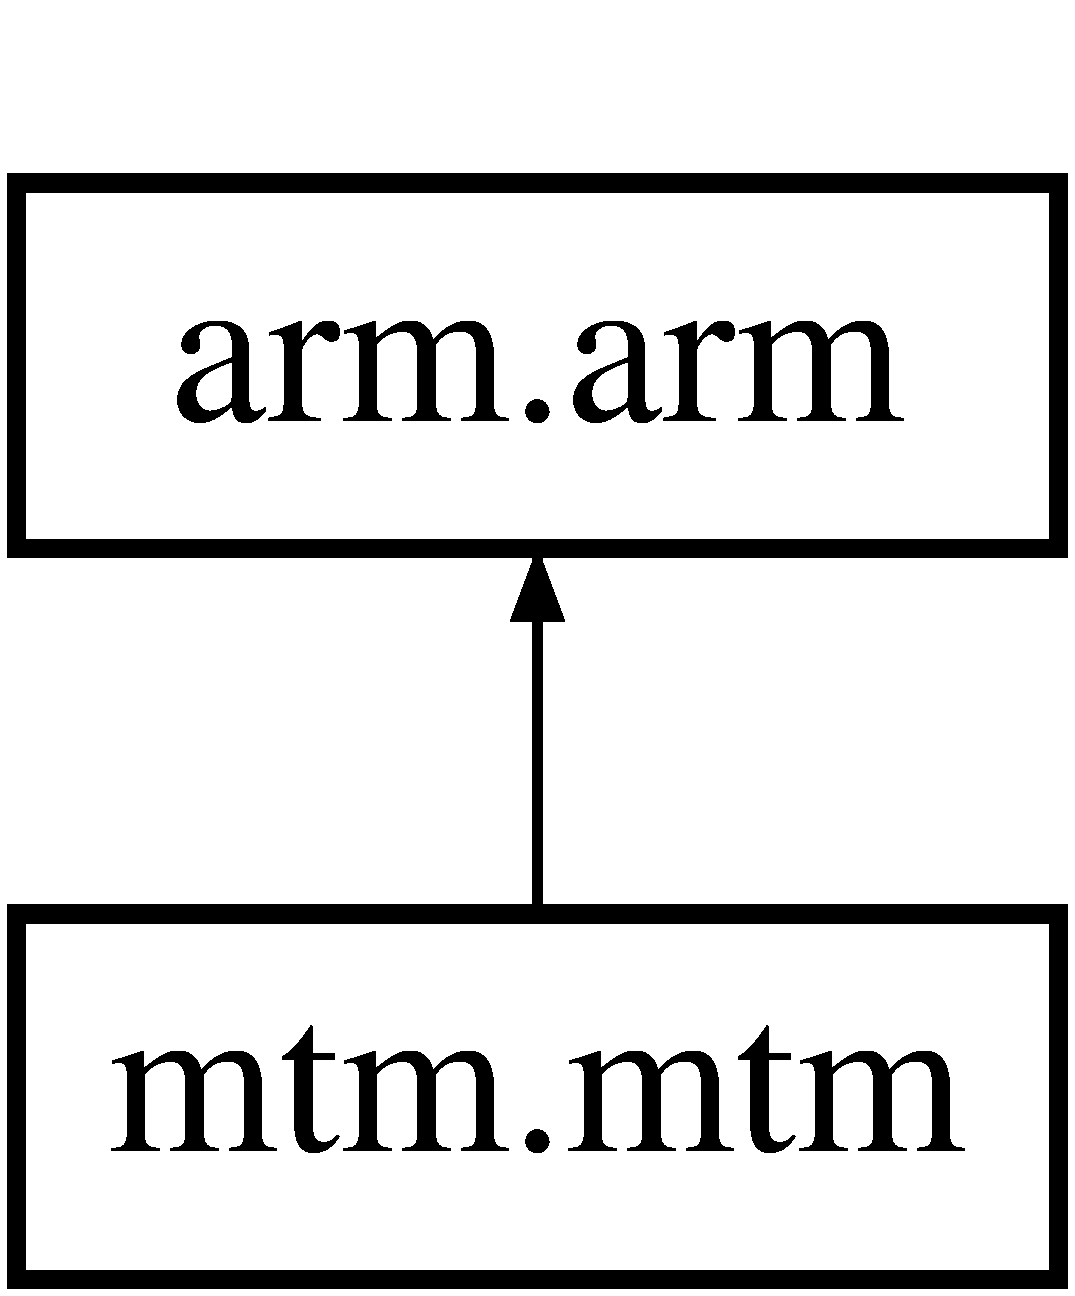
\includegraphics[height=2.000000cm]{classmtm_1_1mtm}
\end{center}
\end{figure}
\subsection*{Public Member Functions}
\begin{DoxyCompactItemize}
\item 
\hypertarget{classmtm_1_1mtm_a7bc909df85ca3bc9f6fc75eca32bafe6}{def {\bfseries \-\_\-\-\_\-init\-\_\-\-\_\-}}\label{classmtm_1_1mtm_a7bc909df85ca3bc9f6fc75eca32bafe6}

\item 
\hypertarget{classmtm_1_1mtm_a45de9466c32810b8670e724527c100a7}{def {\bfseries unregister}}\label{classmtm_1_1mtm_a45de9466c32810b8670e724527c100a7}

\item 
\hypertarget{classmtm_1_1mtm_a0e39b47e613b060621e483090edabeaa}{def {\bfseries lock\-\_\-orientation\-\_\-as\-\_\-is}}\label{classmtm_1_1mtm_a0e39b47e613b060621e483090edabeaa}

\item 
\hypertarget{classmtm_1_1mtm_a027de16f78002ef6d6b0e7d0af887ba1}{def {\bfseries lock\-\_\-orientation}}\label{classmtm_1_1mtm_a027de16f78002ef6d6b0e7d0af887ba1}

\item 
\hypertarget{classmtm_1_1mtm_ae69bc9cd377cf8c5a6af0ab451a0aa32}{def {\bfseries unlock\-\_\-orientation}}\label{classmtm_1_1mtm_ae69bc9cd377cf8c5a6af0ab451a0aa32}

\end{DoxyCompactItemize}
\subsection*{Public Attributes}
\begin{DoxyCompactItemize}
\item 
\hypertarget{classmtm_1_1mtm_a51dd418527ef857a52295ccf74a876b2}{{\bfseries lock\-\_\-orientation\-\_\-publisher}}\label{classmtm_1_1mtm_a51dd418527ef857a52295ccf74a876b2}

\item 
\hypertarget{classmtm_1_1mtm_a8fda57c86f322f0dec30eb5ab40fd714}{{\bfseries unlock\-\_\-orientation\-\_\-publisher}}\label{classmtm_1_1mtm_a8fda57c86f322f0dec30eb5ab40fd714}

\end{DoxyCompactItemize}


\subsection{Detailed Description}
\begin{DoxyVerb}Simple robot API wrapping around ROS messages
\end{DoxyVerb}
 

The documentation for this class was generated from the following file\-:\begin{DoxyCompactItemize}
\item 
mtm.\-py\end{DoxyCompactItemize}

\hypertarget{classmtm__alignment__test_1_1mtm__aligner}{\section{mtm\-\_\-alignment\-\_\-test.\-mtm\-\_\-aligner Class Reference}
\label{classmtm__alignment__test_1_1mtm__aligner}\index{mtm\-\_\-alignment\-\_\-test.\-mtm\-\_\-aligner@{mtm\-\_\-alignment\-\_\-test.\-mtm\-\_\-aligner}}
}
\subsection*{Public Member Functions}
\begin{DoxyCompactItemize}
\item 
def \hyperlink{classmtm__alignment__test_1_1mtm__aligner_ae8bb0d4f0b12e149f1032b18ee13754f}{rotate}
\item 
\hypertarget{classmtm__alignment__test_1_1mtm__aligner_a356851f1dbf80bfdf88dd2be2375aadf}{def {\bfseries ecm\-\_\-joint\-\_\-cb}}\label{classmtm__alignment__test_1_1mtm__aligner_a356851f1dbf80bfdf88dd2be2375aadf}

\item 
\hypertarget{classmtm__alignment__test_1_1mtm__aligner_a86b062fc65be35830ad5239d1c453aca}{def {\bfseries \-\_\-\-\_\-init\-\_\-\-\_\-}}\label{classmtm__alignment__test_1_1mtm__aligner_a86b062fc65be35830ad5239d1c453aca}

\end{DoxyCompactItemize}
\subsection*{Public Attributes}
\begin{DoxyCompactItemize}
\item 
\hypertarget{classmtm__alignment__test_1_1mtm__aligner_a66fbb0a8962ef5b3b28fe1429315d5cc}{{\bfseries lets\-\_\-do\-\_\-it\-\_\-once}}\label{classmtm__alignment__test_1_1mtm__aligner_a66fbb0a8962ef5b3b28fe1429315d5cc}

\item 
\hypertarget{classmtm__alignment__test_1_1mtm__aligner_aa0457188df6f6daf8af6fc7ba9ba4242}{{\bfseries psm1\-\_\-kin}}\label{classmtm__alignment__test_1_1mtm__aligner_aa0457188df6f6daf8af6fc7ba9ba4242}

\item 
\hypertarget{classmtm__alignment__test_1_1mtm__aligner_ab10272a41958344050deb06e813cd82d}{{\bfseries psm1\-\_\-robot}}\label{classmtm__alignment__test_1_1mtm__aligner_ab10272a41958344050deb06e813cd82d}

\item 
\hypertarget{classmtm__alignment__test_1_1mtm__aligner_a41fa48a02c1b1a94d13058083c6fe6f4}{{\bfseries psm2\-\_\-kin}}\label{classmtm__alignment__test_1_1mtm__aligner_a41fa48a02c1b1a94d13058083c6fe6f4}

\item 
\hypertarget{classmtm__alignment__test_1_1mtm__aligner_a9b788a92a4b18e8740f90d9fd16c34c2}{{\bfseries psm2\-\_\-robot}}\label{classmtm__alignment__test_1_1mtm__aligner_a9b788a92a4b18e8740f90d9fd16c34c2}

\item 
\hypertarget{classmtm__alignment__test_1_1mtm__aligner_ab719e5232dcd65bdccb822165b231450}{{\bfseries ecm\-\_\-kin}}\label{classmtm__alignment__test_1_1mtm__aligner_ab719e5232dcd65bdccb822165b231450}

\item 
\hypertarget{classmtm__alignment__test_1_1mtm__aligner_a2172ccdef3463694da08c63704888fdc}{{\bfseries ecm\-\_\-robot}}\label{classmtm__alignment__test_1_1mtm__aligner_a2172ccdef3463694da08c63704888fdc}

\item 
\hypertarget{classmtm__alignment__test_1_1mtm__aligner_ab4698ffb0769df9a323b4fdf2ea6dd14}{{\bfseries mtmr\-\_\-robot}}\label{classmtm__alignment__test_1_1mtm__aligner_ab4698ffb0769df9a323b4fdf2ea6dd14}

\item 
\hypertarget{classmtm__alignment__test_1_1mtm__aligner_a681ac32ad367833eb3114fa3ddf133c9}{{\bfseries mtmr\-\_\-kin}}\label{classmtm__alignment__test_1_1mtm__aligner_a681ac32ad367833eb3114fa3ddf133c9}

\item 
\hypertarget{classmtm__alignment__test_1_1mtm__aligner_a2722555b351f9cd18b6c4c3203228117}{{\bfseries psm1\-\_\-pub}}\label{classmtm__alignment__test_1_1mtm__aligner_a2722555b351f9cd18b6c4c3203228117}

\item 
\hypertarget{classmtm__alignment__test_1_1mtm__aligner_ad8672e13dfd606b4a77b68403adc6e73}{{\bfseries psm2\-\_\-pub}}\label{classmtm__alignment__test_1_1mtm__aligner_ad8672e13dfd606b4a77b68403adc6e73}

\item 
\hypertarget{classmtm__alignment__test_1_1mtm__aligner_a261a2258c62f232c6f789d71e4d30de6}{{\bfseries ecm\-\_\-pub}}\label{classmtm__alignment__test_1_1mtm__aligner_a261a2258c62f232c6f789d71e4d30de6}

\item 
\hypertarget{classmtm__alignment__test_1_1mtm__aligner_a6b0f4eddab2fdafe95d7d6c916db58ee}{{\bfseries mtmr\-\_\-pub}}\label{classmtm__alignment__test_1_1mtm__aligner_a6b0f4eddab2fdafe95d7d6c916db58ee}

\item 
\hypertarget{classmtm__alignment__test_1_1mtm__aligner_a6e296d6faef8bbbef41f7a4fefefe6fb}{{\bfseries mtml\-\_\-pub}}\label{classmtm__alignment__test_1_1mtm__aligner_a6e296d6faef8bbbef41f7a4fefefe6fb}

\item 
\hypertarget{classmtm__alignment__test_1_1mtm__aligner_a3838fa4b092feb3f441472e006df6a93}{{\bfseries ecm\-\_\-base}}\label{classmtm__alignment__test_1_1mtm__aligner_a3838fa4b092feb3f441472e006df6a93}

\item 
\hypertarget{classmtm__alignment__test_1_1mtm__aligner_a83df974e499509163d717369caf24ef4}{{\bfseries tf\-\_\-new\-\_\-psm2\-\_\-base}}\label{classmtm__alignment__test_1_1mtm__aligner_a83df974e499509163d717369caf24ef4}

\item 
\hypertarget{classmtm__alignment__test_1_1mtm__aligner_a6cc554ce6b26af83da6867df9784821a}{{\bfseries tf\-\_\-new\-\_\-psm1\-\_\-base}}\label{classmtm__alignment__test_1_1mtm__aligner_a6cc554ce6b26af83da6867df9784821a}

\item 
\hypertarget{classmtm__alignment__test_1_1mtm__aligner_acb3f9429ac21c843a006489a202070a5}{{\bfseries mtmr\-\_\-base}}\label{classmtm__alignment__test_1_1mtm__aligner_acb3f9429ac21c843a006489a202070a5}

\item 
\hypertarget{classmtm__alignment__test_1_1mtm__aligner_a3c7cbcff7ef9b58a3d390f5f12d5273b}{{\bfseries mtmr\-\_\-hw}}\label{classmtm__alignment__test_1_1mtm__aligner_a3c7cbcff7ef9b58a3d390f5f12d5273b}

\item 
\hypertarget{classmtm__alignment__test_1_1mtm__aligner_abff688327c863eef627434bf191a1ced}{{\bfseries mtml\-\_\-hw}}\label{classmtm__alignment__test_1_1mtm__aligner_abff688327c863eef627434bf191a1ced}

\item 
\hypertarget{classmtm__alignment__test_1_1mtm__aligner_a87073e1b7a7361ae32ad98c018269438}{{\bfseries psm1\-\_\-hw}}\label{classmtm__alignment__test_1_1mtm__aligner_a87073e1b7a7361ae32ad98c018269438}

\item 
\hypertarget{classmtm__alignment__test_1_1mtm__aligner_ad095e8db3bc09f4f6a96187a4fda2cf9}{{\bfseries psm2\-\_\-hw}}\label{classmtm__alignment__test_1_1mtm__aligner_ad095e8db3bc09f4f6a96187a4fda2cf9}

\end{DoxyCompactItemize}
\subsection*{Static Public Attributes}
\begin{DoxyCompactItemize}
\item 
\hypertarget{classmtm__alignment__test_1_1mtm__aligner_a84768367a1e9952cd2be1f8bf6d77eb5}{{\bfseries q} = msg.\-position}\label{classmtm__alignment__test_1_1mtm__aligner_a84768367a1e9952cd2be1f8bf6d77eb5}

\item 
\hypertarget{classmtm__alignment__test_1_1mtm__aligner_a69769e0c07a10bac224ef50a9fd4070a}{tuple {\bfseries ecm\-\_\-ee} = self.\-ecm\-\_\-kin.\-forward(q)}\label{classmtm__alignment__test_1_1mtm__aligner_a69769e0c07a10bac224ef50a9fd4070a}

\item 
\hypertarget{classmtm__alignment__test_1_1mtm__aligner_a7cb6f99d5700f109f560cd6fa0dbc79f}{tuple {\bfseries ecm\-\_\-base\-\_\-frame} = self.\-ecm\-\_\-base.\-forward(\mbox{[}$\,$\mbox{]})}\label{classmtm__alignment__test_1_1mtm__aligner_a7cb6f99d5700f109f560cd6fa0dbc79f}

\item 
\hypertarget{classmtm__alignment__test_1_1mtm__aligner_ab41240ac9e3960dca058d464b7460874}{tuple {\bfseries r\-\_\-180\-\_\-x} = self.\-rotate('x', pi)}\label{classmtm__alignment__test_1_1mtm__aligner_ab41240ac9e3960dca058d464b7460874}

\item 
\hypertarget{classmtm__alignment__test_1_1mtm__aligner_a1353322b5bb40f0a5d8ef8ae6c644e95}{tuple {\bfseries r\-\_\-90\-\_\-z} = self.\-rotate('z', -\/pi/2)}\label{classmtm__alignment__test_1_1mtm__aligner_a1353322b5bb40f0a5d8ef8ae6c644e95}

\item 
\hypertarget{classmtm__alignment__test_1_1mtm__aligner_af550be8d65ace8a3e291ca55c19cbe41}{tuple {\bfseries psm1\-\_\-base\-\_\-frame} = (ecm\-\_\-ee $\ast$$\ast$ -\/1)}\label{classmtm__alignment__test_1_1mtm__aligner_af550be8d65ace8a3e291ca55c19cbe41}

\item 
\hypertarget{classmtm__alignment__test_1_1mtm__aligner_ab2bda5b0fb885d59bbc8d85226038db2}{tuple {\bfseries psm1\-\_\-message} = pose\-\_\-converter.\-Pose\-Conv.\-to\-\_\-pose\-\_\-msg(psm1\-\_\-base\-\_\-frame)}\label{classmtm__alignment__test_1_1mtm__aligner_ab2bda5b0fb885d59bbc8d85226038db2}

\item 
\hypertarget{classmtm__alignment__test_1_1mtm__aligner_a5ab5797fdbfebd015d215d9dbcb2929e}{tuple {\bfseries psm1\-\_\-message\-\_\-stamped} = pose\-\_\-converter.\-Pose\-Conv.\-to\-\_\-pose\-\_\-stamped\-\_\-msg(psm1\-\_\-base\-\_\-frame)}\label{classmtm__alignment__test_1_1mtm__aligner_a5ab5797fdbfebd015d215d9dbcb2929e}

\item 
\hypertarget{classmtm__alignment__test_1_1mtm__aligner_a3575f94b228b6d8998bb4c19f8f4cde9}{tuple {\bfseries psm2\-\_\-base\-\_\-frame} = (ecm\-\_\-ee $\ast$$\ast$ -\/1)}\label{classmtm__alignment__test_1_1mtm__aligner_a3575f94b228b6d8998bb4c19f8f4cde9}

\item 
\hypertarget{classmtm__alignment__test_1_1mtm__aligner_a08c8a821a4f07982873341c23fe4a09d}{tuple {\bfseries psm2\-\_\-message} = pose\-\_\-converter.\-Pose\-Conv.\-to\-\_\-pose\-\_\-msg(psm2\-\_\-base\-\_\-frame)}\label{classmtm__alignment__test_1_1mtm__aligner_a08c8a821a4f07982873341c23fe4a09d}

\item 
\hypertarget{classmtm__alignment__test_1_1mtm__aligner_a8c0374e589d2db89fd59e01dbfaef02f}{tuple {\bfseries psm2\-\_\-message\-\_\-stamped} = pose\-\_\-converter.\-Pose\-Conv.\-to\-\_\-pose\-\_\-stamped\-\_\-msg(psm2\-\_\-base\-\_\-frame)}\label{classmtm__alignment__test_1_1mtm__aligner_a8c0374e589d2db89fd59e01dbfaef02f}

\item 
\hypertarget{classmtm__alignment__test_1_1mtm__aligner_affd419c85a6756e4646051d811ac38ba}{tuple {\bfseries ecm\-\_\-message} = pose\-\_\-converter.\-Pose\-Conv.\-to\-\_\-pose\-\_\-msg(ecm\-\_\-base\-\_\-frame)}\label{classmtm__alignment__test_1_1mtm__aligner_affd419c85a6756e4646051d811ac38ba}

\item 
\hypertarget{classmtm__alignment__test_1_1mtm__aligner_add6c43296672eb784ced99b9e224f58e}{tuple {\bfseries ecm\-\_\-ee\-\_\-message\-\_\-stamped} = pose\-\_\-converter.\-Pose\-Conv.\-to\-\_\-pose\-\_\-stamped\-\_\-msg(ecm\-\_\-ee)}\label{classmtm__alignment__test_1_1mtm__aligner_add6c43296672eb784ced99b9e224f58e}

\end{DoxyCompactItemize}


\subsection{Member Function Documentation}
\hypertarget{classmtm__alignment__test_1_1mtm__aligner_ae8bb0d4f0b12e149f1032b18ee13754f}{\index{mtm\-\_\-alignment\-\_\-test\-::mtm\-\_\-aligner@{mtm\-\_\-alignment\-\_\-test\-::mtm\-\_\-aligner}!rotate@{rotate}}
\index{rotate@{rotate}!mtm_alignment_test::mtm_aligner@{mtm\-\_\-alignment\-\_\-test\-::mtm\-\_\-aligner}}
\subsubsection[{rotate}]{\setlength{\rightskip}{0pt plus 5cm}def mtm\-\_\-alignment\-\_\-test.\-mtm\-\_\-aligner.\-rotate (
\begin{DoxyParamCaption}
\item[{}]{self, }
\item[{}]{axis, }
\item[{}]{angle}
\end{DoxyParamCaption}
)}}\label{classmtm__alignment__test_1_1mtm__aligner_ae8bb0d4f0b12e149f1032b18ee13754f}
\begin{DoxyVerb}Returns a rotation matrix
    axis : 'x','y' or 'z'
    angle : In radians
\end{DoxyVerb}
 

The documentation for this class was generated from the following file\-:\begin{DoxyCompactItemize}
\item 
mtm\-\_\-alignment\-\_\-test.\-py\end{DoxyCompactItemize}

\hypertarget{classcamera__control__node_1_1camera__qt__gui_1_1node__name}{\section{camera\-\_\-control\-\_\-node.\-camera\-\_\-qt\-\_\-gui.\-node\-\_\-name Class Reference}
\label{classcamera__control__node_1_1camera__qt__gui_1_1node__name}\index{camera\-\_\-control\-\_\-node.\-camera\-\_\-qt\-\_\-gui.\-node\-\_\-name@{camera\-\_\-control\-\_\-node.\-camera\-\_\-qt\-\_\-gui.\-node\-\_\-name}}
}
\subsection*{Static Public Attributes}
\begin{DoxyCompactItemize}
\item 
\hypertarget{classcamera__control__node_1_1camera__qt__gui_1_1node__name_ab2a3486e7ae1f280e9006c66a138c9fe}{string {\bfseries clutch\-N\-Go} = 'clutch\-\_\-control'}\label{classcamera__control__node_1_1camera__qt__gui_1_1node__name_ab2a3486e7ae1f280e9006c66a138c9fe}

\item 
\hypertarget{classcamera__control__node_1_1camera__qt__gui_1_1node__name_ae1490012082c209d4ec7b46217377548}{string {\bfseries autocamera} = '\hyperlink{classautocamera__algorithm_1_1Autocamera}{Autocamera}'}\label{classcamera__control__node_1_1camera__qt__gui_1_1node__name_ae1490012082c209d4ec7b46217377548}

\item 
\hypertarget{classcamera__control__node_1_1camera__qt__gui_1_1node__name_acf51bf9c4f26c3ad9b4e7245ee98c908}{string {\bfseries joystick} = 'joystick'}\label{classcamera__control__node_1_1camera__qt__gui_1_1node__name_acf51bf9c4f26c3ad9b4e7245ee98c908}

\item 
\hypertarget{classcamera__control__node_1_1camera__qt__gui_1_1node__name_ad25806ce0f8bea28dd7cf9fedcd88736}{string {\bfseries teleop} = 'teleop'}\label{classcamera__control__node_1_1camera__qt__gui_1_1node__name_ad25806ce0f8bea28dd7cf9fedcd88736}

\item 
\hypertarget{classcamera__control__node_1_1camera__qt__gui_1_1node__name_a56c4826e721af6a03d3245287de73e1d}{string {\bfseries oculus} = 'oculus'}\label{classcamera__control__node_1_1camera__qt__gui_1_1node__name_a56c4826e721af6a03d3245287de73e1d}

\end{DoxyCompactItemize}


The documentation for this class was generated from the following file\-:\begin{DoxyCompactItemize}
\item 
camera\-\_\-control\-\_\-node.\-py\end{DoxyCompactItemize}

\hypertarget{classcamera__control__node_1_1Oculus}{\section{camera\-\_\-control\-\_\-node.\-Oculus Class Reference}
\label{classcamera__control__node_1_1Oculus}\index{camera\-\_\-control\-\_\-node.\-Oculus@{camera\-\_\-control\-\_\-node.\-Oculus}}
}
\subsection*{Classes}
\begin{DoxyCompactItemize}
\item 
class \hyperlink{classcamera__control__node_1_1Oculus_1_1MODE}{M\-O\-D\-E}
\end{DoxyCompactItemize}
\subsection*{Public Member Functions}
\begin{DoxyCompactItemize}
\item 
\hypertarget{classcamera__control__node_1_1Oculus_a554cfd3e83d216fc326c432fc5275ee0}{def {\bfseries \-\_\-\-\_\-init\-\_\-\-\_\-}}\label{classcamera__control__node_1_1Oculus_a554cfd3e83d216fc326c432fc5275ee0}

\item 
\hypertarget{classcamera__control__node_1_1Oculus_a3ac769306641ab398a75396bc408ad00}{def {\bfseries \-\_\-\-\_\-init\-\_\-nodes\-\_\-\-\_\-}}\label{classcamera__control__node_1_1Oculus_a3ac769306641ab398a75396bc408ad00}

\item 
\hypertarget{classcamera__control__node_1_1Oculus_af548f9f6cd4afc2a9ac9e7e0df2b4e32}{def {\bfseries shutdown}}\label{classcamera__control__node_1_1Oculus_af548f9f6cd4afc2a9ac9e7e0df2b4e32}

\item 
\hypertarget{classcamera__control__node_1_1Oculus_afbc337c97f67f8c70d1ef647a7526a1f}{def {\bfseries set\-\_\-mode}}\label{classcamera__control__node_1_1Oculus_afbc337c97f67f8c70d1ef647a7526a1f}

\item 
\hypertarget{classcamera__control__node_1_1Oculus_acb12601fd6198f50b3f24bc6dd69edf6}{def {\bfseries spin}}\label{classcamera__control__node_1_1Oculus_acb12601fd6198f50b3f24bc6dd69edf6}

\item 
\hypertarget{classcamera__control__node_1_1Oculus_a1c8efccd964a54297355e7cbbd6ec6d0}{def {\bfseries \-\_\-\-\_\-spin\-\_\-\-\_\-}}\label{classcamera__control__node_1_1Oculus_a1c8efccd964a54297355e7cbbd6ec6d0}

\item 
\hypertarget{classcamera__control__node_1_1Oculus_a257f09cbcb4b6808d8c0f595aa66af51}{def {\bfseries on\-\_\-oculus\-\_\-cb}}\label{classcamera__control__node_1_1Oculus_a257f09cbcb4b6808d8c0f595aa66af51}

\item 
\hypertarget{classcamera__control__node_1_1Oculus_a1211fb3f1116b04ee8f4f5f0a246bcea}{def {\bfseries \-\_\-\-\_\-ecm\-\_\-cb\-\_\-\-\_\-}}\label{classcamera__control__node_1_1Oculus_a1211fb3f1116b04ee8f4f5f0a246bcea}

\end{DoxyCompactItemize}
\subsection*{Public Attributes}
\begin{DoxyCompactItemize}
\item 
\hypertarget{classcamera__control__node_1_1Oculus_a674d456ebe0c26ad445e69c3c723d7cd}{{\bfseries joint\-\_\-angles}}\label{classcamera__control__node_1_1Oculus_a674d456ebe0c26ad445e69c3c723d7cd}

\item 
\hypertarget{classcamera__control__node_1_1Oculus_a0396d5a5a959b98a1f861b3ca964b5c5}{{\bfseries center}}\label{classcamera__control__node_1_1Oculus_a0396d5a5a959b98a1f861b3ca964b5c5}

\item 
\hypertarget{classcamera__control__node_1_1Oculus_ae11938b01123c1acf99d9c060f0a7473}{{\bfseries joystick\-\_\-at\-\_\-zero}}\label{classcamera__control__node_1_1Oculus_ae11938b01123c1acf99d9c060f0a7473}

\item 
\hypertarget{classcamera__control__node_1_1Oculus_a963a6efe4d9f8cec5791d82982f24ae4}{{\bfseries movement\-\_\-scale}}\label{classcamera__control__node_1_1Oculus_a963a6efe4d9f8cec5791d82982f24ae4}

\item 
\hypertarget{classcamera__control__node_1_1Oculus_a63ab92999bada1b51d0cdc67afd88909}{{\bfseries last\-\_\-z}}\label{classcamera__control__node_1_1Oculus_a63ab92999bada1b51d0cdc67afd88909}

\item 
\hypertarget{classcamera__control__node_1_1Oculus_aacfe5ec1cad6156dc390c95ac9fbf81f}{{\bfseries hw\-\_\-ecm}}\label{classcamera__control__node_1_1Oculus_aacfe5ec1cad6156dc390c95ac9fbf81f}

\item 
\hypertarget{classcamera__control__node_1_1Oculus_a34a40cdc4926c4fca15158d4c897fe83}{{\bfseries pub\-\_\-ecm\-\_\-sim}}\label{classcamera__control__node_1_1Oculus_a34a40cdc4926c4fca15158d4c897fe83}

\item 
\hypertarget{classcamera__control__node_1_1Oculus_ac7ac9c36491facca6f646c8e5494ec7e}{{\bfseries sub\-\_\-oculus}}\label{classcamera__control__node_1_1Oculus_ac7ac9c36491facca6f646c8e5494ec7e}

\end{DoxyCompactItemize}


The documentation for this class was generated from the following file\-:\begin{DoxyCompactItemize}
\item 
camera\-\_\-control\-\_\-node.\-py\end{DoxyCompactItemize}

\hypertarget{classpsm_1_1psm}{\section{psm.\-psm Class Reference}
\label{classpsm_1_1psm}\index{psm.\-psm@{psm.\-psm}}
}
Inheritance diagram for psm.\-psm\-:\begin{figure}[H]
\begin{center}
\leavevmode
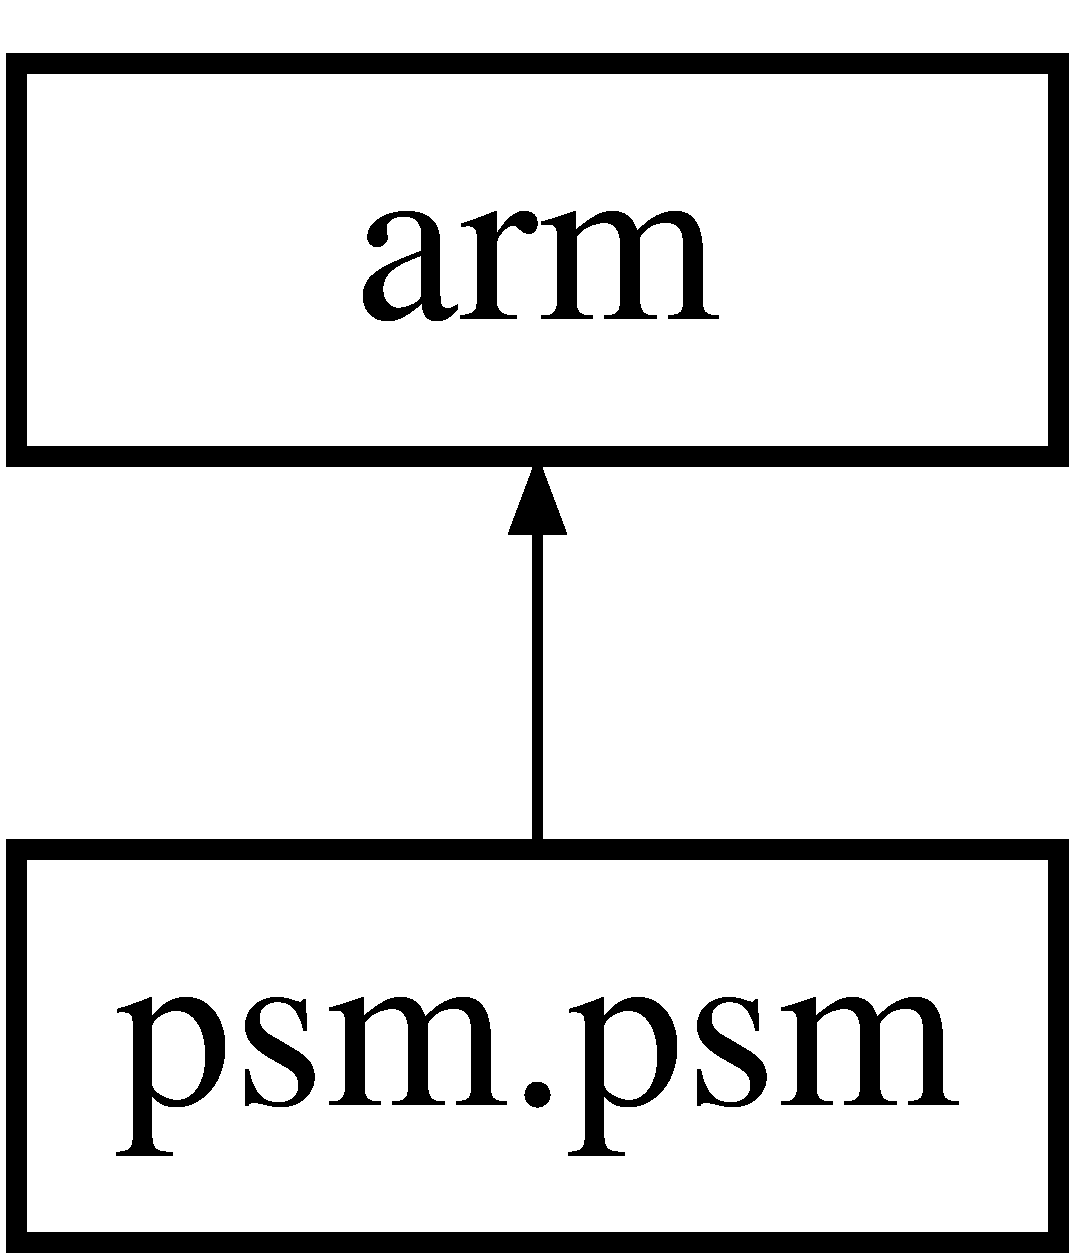
\includegraphics[height=2.000000cm]{classpsm_1_1psm}
\end{center}
\end{figure}
\subsection*{Public Member Functions}
\begin{DoxyCompactItemize}
\item 
\hypertarget{classpsm_1_1psm_a86afec832f80d1f08e6a6994c2942522}{def {\bfseries \-\_\-\-\_\-init\-\_\-\-\_\-}}\label{classpsm_1_1psm_a86afec832f80d1f08e6a6994c2942522}

\item 
\hypertarget{classpsm_1_1psm_a3fcfa4ee214b49701bcc24d167d4c8bc}{def {\bfseries close\-\_\-jaw}}\label{classpsm_1_1psm_a3fcfa4ee214b49701bcc24d167d4c8bc}

\item 
\hypertarget{classpsm_1_1psm_a5cca1190afe164269f5481b330e77e13}{def {\bfseries open\-\_\-jaw}}\label{classpsm_1_1psm_a5cca1190afe164269f5481b330e77e13}

\item 
\hypertarget{classpsm_1_1psm_a66a9d98a15f34996eaa88ffd32a1bac0}{def {\bfseries set\-\_\-jaw}}\label{classpsm_1_1psm_a66a9d98a15f34996eaa88ffd32a1bac0}

\end{DoxyCompactItemize}
\subsection*{Public Attributes}
\begin{DoxyCompactItemize}
\item 
\hypertarget{classpsm_1_1psm_a21845195746b53c80d7b49e011bde0c4}{{\bfseries set\-\_\-jaw\-\_\-position\-\_\-publisher}}\label{classpsm_1_1psm_a21845195746b53c80d7b49e011bde0c4}

\end{DoxyCompactItemize}


\subsection{Detailed Description}
\begin{DoxyVerb}Simple robot API wrapping around ROS messages
\end{DoxyVerb}
 

The documentation for this class was generated from the following file\-:\begin{DoxyCompactItemize}
\item 
psm.\-py\end{DoxyCompactItemize}

\hypertarget{classbase__coregistration_1_1coregistrator_1_1REGISTRATION__MODE}{\section{base\-\_\-coregistration.\-coregistrator.\-R\-E\-G\-I\-S\-T\-R\-A\-T\-I\-O\-N\-\_\-\-M\-O\-D\-E Class Reference}
\label{classbase__coregistration_1_1coregistrator_1_1REGISTRATION__MODE}\index{base\-\_\-coregistration.\-coregistrator.\-R\-E\-G\-I\-S\-T\-R\-A\-T\-I\-O\-N\-\_\-\-M\-O\-D\-E@{base\-\_\-coregistration.\-coregistrator.\-R\-E\-G\-I\-S\-T\-R\-A\-T\-I\-O\-N\-\_\-\-M\-O\-D\-E}}
}
\subsection*{Static Public Attributes}
\begin{DoxyCompactItemize}
\item 
\hypertarget{classbase__coregistration_1_1coregistrator_1_1REGISTRATION__MODE_a98539fedf84ca1f98c64168cd6137edc}{string {\bfseries P\-S\-M1\-\_\-\-P\-S\-M2} = 'psm1\-\_\-psm2'}\label{classbase__coregistration_1_1coregistrator_1_1REGISTRATION__MODE_a98539fedf84ca1f98c64168cd6137edc}

\item 
\hypertarget{classbase__coregistration_1_1coregistrator_1_1REGISTRATION__MODE_a799ae877f68cca5f7615751c9e5aafc2}{string {\bfseries P\-S\-M1\-\_\-\-E\-C\-M} = 'psm1\-\_\-ecm'}\label{classbase__coregistration_1_1coregistrator_1_1REGISTRATION__MODE_a799ae877f68cca5f7615751c9e5aafc2}

\end{DoxyCompactItemize}


\subsection{Detailed Description}
\begin{DoxyVerb}    The registration mode. 
\end{DoxyVerb}
 

The documentation for this class was generated from the following file\-:\begin{DoxyCompactItemize}
\item 
base\-\_\-coregistration.\-py\end{DoxyCompactItemize}

\hypertarget{classrobot_1_1robot}{\section{robot.\-robot Class Reference}
\label{classrobot_1_1robot}\index{robot.\-robot@{robot.\-robot}}
}
\subsection*{Public Member Functions}
\begin{DoxyCompactItemize}
\item 
def \hyperlink{classrobot_1_1robot_ada0f0d621d7b7f3c82f103ca39655e57}{\-\_\-\-\_\-init\-\_\-\-\_\-}
\item 
def \hyperlink{classrobot_1_1robot_acfcfba4c2e3a5fff6a16bbfa23a43f0b}{home}
\item 
def \hyperlink{classrobot_1_1robot_a269263585bfeaf41c99cb917fbd3b2a4}{shutdown}
\item 
\hypertarget{classrobot_1_1robot_a269754c183476c1af79982fad7a913aa}{def {\bfseries get\-\_\-robot\-\_\-state}}\label{classrobot_1_1robot_a269754c183476c1af79982fad7a913aa}

\item 
def \hyperlink{classrobot_1_1robot_a24d47d697c485ec681cea22d1b5d2eef}{get\-\_\-current\-\_\-cartesian\-\_\-position}
\item 
def \hyperlink{classrobot_1_1robot_a65a10aad3fb07d7b740c5aeb6a98f4fe}{get\-\_\-current\-\_\-joint\-\_\-position}
\item 
def \hyperlink{classrobot_1_1robot_a3f936417edb192eea87094cf4f1ebf81}{get\-\_\-current\-\_\-joint\-\_\-velocity}
\item 
def \hyperlink{classrobot_1_1robot_a69ee320aa8bd577693a86dc57edbe88d}{get\-\_\-current\-\_\-joint\-\_\-effort}
\item 
def \hyperlink{classrobot_1_1robot_a6c1363d7ee90df1bd551d21c4bf85405}{get\-\_\-desired\-\_\-cartesian\-\_\-position}
\item 
def \hyperlink{classrobot_1_1robot_a8ad506ad78ebcbf8537d68acd3221d46}{get\-\_\-desired\-\_\-joint\-\_\-position}
\item 
def \hyperlink{classrobot_1_1robot_acb3f4d16c51d3285750c6b102f435ecd}{get\-\_\-desired\-\_\-joint\-\_\-effort}
\item 
def \hyperlink{classrobot_1_1robot_a3381917875e5eb4a2580f89d30a29048}{get\-\_\-joint\-\_\-number}
\item 
\hypertarget{classrobot_1_1robot_ad9aa35ed46f7d41e0942474de6a048bd}{def {\bfseries close\-\_\-gripper}}\label{classrobot_1_1robot_ad9aa35ed46f7d41e0942474de6a048bd}

\item 
\hypertarget{classrobot_1_1robot_a729f68a055e67156c3ce045cc2fd0fc2}{def {\bfseries open\-\_\-gripper}}\label{classrobot_1_1robot_a729f68a055e67156c3ce045cc2fd0fc2}

\item 
def \hyperlink{classrobot_1_1robot_a0a0558344e70e559ab0b495f8a8843ea}{delta\-\_\-move\-\_\-cartesian}
\item 
def \hyperlink{classrobot_1_1robot_a450c1237abfeac7e579a166c6c962011}{delta\-\_\-move\-\_\-cartesian\-\_\-translation}
\item 
def \hyperlink{classrobot_1_1robot_a6c58255581206c373ae32f5d36018259}{delta\-\_\-move\-\_\-cartesian\-\_\-rotation}
\item 
def \hyperlink{classrobot_1_1robot_a4798dee826a80b1d49ff6c76702eb701}{delta\-\_\-move\-\_\-cartesian\-\_\-frame}
\item 
def \hyperlink{classrobot_1_1robot_ab19b349b7b70b282e4ef9ace5a9189ab}{move\-\_\-cartesian\-\_\-translation}
\item 
def \hyperlink{classrobot_1_1robot_aba6e20a98509ff70723bd1a7bcfd946a}{move\-\_\-cartesian}
\item 
def \hyperlink{classrobot_1_1robot_a6e05c44c0b6bea15a811752544e1e5d8}{move\-\_\-cartesian\-\_\-rotation}
\item 
def \hyperlink{classrobot_1_1robot_ab38bde7945284b6108288792864f8f32}{move\-\_\-cartesian\-\_\-frame}
\item 
def \hyperlink{classrobot_1_1robot_a5bf5efcbec5d06469378276ca5e2a793}{delta\-\_\-move\-\_\-joint\-\_\-list}
\item 
def \hyperlink{classrobot_1_1robot_a812b749bc6ca437a45ffd8ec2eca7e73}{move\-\_\-joint\-\_\-list}
\end{DoxyCompactItemize}
\subsection*{Public Attributes}
\begin{DoxyCompactItemize}
\item 
\hypertarget{classrobot_1_1robot_ad698c604b6b8318976849b9a44e4f775}{{\bfseries set\-\_\-robot\-\_\-state}}\label{classrobot_1_1robot_ad698c604b6b8318976849b9a44e4f775}

\item 
\hypertarget{classrobot_1_1robot_a604b77e634cb6390e1de61ce74ccbd94}{{\bfseries set\-\_\-position\-\_\-joint}}\label{classrobot_1_1robot_a604b77e634cb6390e1de61ce74ccbd94}

\item 
\hypertarget{classrobot_1_1robot_aa07a50d20eb6ae8f87f16ba2e5b5ec9f}{{\bfseries set\-\_\-position\-\_\-goal\-\_\-joint}}\label{classrobot_1_1robot_aa07a50d20eb6ae8f87f16ba2e5b5ec9f}

\item 
\hypertarget{classrobot_1_1robot_a1b4faee5ddf60a680f6db7dd60de34aa}{{\bfseries set\-\_\-position\-\_\-cartesian}}\label{classrobot_1_1robot_a1b4faee5ddf60a680f6db7dd60de34aa}

\item 
\hypertarget{classrobot_1_1robot_a904fcdae041ae610dd619ca4ce9d1c5a}{{\bfseries set\-\_\-position\-\_\-goal\-\_\-cartesian}}\label{classrobot_1_1robot_a904fcdae041ae610dd619ca4ce9d1c5a}

\item 
\hypertarget{classrobot_1_1robot_ae7c8300b89e37f05be231dc4201a3312}{{\bfseries set\-\_\-jaw\-\_\-position}}\label{classrobot_1_1robot_ae7c8300b89e37f05be231dc4201a3312}

\end{DoxyCompactItemize}


\subsection{Detailed Description}
\begin{DoxyVerb}Simple robot API wrapping around ROS messages
\end{DoxyVerb}
 

\subsection{Constructor \& Destructor Documentation}
\hypertarget{classrobot_1_1robot_ada0f0d621d7b7f3c82f103ca39655e57}{\index{robot\-::robot@{robot\-::robot}!\-\_\-\-\_\-init\-\_\-\-\_\-@{\-\_\-\-\_\-init\-\_\-\-\_\-}}
\index{\-\_\-\-\_\-init\-\_\-\-\_\-@{\-\_\-\-\_\-init\-\_\-\-\_\-}!robot::robot@{robot\-::robot}}
\subsubsection[{\-\_\-\-\_\-init\-\_\-\-\_\-}]{\setlength{\rightskip}{0pt plus 5cm}def robot.\-robot.\-\_\-\-\_\-init\-\_\-\-\_\- (
\begin{DoxyParamCaption}
\item[{}]{self, }
\item[{}]{robot\-\_\-name, }
\item[{}]{ros\-\_\-namespace = {\ttfamily '/dvrk/'}}
\end{DoxyParamCaption}
)}}\label{classrobot_1_1robot_ada0f0d621d7b7f3c82f103ca39655e57}
\begin{DoxyVerb}Constructor.  This initializes a few data members.It
requires a robot name, this will be used to find the ROS
topics for the robot being controlled.  For example if the
user wants `PSM1`, the ROS topics will be from the namespace
`/dvrk/PSM1`\end{DoxyVerb}
 

\subsection{Member Function Documentation}
\hypertarget{classrobot_1_1robot_a0a0558344e70e559ab0b495f8a8843ea}{\index{robot\-::robot@{robot\-::robot}!delta\-\_\-move\-\_\-cartesian@{delta\-\_\-move\-\_\-cartesian}}
\index{delta\-\_\-move\-\_\-cartesian@{delta\-\_\-move\-\_\-cartesian}!robot::robot@{robot\-::robot}}
\subsubsection[{delta\-\_\-move\-\_\-cartesian}]{\setlength{\rightskip}{0pt plus 5cm}def robot.\-robot.\-delta\-\_\-move\-\_\-cartesian (
\begin{DoxyParamCaption}
\item[{}]{self, }
\item[{}]{delta\-\_\-input, }
\item[{}]{interpolate = {\ttfamily True}}
\end{DoxyParamCaption}
)}}\label{classrobot_1_1robot_a0a0558344e70e559ab0b495f8a8843ea}
\begin{DoxyVerb}Incremental translation in cartesian space.

:param delta_input: the incremental translation you want to make
:param interpolate: see  :ref:`interpolate <interpolate>`
\end{DoxyVerb}
 \hypertarget{classrobot_1_1robot_a4798dee826a80b1d49ff6c76702eb701}{\index{robot\-::robot@{robot\-::robot}!delta\-\_\-move\-\_\-cartesian\-\_\-frame@{delta\-\_\-move\-\_\-cartesian\-\_\-frame}}
\index{delta\-\_\-move\-\_\-cartesian\-\_\-frame@{delta\-\_\-move\-\_\-cartesian\-\_\-frame}!robot::robot@{robot\-::robot}}
\subsubsection[{delta\-\_\-move\-\_\-cartesian\-\_\-frame}]{\setlength{\rightskip}{0pt plus 5cm}def robot.\-robot.\-delta\-\_\-move\-\_\-cartesian\-\_\-frame (
\begin{DoxyParamCaption}
\item[{}]{self, }
\item[{}]{delta\-\_\-frame, }
\item[{}]{interpolate = {\ttfamily True}}
\end{DoxyParamCaption}
)}}\label{classrobot_1_1robot_a4798dee826a80b1d49ff6c76702eb701}
\begin{DoxyVerb}Incremental move by Frame in cartesian plane.

:param delta_frame: the incremental `PyKDL.Frame <http://docs.ros.org/diamondback/api/kdl/html/python/geometric_primitives.html>`_ based upon the current position
:param interpolate: see  :ref:`interpolate <interpolate>`\end{DoxyVerb}
 \hypertarget{classrobot_1_1robot_a6c58255581206c373ae32f5d36018259}{\index{robot\-::robot@{robot\-::robot}!delta\-\_\-move\-\_\-cartesian\-\_\-rotation@{delta\-\_\-move\-\_\-cartesian\-\_\-rotation}}
\index{delta\-\_\-move\-\_\-cartesian\-\_\-rotation@{delta\-\_\-move\-\_\-cartesian\-\_\-rotation}!robot::robot@{robot\-::robot}}
\subsubsection[{delta\-\_\-move\-\_\-cartesian\-\_\-rotation}]{\setlength{\rightskip}{0pt plus 5cm}def robot.\-robot.\-delta\-\_\-move\-\_\-cartesian\-\_\-rotation (
\begin{DoxyParamCaption}
\item[{}]{self, }
\item[{}]{delta\-\_\-rotation, }
\item[{}]{interpolate = {\ttfamily True}}
\end{DoxyParamCaption}
)}}\label{classrobot_1_1robot_a6c58255581206c373ae32f5d36018259}
\begin{DoxyVerb}Incremental rotation in cartesian plane.

:param delta_rotation: the incremental `PyKDL.Rotation <http://docs.ros.org/diamondback/api/kdl/html/python/geometric_primitives.html>`_ based upon the current position
:param interpolate: see  :ref:`interpolate <interpolate>`\end{DoxyVerb}
 \hypertarget{classrobot_1_1robot_a450c1237abfeac7e579a166c6c962011}{\index{robot\-::robot@{robot\-::robot}!delta\-\_\-move\-\_\-cartesian\-\_\-translation@{delta\-\_\-move\-\_\-cartesian\-\_\-translation}}
\index{delta\-\_\-move\-\_\-cartesian\-\_\-translation@{delta\-\_\-move\-\_\-cartesian\-\_\-translation}!robot::robot@{robot\-::robot}}
\subsubsection[{delta\-\_\-move\-\_\-cartesian\-\_\-translation}]{\setlength{\rightskip}{0pt plus 5cm}def robot.\-robot.\-delta\-\_\-move\-\_\-cartesian\-\_\-translation (
\begin{DoxyParamCaption}
\item[{}]{self, }
\item[{}]{delta\-\_\-translation, }
\item[{}]{interpolate = {\ttfamily True}}
\end{DoxyParamCaption}
)}}\label{classrobot_1_1robot_a450c1237abfeac7e579a166c6c962011}
\begin{DoxyVerb}Incremental translation in cartesian space.

:param delta_translation: the incremental translation you want to make based on the current position, this is in terms of a  `PyKDL.Vector <http://docs.ros.org/diamondback/api/kdl/html/python/geometric_primitives.html>`_ or a list of floats of size 3
:param interpolate: see  :ref:`interpolate <interpolate>`\end{DoxyVerb}
 \hypertarget{classrobot_1_1robot_a5bf5efcbec5d06469378276ca5e2a793}{\index{robot\-::robot@{robot\-::robot}!delta\-\_\-move\-\_\-joint\-\_\-list@{delta\-\_\-move\-\_\-joint\-\_\-list}}
\index{delta\-\_\-move\-\_\-joint\-\_\-list@{delta\-\_\-move\-\_\-joint\-\_\-list}!robot::robot@{robot\-::robot}}
\subsubsection[{delta\-\_\-move\-\_\-joint\-\_\-list}]{\setlength{\rightskip}{0pt plus 5cm}def robot.\-robot.\-delta\-\_\-move\-\_\-joint\-\_\-list (
\begin{DoxyParamCaption}
\item[{}]{self, }
\item[{}]{value, }
\item[{}]{index = {\ttfamily \mbox{[}\mbox{]}}, }
\item[{}]{interpolate = {\ttfamily True}}
\end{DoxyParamCaption}
)}}\label{classrobot_1_1robot_a5bf5efcbec5d06469378276ca5e2a793}
\begin{DoxyVerb}Incremental index move in joint space.

:param value: the incremental amount in which you want to move index by, this is a list
:param index: the joint you want to move, this is a list
:param interpolate: see  :ref:`interpolate <interpolate>`\end{DoxyVerb}
 \hypertarget{classrobot_1_1robot_a24d47d697c485ec681cea22d1b5d2eef}{\index{robot\-::robot@{robot\-::robot}!get\-\_\-current\-\_\-cartesian\-\_\-position@{get\-\_\-current\-\_\-cartesian\-\_\-position}}
\index{get\-\_\-current\-\_\-cartesian\-\_\-position@{get\-\_\-current\-\_\-cartesian\-\_\-position}!robot::robot@{robot\-::robot}}
\subsubsection[{get\-\_\-current\-\_\-cartesian\-\_\-position}]{\setlength{\rightskip}{0pt plus 5cm}def robot.\-robot.\-get\-\_\-current\-\_\-cartesian\-\_\-position (
\begin{DoxyParamCaption}
\item[{}]{self}
\end{DoxyParamCaption}
)}}\label{classrobot_1_1robot_a24d47d697c485ec681cea22d1b5d2eef}
\begin{DoxyVerb}Gets the :ref:`current cartesian position <currentvdesired>` of the robot in terms of cartesian space.

:returns: the current position of the robot in cartesian space
:rtype: `PyKDL.Frame <http://docs.ros.org/diamondback/api/kdl/html/python/geometric_primitives.html>`_\end{DoxyVerb}
 \hypertarget{classrobot_1_1robot_a69ee320aa8bd577693a86dc57edbe88d}{\index{robot\-::robot@{robot\-::robot}!get\-\_\-current\-\_\-joint\-\_\-effort@{get\-\_\-current\-\_\-joint\-\_\-effort}}
\index{get\-\_\-current\-\_\-joint\-\_\-effort@{get\-\_\-current\-\_\-joint\-\_\-effort}!robot::robot@{robot\-::robot}}
\subsubsection[{get\-\_\-current\-\_\-joint\-\_\-effort}]{\setlength{\rightskip}{0pt plus 5cm}def robot.\-robot.\-get\-\_\-current\-\_\-joint\-\_\-effort (
\begin{DoxyParamCaption}
\item[{}]{self}
\end{DoxyParamCaption}
)}}\label{classrobot_1_1robot_a69ee320aa8bd577693a86dc57edbe88d}
\begin{DoxyVerb}Gets the :ref:`current joint effort <currentvdesired>` of the robot in terms of joint space.

:returns: the current position of the robot in joint space
:rtype: `JointState <http://docs.ros.org/api/sensor_msgs/html/msg/JointState.html>`_\end{DoxyVerb}
 \hypertarget{classrobot_1_1robot_a65a10aad3fb07d7b740c5aeb6a98f4fe}{\index{robot\-::robot@{robot\-::robot}!get\-\_\-current\-\_\-joint\-\_\-position@{get\-\_\-current\-\_\-joint\-\_\-position}}
\index{get\-\_\-current\-\_\-joint\-\_\-position@{get\-\_\-current\-\_\-joint\-\_\-position}!robot::robot@{robot\-::robot}}
\subsubsection[{get\-\_\-current\-\_\-joint\-\_\-position}]{\setlength{\rightskip}{0pt plus 5cm}def robot.\-robot.\-get\-\_\-current\-\_\-joint\-\_\-position (
\begin{DoxyParamCaption}
\item[{}]{self}
\end{DoxyParamCaption}
)}}\label{classrobot_1_1robot_a65a10aad3fb07d7b740c5aeb6a98f4fe}
\begin{DoxyVerb}Gets the :ref:`current joint position <currentvdesired>` of the robot in terms of joint space.

:returns: the current position of the robot in joint space
:rtype: `JointState <http://docs.ros.org/api/sensor_msgs/html/msg/JointState.html>`_\end{DoxyVerb}
 \hypertarget{classrobot_1_1robot_a3f936417edb192eea87094cf4f1ebf81}{\index{robot\-::robot@{robot\-::robot}!get\-\_\-current\-\_\-joint\-\_\-velocity@{get\-\_\-current\-\_\-joint\-\_\-velocity}}
\index{get\-\_\-current\-\_\-joint\-\_\-velocity@{get\-\_\-current\-\_\-joint\-\_\-velocity}!robot::robot@{robot\-::robot}}
\subsubsection[{get\-\_\-current\-\_\-joint\-\_\-velocity}]{\setlength{\rightskip}{0pt plus 5cm}def robot.\-robot.\-get\-\_\-current\-\_\-joint\-\_\-velocity (
\begin{DoxyParamCaption}
\item[{}]{self}
\end{DoxyParamCaption}
)}}\label{classrobot_1_1robot_a3f936417edb192eea87094cf4f1ebf81}
\begin{DoxyVerb}Gets the :ref:`current joint velocity <currentvdesired>` of the robot in terms of joint space.

:returns: the current position of the robot in joint space
:rtype: `JointState <http://docs.ros.org/api/sensor_msgs/html/msg/JointState.html>`_\end{DoxyVerb}
 \hypertarget{classrobot_1_1robot_a6c1363d7ee90df1bd551d21c4bf85405}{\index{robot\-::robot@{robot\-::robot}!get\-\_\-desired\-\_\-cartesian\-\_\-position@{get\-\_\-desired\-\_\-cartesian\-\_\-position}}
\index{get\-\_\-desired\-\_\-cartesian\-\_\-position@{get\-\_\-desired\-\_\-cartesian\-\_\-position}!robot::robot@{robot\-::robot}}
\subsubsection[{get\-\_\-desired\-\_\-cartesian\-\_\-position}]{\setlength{\rightskip}{0pt plus 5cm}def robot.\-robot.\-get\-\_\-desired\-\_\-cartesian\-\_\-position (
\begin{DoxyParamCaption}
\item[{}]{self}
\end{DoxyParamCaption}
)}}\label{classrobot_1_1robot_a6c1363d7ee90df1bd551d21c4bf85405}
\begin{DoxyVerb}Get the :ref:`desired cartesian position <currentvdesired>` of the robot in terms of caretsian space.

:returns: the desired position of the robot in cartesian space
:rtype: `PyKDL.Frame <http://docs.ros.org/diamondback/api/kdl/html/python/geometric_primitives.html>`_\end{DoxyVerb}
 \hypertarget{classrobot_1_1robot_acb3f4d16c51d3285750c6b102f435ecd}{\index{robot\-::robot@{robot\-::robot}!get\-\_\-desired\-\_\-joint\-\_\-effort@{get\-\_\-desired\-\_\-joint\-\_\-effort}}
\index{get\-\_\-desired\-\_\-joint\-\_\-effort@{get\-\_\-desired\-\_\-joint\-\_\-effort}!robot::robot@{robot\-::robot}}
\subsubsection[{get\-\_\-desired\-\_\-joint\-\_\-effort}]{\setlength{\rightskip}{0pt plus 5cm}def robot.\-robot.\-get\-\_\-desired\-\_\-joint\-\_\-effort (
\begin{DoxyParamCaption}
\item[{}]{self}
\end{DoxyParamCaption}
)}}\label{classrobot_1_1robot_acb3f4d16c51d3285750c6b102f435ecd}
\begin{DoxyVerb}Gets the :ref:`desired joint effort <currentvdesired>` of the robot in terms of joint space.

:returns: the desired effort of the robot in joint space
:rtype: `JointState <http://docs.ros.org/api/sensor_msgs/html/msg/JointState.html>`_\end{DoxyVerb}
 \hypertarget{classrobot_1_1robot_a8ad506ad78ebcbf8537d68acd3221d46}{\index{robot\-::robot@{robot\-::robot}!get\-\_\-desired\-\_\-joint\-\_\-position@{get\-\_\-desired\-\_\-joint\-\_\-position}}
\index{get\-\_\-desired\-\_\-joint\-\_\-position@{get\-\_\-desired\-\_\-joint\-\_\-position}!robot::robot@{robot\-::robot}}
\subsubsection[{get\-\_\-desired\-\_\-joint\-\_\-position}]{\setlength{\rightskip}{0pt plus 5cm}def robot.\-robot.\-get\-\_\-desired\-\_\-joint\-\_\-position (
\begin{DoxyParamCaption}
\item[{}]{self}
\end{DoxyParamCaption}
)}}\label{classrobot_1_1robot_a8ad506ad78ebcbf8537d68acd3221d46}
\begin{DoxyVerb}Gets the :ref:`desired joint position <currentvdesired>` of the robot in terms of joint space.

:returns: the desired position of the robot in joint space
:rtype: `JointState <http://docs.ros.org/api/sensor_msgs/html/msg/JointState.html>`_\end{DoxyVerb}
 \hypertarget{classrobot_1_1robot_a3381917875e5eb4a2580f89d30a29048}{\index{robot\-::robot@{robot\-::robot}!get\-\_\-joint\-\_\-number@{get\-\_\-joint\-\_\-number}}
\index{get\-\_\-joint\-\_\-number@{get\-\_\-joint\-\_\-number}!robot::robot@{robot\-::robot}}
\subsubsection[{get\-\_\-joint\-\_\-number}]{\setlength{\rightskip}{0pt plus 5cm}def robot.\-robot.\-get\-\_\-joint\-\_\-number (
\begin{DoxyParamCaption}
\item[{}]{self}
\end{DoxyParamCaption}
)}}\label{classrobot_1_1robot_a3381917875e5eb4a2580f89d30a29048}
\begin{DoxyVerb}Gets the number of joints on the arm specified.

:returns: the number of joints on the specified arm
:rtype: int\end{DoxyVerb}
 \hypertarget{classrobot_1_1robot_acfcfba4c2e3a5fff6a16bbfa23a43f0b}{\index{robot\-::robot@{robot\-::robot}!home@{home}}
\index{home@{home}!robot::robot@{robot\-::robot}}
\subsubsection[{home}]{\setlength{\rightskip}{0pt plus 5cm}def robot.\-robot.\-home (
\begin{DoxyParamCaption}
\item[{}]{self}
\end{DoxyParamCaption}
)}}\label{classrobot_1_1robot_acfcfba4c2e3a5fff6a16bbfa23a43f0b}
\begin{DoxyVerb}This method will provide power to the robot as will as home
the robot. This method requries the robot name.\end{DoxyVerb}
 \hypertarget{classrobot_1_1robot_aba6e20a98509ff70723bd1a7bcfd946a}{\index{robot\-::robot@{robot\-::robot}!move\-\_\-cartesian@{move\-\_\-cartesian}}
\index{move\-\_\-cartesian@{move\-\_\-cartesian}!robot::robot@{robot\-::robot}}
\subsubsection[{move\-\_\-cartesian}]{\setlength{\rightskip}{0pt plus 5cm}def robot.\-robot.\-move\-\_\-cartesian (
\begin{DoxyParamCaption}
\item[{}]{self, }
\item[{}]{abs\-\_\-input, }
\item[{}]{interpolate = {\ttfamily True}}
\end{DoxyParamCaption}
)}}\label{classrobot_1_1robot_aba6e20a98509ff70723bd1a7bcfd946a}
\begin{DoxyVerb}Absolute translation in cartesian space.

:param abs_input: the absolute translation you want to make
:param interpolate: see  :ref:`interpolate <interpolate>`\end{DoxyVerb}
 \hypertarget{classrobot_1_1robot_ab38bde7945284b6108288792864f8f32}{\index{robot\-::robot@{robot\-::robot}!move\-\_\-cartesian\-\_\-frame@{move\-\_\-cartesian\-\_\-frame}}
\index{move\-\_\-cartesian\-\_\-frame@{move\-\_\-cartesian\-\_\-frame}!robot::robot@{robot\-::robot}}
\subsubsection[{move\-\_\-cartesian\-\_\-frame}]{\setlength{\rightskip}{0pt plus 5cm}def robot.\-robot.\-move\-\_\-cartesian\-\_\-frame (
\begin{DoxyParamCaption}
\item[{}]{self, }
\item[{}]{abs\-\_\-frame, }
\item[{}]{interpolate = {\ttfamily True}}
\end{DoxyParamCaption}
)}}\label{classrobot_1_1robot_ab38bde7945284b6108288792864f8f32}
\begin{DoxyVerb}Absolute move by Frame in cartesian plane.

:param abs_frame: the absolute `PyKDL.Frame <http://docs.ros.org/diamondback/api/kdl/html/python/geometric_primitives.html>`_
:param interpolate: see  :ref:`interpolate <interpolate>`\end{DoxyVerb}
 \hypertarget{classrobot_1_1robot_a6e05c44c0b6bea15a811752544e1e5d8}{\index{robot\-::robot@{robot\-::robot}!move\-\_\-cartesian\-\_\-rotation@{move\-\_\-cartesian\-\_\-rotation}}
\index{move\-\_\-cartesian\-\_\-rotation@{move\-\_\-cartesian\-\_\-rotation}!robot::robot@{robot\-::robot}}
\subsubsection[{move\-\_\-cartesian\-\_\-rotation}]{\setlength{\rightskip}{0pt plus 5cm}def robot.\-robot.\-move\-\_\-cartesian\-\_\-rotation (
\begin{DoxyParamCaption}
\item[{}]{self, }
\item[{}]{abs\-\_\-rotation, }
\item[{}]{interpolate = {\ttfamily True}}
\end{DoxyParamCaption}
)}}\label{classrobot_1_1robot_a6e05c44c0b6bea15a811752544e1e5d8}
\begin{DoxyVerb}Absolute rotation in cartesian plane.

:param abs_rotation: the absolute `PyKDL.Rotation <http://docs.ros.org/diamondback/api/kdl/html/python/geometric_primitives.html>`_
:param interpolate: see  :ref:`interpolate <interpolate>`\end{DoxyVerb}
 \hypertarget{classrobot_1_1robot_ab19b349b7b70b282e4ef9ace5a9189ab}{\index{robot\-::robot@{robot\-::robot}!move\-\_\-cartesian\-\_\-translation@{move\-\_\-cartesian\-\_\-translation}}
\index{move\-\_\-cartesian\-\_\-translation@{move\-\_\-cartesian\-\_\-translation}!robot::robot@{robot\-::robot}}
\subsubsection[{move\-\_\-cartesian\-\_\-translation}]{\setlength{\rightskip}{0pt plus 5cm}def robot.\-robot.\-move\-\_\-cartesian\-\_\-translation (
\begin{DoxyParamCaption}
\item[{}]{self, }
\item[{}]{abs\-\_\-translation, }
\item[{}]{interpolate = {\ttfamily True}}
\end{DoxyParamCaption}
)}}\label{classrobot_1_1robot_ab19b349b7b70b282e4ef9ace5a9189ab}
\begin{DoxyVerb}Absolute translation in cartesian space.

:param abs_translation: the absolute translation you want to make, this is in terms of a  `PyKDL.Vector <http://docs.ros.org/diamondback/api/kdl/html/python/geometric_primitives.html>`_ or a list of floats of size 3
:param interpolate: see  :ref:`interpolate <interpolate>`\end{DoxyVerb}
 \hypertarget{classrobot_1_1robot_a812b749bc6ca437a45ffd8ec2eca7e73}{\index{robot\-::robot@{robot\-::robot}!move\-\_\-joint\-\_\-list@{move\-\_\-joint\-\_\-list}}
\index{move\-\_\-joint\-\_\-list@{move\-\_\-joint\-\_\-list}!robot::robot@{robot\-::robot}}
\subsubsection[{move\-\_\-joint\-\_\-list}]{\setlength{\rightskip}{0pt plus 5cm}def robot.\-robot.\-move\-\_\-joint\-\_\-list (
\begin{DoxyParamCaption}
\item[{}]{self, }
\item[{}]{value, }
\item[{}]{index = {\ttfamily \mbox{[}\mbox{]}}, }
\item[{}]{interpolate = {\ttfamily True}}
\end{DoxyParamCaption}
)}}\label{classrobot_1_1robot_a812b749bc6ca437a45ffd8ec2eca7e73}
\begin{DoxyVerb}Absolute index move in joint space.

:param value: the incremental amount in which you want to move index by, this is a list
:param index: the incremental joint you want to move, this is a list
:param interpolate: see  :ref:`interpolate <interpolate>`\end{DoxyVerb}
 \hypertarget{classrobot_1_1robot_a269263585bfeaf41c99cb917fbd3b2a4}{\index{robot\-::robot@{robot\-::robot}!shutdown@{shutdown}}
\index{shutdown@{shutdown}!robot::robot@{robot\-::robot}}
\subsubsection[{shutdown}]{\setlength{\rightskip}{0pt plus 5cm}def robot.\-robot.\-shutdown (
\begin{DoxyParamCaption}
\item[{}]{self}
\end{DoxyParamCaption}
)}}\label{classrobot_1_1robot_a269263585bfeaf41c99cb917fbd3b2a4}
\begin{DoxyVerb}Stops providing power to the robot.\end{DoxyVerb}
 

The documentation for this class was generated from the following file\-:\begin{DoxyCompactItemize}
\item 
robot.\-py\end{DoxyCompactItemize}

\hypertarget{classcamera__control__node_1_1camera__qt__gui_1_1run__dvrk__console}{\section{camera\-\_\-control\-\_\-node.\-camera\-\_\-qt\-\_\-gui.\-run\-\_\-dvrk\-\_\-console Class Reference}
\label{classcamera__control__node_1_1camera__qt__gui_1_1run__dvrk__console}\index{camera\-\_\-control\-\_\-node.\-camera\-\_\-qt\-\_\-gui.\-run\-\_\-dvrk\-\_\-console@{camera\-\_\-control\-\_\-node.\-camera\-\_\-qt\-\_\-gui.\-run\-\_\-dvrk\-\_\-console}}
}
Inheritance diagram for camera\-\_\-control\-\_\-node.\-camera\-\_\-qt\-\_\-gui.\-run\-\_\-dvrk\-\_\-console\-:\begin{figure}[H]
\begin{center}
\leavevmode
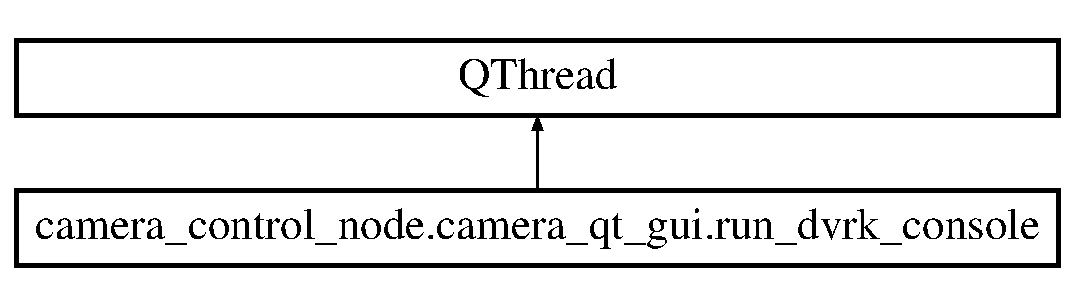
\includegraphics[height=2.000000cm]{classcamera__control__node_1_1camera__qt__gui_1_1run__dvrk__console}
\end{center}
\end{figure}
\subsection*{Public Member Functions}
\begin{DoxyCompactItemize}
\item 
\hypertarget{classcamera__control__node_1_1camera__qt__gui_1_1run__dvrk__console_a950f4ed0605a6e98ddfff327c6051b98}{def {\bfseries run}}\label{classcamera__control__node_1_1camera__qt__gui_1_1run__dvrk__console_a950f4ed0605a6e98ddfff327c6051b98}

\item 
\hypertarget{classcamera__control__node_1_1camera__qt__gui_1_1run__dvrk__console_a384f8f61a8d2a9b8c870223438f48502}{def {\bfseries kill}}\label{classcamera__control__node_1_1camera__qt__gui_1_1run__dvrk__console_a384f8f61a8d2a9b8c870223438f48502}

\end{DoxyCompactItemize}


The documentation for this class was generated from the following file\-:\begin{DoxyCompactItemize}
\item 
camera\-\_\-control\-\_\-node.\-py\end{DoxyCompactItemize}

\hypertarget{classcamera__control__node_1_1Teleop__class}{\section{camera\-\_\-control\-\_\-node.\-Teleop\-\_\-class Class Reference}
\label{classcamera__control__node_1_1Teleop__class}\index{camera\-\_\-control\-\_\-node.\-Teleop\-\_\-class@{camera\-\_\-control\-\_\-node.\-Teleop\-\_\-class}}
}
\subsection*{Classes}
\begin{DoxyCompactItemize}
\item 
class \hyperlink{classcamera__control__node_1_1Teleop__class_1_1MODE}{M\-O\-D\-E}
\end{DoxyCompactItemize}
\subsection*{Public Member Functions}
\begin{DoxyCompactItemize}
\item 
def \hyperlink{classcamera__control__node_1_1Teleop__class_a9c0c5b407b294c85fe58fe045c6c0bbc}{\-\_\-\-\_\-init\-\_\-\-\_\-}
\begin{DoxyCompactList}\small\item\em Initialize the parameters for the \hyperlink{classcamera__control__node_1_1Teleop__class}{Teleop\-\_\-class}. \end{DoxyCompactList}\item 
\hypertarget{classcamera__control__node_1_1Teleop__class_ac76b2e93af302ff7af61f6d646445084}{def \hyperlink{classcamera__control__node_1_1Teleop__class_ac76b2e93af302ff7af61f6d646445084}{rehome}}\label{classcamera__control__node_1_1Teleop__class_ac76b2e93af302ff7af61f6d646445084}

\begin{DoxyCompactList}\small\item\em Home all the arms again. \end{DoxyCompactList}\item 
\hypertarget{classcamera__control__node_1_1Teleop__class_abdfa09c4d553ccf3ddf9dab8ff2a789d}{def \hyperlink{classcamera__control__node_1_1Teleop__class_abdfa09c4d553ccf3ddf9dab8ff2a789d}{home\-\_\-arms}}\label{classcamera__control__node_1_1Teleop__class_abdfa09c4d553ccf3ddf9dab8ff2a789d}

\begin{DoxyCompactList}\small\item\em Move the psms and mtms to a preferred initial position. \end{DoxyCompactList}\item 
\hypertarget{classcamera__control__node_1_1Teleop__class_a4efbf44a090e93896242a8d73bed80c2}{def \hyperlink{classcamera__control__node_1_1Teleop__class_a4efbf44a090e93896242a8d73bed80c2}{shutdown}}\label{classcamera__control__node_1_1Teleop__class_a4efbf44a090e93896242a8d73bed80c2}

\begin{DoxyCompactList}\small\item\em Unregister all the ros publishers and subscribers. \end{DoxyCompactList}\item 
\hypertarget{classcamera__control__node_1_1Teleop__class_a9486ebc1dd621f3ed3aa32120d671b8e}{def \hyperlink{classcamera__control__node_1_1Teleop__class_a9486ebc1dd621f3ed3aa32120d671b8e}{shut\-\_\-down}}\label{classcamera__control__node_1_1Teleop__class_a9486ebc1dd621f3ed3aa32120d671b8e}

\begin{DoxyCompactList}\small\item\em Same as shutdown. \end{DoxyCompactList}\item 
def \hyperlink{classcamera__control__node_1_1Teleop__class_a611b6acc2e845d0269b2194ae1c52457}{set\-\_\-mode}
\begin{DoxyCompactList}\small\item\em Set the operation mode to either simulation or hardware. \end{DoxyCompactList}\item 
\hypertarget{classcamera__control__node_1_1Teleop__class_abbb8d5b8c8dfbc2736fb3e1cb28d54f6}{def {\bfseries spin}}\label{classcamera__control__node_1_1Teleop__class_abbb8d5b8c8dfbc2736fb3e1cb28d54f6}

\item 
\hypertarget{classcamera__control__node_1_1Teleop__class_a4ad0f95701d0951b3f758613f5fdc3c5}{def \hyperlink{classcamera__control__node_1_1Teleop__class_a4ad0f95701d0951b3f758613f5fdc3c5}{pause}}\label{classcamera__control__node_1_1Teleop__class_a4ad0f95701d0951b3f758613f5fdc3c5}

\begin{DoxyCompactList}\small\item\em Pause the teleoperation. \end{DoxyCompactList}\item 
\hypertarget{classcamera__control__node_1_1Teleop__class_a55a643e5dfb067fd86426c9aea1a8ec3}{def \hyperlink{classcamera__control__node_1_1Teleop__class_a55a643e5dfb067fd86426c9aea1a8ec3}{resume}}\label{classcamera__control__node_1_1Teleop__class_a55a643e5dfb067fd86426c9aea1a8ec3}

\begin{DoxyCompactList}\small\item\em Resume the teleopration. \end{DoxyCompactList}\item 
\hypertarget{classcamera__control__node_1_1Teleop__class_a4f6e515dab9822f8513ad23da7be7b36}{def \hyperlink{classcamera__control__node_1_1Teleop__class_a4f6e515dab9822f8513ad23da7be7b36}{enable\-\_\-teleop}}\label{classcamera__control__node_1_1Teleop__class_a4f6e515dab9822f8513ad23da7be7b36}

\begin{DoxyCompactList}\small\item\em Enable teleoperation. \end{DoxyCompactList}\item 
\hypertarget{classcamera__control__node_1_1Teleop__class_a0cd67e1acfe8351955a64b0b64db1e4c}{def \hyperlink{classcamera__control__node_1_1Teleop__class_a0cd67e1acfe8351955a64b0b64db1e4c}{disable\-\_\-teleop}}\label{classcamera__control__node_1_1Teleop__class_a0cd67e1acfe8351955a64b0b64db1e4c}

\begin{DoxyCompactList}\small\item\em Disable teleoperation. \end{DoxyCompactList}\item 
def \hyperlink{classcamera__control__node_1_1Teleop__class_aa78815b8b1658cbcfb27884dbc7a18c9}{rotate}
\begin{DoxyCompactList}\small\item\em Returns a rotation matrix and a transformation matrix. \end{DoxyCompactList}\item 
\hypertarget{classcamera__control__node_1_1Teleop__class_a6ce4ac6cf0fa31b92c3bbb2243f872ea}{def \hyperlink{classcamera__control__node_1_1Teleop__class_a6ce4ac6cf0fa31b92c3bbb2243f872ea}{lock\-\_\-mtm\-\_\-orientations}}\label{classcamera__control__node_1_1Teleop__class_a6ce4ac6cf0fa31b92c3bbb2243f872ea}

\begin{DoxyCompactList}\small\item\em Lock the orientations of M\-T\-Ms. \end{DoxyCompactList}\item 
\hypertarget{classcamera__control__node_1_1Teleop__class_a319d4bc069613f66678c92a0f84335a7}{def \hyperlink{classcamera__control__node_1_1Teleop__class_a319d4bc069613f66678c92a0f84335a7}{\-\_\-\-\_\-clutch\-\_\-cb\-\_\-\-\_\-}}\label{classcamera__control__node_1_1Teleop__class_a319d4bc069613f66678c92a0f84335a7}

\begin{DoxyCompactList}\small\item\em Handle the repositioning clutch. \end{DoxyCompactList}\item 
\hypertarget{classcamera__control__node_1_1Teleop__class_a001d48af70c89abcc97d8f17de43effe}{def \hyperlink{classcamera__control__node_1_1Teleop__class_a001d48af70c89abcc97d8f17de43effe}{\-\_\-\-\_\-headsensor\-\_\-cb\-\_\-\-\_\-}}\label{classcamera__control__node_1_1Teleop__class_a001d48af70c89abcc97d8f17de43effe}

\begin{DoxyCompactList}\small\item\em Callback for the head sensor. \end{DoxyCompactList}\item 
\hypertarget{classcamera__control__node_1_1Teleop__class_ae13fa9f52fcfa6635b9df706ac8056e4}{def \hyperlink{classcamera__control__node_1_1Teleop__class_ae13fa9f52fcfa6635b9df706ac8056e4}{\-\_\-\-\_\-ecm\-\_\-cb\-\_\-\-\_\-}}\label{classcamera__control__node_1_1Teleop__class_ae13fa9f52fcfa6635b9df706ac8056e4}

\begin{DoxyCompactList}\small\item\em Store the E\-C\-M joint angles and end-\/effector position every time a new message is received. \end{DoxyCompactList}\item 
\hypertarget{classcamera__control__node_1_1Teleop__class_a50fb7e9fcae8d34ef9e55f0bfd2fe556}{def \hyperlink{classcamera__control__node_1_1Teleop__class_a50fb7e9fcae8d34ef9e55f0bfd2fe556}{\-\_\-\-\_\-psm1\-\_\-cb\-\_\-\-\_\-}}\label{classcamera__control__node_1_1Teleop__class_a50fb7e9fcae8d34ef9e55f0bfd2fe556}

\begin{DoxyCompactList}\small\item\em Store P\-S\-M joint angles, and move the simulation if the hardware is active. \end{DoxyCompactList}\item 
\hypertarget{classcamera__control__node_1_1Teleop__class_a31ebacabdaedc801b01412c81cf724a4}{def \hyperlink{classcamera__control__node_1_1Teleop__class_a31ebacabdaedc801b01412c81cf724a4}{\-\_\-\-\_\-psm2\-\_\-cb\-\_\-\-\_\-}}\label{classcamera__control__node_1_1Teleop__class_a31ebacabdaedc801b01412c81cf724a4}

\begin{DoxyCompactList}\small\item\em Store P\-S\-M joint angles, and move the simulation if the hardware is active. \end{DoxyCompactList}\item 
\hypertarget{classcamera__control__node_1_1Teleop__class_ae49f0d97f251087fa57405ff80fbd096}{def \hyperlink{classcamera__control__node_1_1Teleop__class_ae49f0d97f251087fa57405ff80fbd096}{\-\_\-\-\_\-mtml\-\_\-gripper\-\_\-cb\-\_\-\-\_\-}}\label{classcamera__control__node_1_1Teleop__class_ae49f0d97f251087fa57405ff80fbd096}

\begin{DoxyCompactList}\small\item\em Record position of the gripper. \end{DoxyCompactList}\item 
\hypertarget{classcamera__control__node_1_1Teleop__class_acede2659e1f07f7f71e08b946ec7534b}{def {\bfseries \-\_\-\-\_\-mtmr\-\_\-gripper\-\_\-cb\-\_\-\-\_\-}}\label{classcamera__control__node_1_1Teleop__class_acede2659e1f07f7f71e08b946ec7534b}

\item 
\hypertarget{classcamera__control__node_1_1Teleop__class_a308840971430d6dfcc4ddf4f7b21211c}{def \hyperlink{classcamera__control__node_1_1Teleop__class_a308840971430d6dfcc4ddf4f7b21211c}{\-\_\-\-\_\-mtml\-\_\-cb\-\_\-\-\_\-}}\label{classcamera__control__node_1_1Teleop__class_a308840971430d6dfcc4ddf4f7b21211c}

\begin{DoxyCompactList}\small\item\em The main part of the teleoperation is performed in this callback function. \end{DoxyCompactList}\item 
\hypertarget{classcamera__control__node_1_1Teleop__class_a5ec0dd8b9519a916fab0134d47b2b582}{def {\bfseries \-\_\-\-\_\-mtmr\-\_\-cb\-\_\-\-\_\-}}\label{classcamera__control__node_1_1Teleop__class_a5ec0dd8b9519a916fab0134d47b2b582}

\item 
\hypertarget{classcamera__control__node_1_1Teleop__class_ab23e1cbbb273a6bb791525a7699a390f}{def {\bfseries \-\_\-\-\_\-translate\-\_\-mtml\-\_\-\-\_\-}}\label{classcamera__control__node_1_1Teleop__class_ab23e1cbbb273a6bb791525a7699a390f}

\item 
\hypertarget{classcamera__control__node_1_1Teleop__class_a05f11974276832eb7bbde4cc2bc64458}{def {\bfseries \-\_\-\-\_\-translate\-\_\-mtmr\-\_\-\-\_\-}}\label{classcamera__control__node_1_1Teleop__class_a05f11974276832eb7bbde4cc2bc64458}

\item 
\hypertarget{classcamera__control__node_1_1Teleop__class_a3c7c891e085be33db256a0781ea485a4}{def {\bfseries \-\_\-\-\_\-set\-\_\-orientation\-\_\-mtml\-\_\-\-\_\-}}\label{classcamera__control__node_1_1Teleop__class_a3c7c891e085be33db256a0781ea485a4}

\item 
\hypertarget{classcamera__control__node_1_1Teleop__class_af391e17fef93c81ddc1fd44f71263d79}{def {\bfseries \-\_\-\-\_\-set\-\_\-orientation\-\_\-mtmr\-\_\-\-\_\-}}\label{classcamera__control__node_1_1Teleop__class_af391e17fef93c81ddc1fd44f71263d79}

\end{DoxyCompactItemize}
\subsection*{Public Attributes}
\begin{DoxyCompactItemize}
\item 
\hypertarget{classcamera__control__node_1_1Teleop__class_abb206f73fc0f76fa869f6e27d62bc728}{\hyperlink{classcamera__control__node_1_1Teleop__class_abb206f73fc0f76fa869f6e27d62bc728}{scale}}\label{classcamera__control__node_1_1Teleop__class_abb206f73fc0f76fa869f6e27d62bc728}

\begin{DoxyCompactList}\small\item\em The scale of movements from M\-T\-Ms to P\-S\-Ms. \end{DoxyCompactList}\end{DoxyCompactItemize}


\subsection{Constructor \& Destructor Documentation}
\hypertarget{classcamera__control__node_1_1Teleop__class_a9c0c5b407b294c85fe58fe045c6c0bbc}{\index{camera\-\_\-control\-\_\-node\-::\-Teleop\-\_\-class@{camera\-\_\-control\-\_\-node\-::\-Teleop\-\_\-class}!\-\_\-\-\_\-init\-\_\-\-\_\-@{\-\_\-\-\_\-init\-\_\-\-\_\-}}
\index{\-\_\-\-\_\-init\-\_\-\-\_\-@{\-\_\-\-\_\-init\-\_\-\-\_\-}!camera_control_node::Teleop_class@{camera\-\_\-control\-\_\-node\-::\-Teleop\-\_\-class}}
\subsubsection[{\-\_\-\-\_\-init\-\_\-\-\_\-}]{\setlength{\rightskip}{0pt plus 5cm}def camera\-\_\-control\-\_\-node.\-Teleop\-\_\-class.\-\_\-\-\_\-init\-\_\-\-\_\- (
\begin{DoxyParamCaption}
\item[{}]{self, }
\item[{}]{mode = {\ttfamily MODE.simulation}}
\end{DoxyParamCaption}
)}}\label{classcamera__control__node_1_1Teleop__class_a9c0c5b407b294c85fe58fe045c6c0bbc}


Initialize the parameters for the \hyperlink{classcamera__control__node_1_1Teleop__class}{Teleop\-\_\-class}. 


\begin{DoxyParams}{Parameters}
{\em mode} & \-: hardwre or simulation mode \\
\hline
\end{DoxyParams}


\subsection{Member Function Documentation}
\hypertarget{classcamera__control__node_1_1Teleop__class_aa78815b8b1658cbcfb27884dbc7a18c9}{\index{camera\-\_\-control\-\_\-node\-::\-Teleop\-\_\-class@{camera\-\_\-control\-\_\-node\-::\-Teleop\-\_\-class}!rotate@{rotate}}
\index{rotate@{rotate}!camera_control_node::Teleop_class@{camera\-\_\-control\-\_\-node\-::\-Teleop\-\_\-class}}
\subsubsection[{rotate}]{\setlength{\rightskip}{0pt plus 5cm}def camera\-\_\-control\-\_\-node.\-Teleop\-\_\-class.\-rotate (
\begin{DoxyParamCaption}
\item[{}]{self, }
\item[{}]{axis, }
\item[{}]{angle}
\end{DoxyParamCaption}
)}}\label{classcamera__control__node_1_1Teleop__class_aa78815b8b1658cbcfb27884dbc7a18c9}


Returns a rotation matrix and a transformation matrix. 


\begin{DoxyParams}{Parameters}
{\em axis} & \-: 'x','y' or 'z' \\
\hline
{\em angle} & \-: In radians \\
\hline
\end{DoxyParams}
\begin{DoxyReturn}{Returns}
r \-: a 3x3 rotation matrix 

t \-: a 4x4 transformation matrix 
\end{DoxyReturn}
\hypertarget{classcamera__control__node_1_1Teleop__class_a611b6acc2e845d0269b2194ae1c52457}{\index{camera\-\_\-control\-\_\-node\-::\-Teleop\-\_\-class@{camera\-\_\-control\-\_\-node\-::\-Teleop\-\_\-class}!set\-\_\-mode@{set\-\_\-mode}}
\index{set\-\_\-mode@{set\-\_\-mode}!camera_control_node::Teleop_class@{camera\-\_\-control\-\_\-node\-::\-Teleop\-\_\-class}}
\subsubsection[{set\-\_\-mode}]{\setlength{\rightskip}{0pt plus 5cm}def camera\-\_\-control\-\_\-node.\-Teleop\-\_\-class.\-set\-\_\-mode (
\begin{DoxyParamCaption}
\item[{}]{self, }
\item[{}]{mode}
\end{DoxyParamCaption}
)}}\label{classcamera__control__node_1_1Teleop__class_a611b6acc2e845d0269b2194ae1c52457}


Set the operation mode to either simulation or hardware. 


\begin{DoxyParams}{Parameters}
{\em mode} & \-: M\-O\-D\-E.\-simulation or M\-O\-D\-E.\-hardware \\
\hline
\end{DoxyParams}


The documentation for this class was generated from the following file\-:\begin{DoxyCompactItemize}
\item 
camera\-\_\-control\-\_\-node.\-py\end{DoxyCompactItemize}

\hypertarget{classcamera__control__node_1_1camera__qt__gui_1_1thread__autocamera}{\section{camera\-\_\-control\-\_\-node.\-camera\-\_\-qt\-\_\-gui.\-thread\-\_\-autocamera Class Reference}
\label{classcamera__control__node_1_1camera__qt__gui_1_1thread__autocamera}\index{camera\-\_\-control\-\_\-node.\-camera\-\_\-qt\-\_\-gui.\-thread\-\_\-autocamera@{camera\-\_\-control\-\_\-node.\-camera\-\_\-qt\-\_\-gui.\-thread\-\_\-autocamera}}
}
Inheritance diagram for camera\-\_\-control\-\_\-node.\-camera\-\_\-qt\-\_\-gui.\-thread\-\_\-autocamera\-:\begin{figure}[H]
\begin{center}
\leavevmode
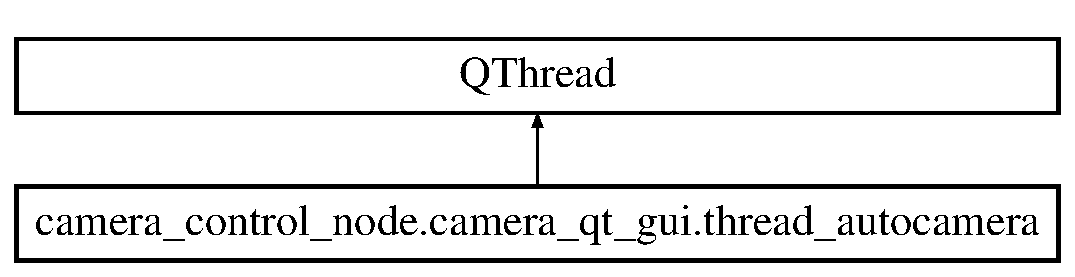
\includegraphics[height=2.000000cm]{classcamera__control__node_1_1camera__qt__gui_1_1thread__autocamera}
\end{center}
\end{figure}
\subsection*{Public Member Functions}
\begin{DoxyCompactItemize}
\item 
\hypertarget{classcamera__control__node_1_1camera__qt__gui_1_1thread__autocamera_af345ff75eaf43936dae83e24247846c7}{def {\bfseries \-\_\-\-\_\-init\-\_\-\-\_\-}}\label{classcamera__control__node_1_1camera__qt__gui_1_1thread__autocamera_af345ff75eaf43936dae83e24247846c7}

\item 
\hypertarget{classcamera__control__node_1_1camera__qt__gui_1_1thread__autocamera_a4be49c185735acde1c4fb7a37cd4c629}{def {\bfseries run}}\label{classcamera__control__node_1_1camera__qt__gui_1_1thread__autocamera_a4be49c185735acde1c4fb7a37cd4c629}

\item 
\hypertarget{classcamera__control__node_1_1camera__qt__gui_1_1thread__autocamera_ac4eb62e38449c8be081de332cc581209}{def {\bfseries kill}}\label{classcamera__control__node_1_1camera__qt__gui_1_1thread__autocamera_ac4eb62e38449c8be081de332cc581209}

\end{DoxyCompactItemize}
\subsection*{Public Attributes}
\begin{DoxyCompactItemize}
\item 
\hypertarget{classcamera__control__node_1_1camera__qt__gui_1_1thread__autocamera_a9216a69b6117ce1bccd2c3cc6ae9eb43}{{\bfseries node\-\_\-handler}}\label{classcamera__control__node_1_1camera__qt__gui_1_1thread__autocamera_a9216a69b6117ce1bccd2c3cc6ae9eb43}

\end{DoxyCompactItemize}


The documentation for this class was generated from the following file\-:\begin{DoxyCompactItemize}
\item 
camera\-\_\-control\-\_\-node.\-py\end{DoxyCompactItemize}

\hypertarget{classcamera__control__node_1_1camera__qt__gui_1_1thread__bag__writer}{\section{camera\-\_\-control\-\_\-node.\-camera\-\_\-qt\-\_\-gui.\-thread\-\_\-bag\-\_\-writer Class Reference}
\label{classcamera__control__node_1_1camera__qt__gui_1_1thread__bag__writer}\index{camera\-\_\-control\-\_\-node.\-camera\-\_\-qt\-\_\-gui.\-thread\-\_\-bag\-\_\-writer@{camera\-\_\-control\-\_\-node.\-camera\-\_\-qt\-\_\-gui.\-thread\-\_\-bag\-\_\-writer}}
}
Inheritance diagram for camera\-\_\-control\-\_\-node.\-camera\-\_\-qt\-\_\-gui.\-thread\-\_\-bag\-\_\-writer\-:\begin{figure}[H]
\begin{center}
\leavevmode
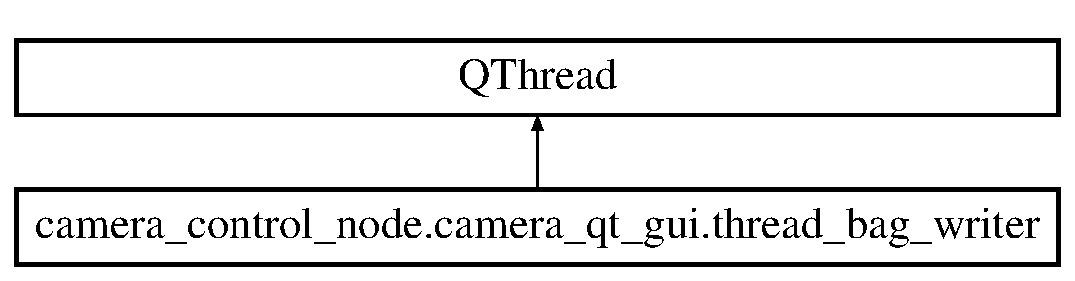
\includegraphics[height=2.000000cm]{classcamera__control__node_1_1camera__qt__gui_1_1thread__bag__writer}
\end{center}
\end{figure}
\subsection*{Public Member Functions}
\begin{DoxyCompactItemize}
\item 
\hypertarget{classcamera__control__node_1_1camera__qt__gui_1_1thread__bag__writer_a7f39f39449e3067a0207da3a9302b2f4}{def {\bfseries \-\_\-\-\_\-init\-\_\-\-\_\-}}\label{classcamera__control__node_1_1camera__qt__gui_1_1thread__bag__writer_a7f39f39449e3067a0207da3a9302b2f4}

\item 
\hypertarget{classcamera__control__node_1_1camera__qt__gui_1_1thread__bag__writer_afdcf20619393441fd713c407db595944}{def {\bfseries run}}\label{classcamera__control__node_1_1camera__qt__gui_1_1thread__bag__writer_afdcf20619393441fd713c407db595944}

\item 
\hypertarget{classcamera__control__node_1_1camera__qt__gui_1_1thread__bag__writer_a420f8844759e32b87ae27908d1291f0c}{def {\bfseries kill}}\label{classcamera__control__node_1_1camera__qt__gui_1_1thread__bag__writer_a420f8844759e32b87ae27908d1291f0c}

\end{DoxyCompactItemize}
\subsection*{Public Attributes}
\begin{DoxyCompactItemize}
\item 
\hypertarget{classcamera__control__node_1_1camera__qt__gui_1_1thread__bag__writer_a1afa2b041166ee4e7de1c328c085dcf9}{{\bfseries node\-\_\-handler}}\label{classcamera__control__node_1_1camera__qt__gui_1_1thread__bag__writer_a1afa2b041166ee4e7de1c328c085dcf9}

\item 
\hypertarget{classcamera__control__node_1_1camera__qt__gui_1_1thread__bag__writer_adee95e934075939075c876e241fc8d3f}{{\bfseries arm\-\_\-names}}\label{classcamera__control__node_1_1camera__qt__gui_1_1thread__bag__writer_adee95e934075939075c876e241fc8d3f}

\item 
\hypertarget{classcamera__control__node_1_1camera__qt__gui_1_1thread__bag__writer_a75eb69ef18c557625997e0aca6ee0fc4}{{\bfseries file\-\_\-name}}\label{classcamera__control__node_1_1camera__qt__gui_1_1thread__bag__writer_a75eb69ef18c557625997e0aca6ee0fc4}

\item 
\hypertarget{classcamera__control__node_1_1camera__qt__gui_1_1thread__bag__writer_ad5ab337027f24baa9b6834558ca1fa7e}{{\bfseries recording\-\_\-dir}}\label{classcamera__control__node_1_1camera__qt__gui_1_1thread__bag__writer_ad5ab337027f24baa9b6834558ca1fa7e}

\end{DoxyCompactItemize}


The documentation for this class was generated from the following file\-:\begin{DoxyCompactItemize}
\item 
camera\-\_\-control\-\_\-node.\-py\end{DoxyCompactItemize}

\hypertarget{classcamera__control__node_1_1camera__qt__gui_1_1thread__clutchNGo}{\section{camera\-\_\-control\-\_\-node.\-camera\-\_\-qt\-\_\-gui.\-thread\-\_\-clutch\-N\-Go Class Reference}
\label{classcamera__control__node_1_1camera__qt__gui_1_1thread__clutchNGo}\index{camera\-\_\-control\-\_\-node.\-camera\-\_\-qt\-\_\-gui.\-thread\-\_\-clutch\-N\-Go@{camera\-\_\-control\-\_\-node.\-camera\-\_\-qt\-\_\-gui.\-thread\-\_\-clutch\-N\-Go}}
}
Inheritance diagram for camera\-\_\-control\-\_\-node.\-camera\-\_\-qt\-\_\-gui.\-thread\-\_\-clutch\-N\-Go\-:\begin{figure}[H]
\begin{center}
\leavevmode
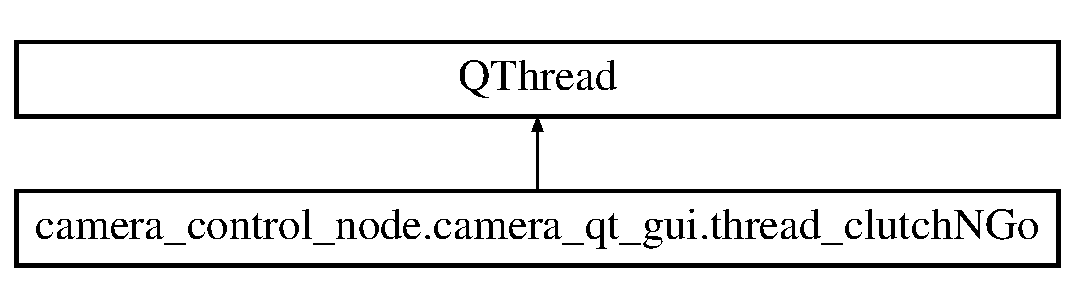
\includegraphics[height=2.000000cm]{classcamera__control__node_1_1camera__qt__gui_1_1thread__clutchNGo}
\end{center}
\end{figure}
\subsection*{Public Member Functions}
\begin{DoxyCompactItemize}
\item 
\hypertarget{classcamera__control__node_1_1camera__qt__gui_1_1thread__clutchNGo_a1a03b0b0d011607d46a2e6576b7f9eca}{def {\bfseries \-\_\-\-\_\-init\-\_\-\-\_\-}}\label{classcamera__control__node_1_1camera__qt__gui_1_1thread__clutchNGo_a1a03b0b0d011607d46a2e6576b7f9eca}

\item 
\hypertarget{classcamera__control__node_1_1camera__qt__gui_1_1thread__clutchNGo_a9de406eefce2f1861abcc956623284bf}{def {\bfseries run}}\label{classcamera__control__node_1_1camera__qt__gui_1_1thread__clutchNGo_a9de406eefce2f1861abcc956623284bf}

\item 
\hypertarget{classcamera__control__node_1_1camera__qt__gui_1_1thread__clutchNGo_a8faf1b8308702796f02ba59ab14373c2}{def {\bfseries kill}}\label{classcamera__control__node_1_1camera__qt__gui_1_1thread__clutchNGo_a8faf1b8308702796f02ba59ab14373c2}

\end{DoxyCompactItemize}
\subsection*{Public Attributes}
\begin{DoxyCompactItemize}
\item 
\hypertarget{classcamera__control__node_1_1camera__qt__gui_1_1thread__clutchNGo_a88f44efe5e4ba7838aa9fee2942f815a}{{\bfseries node\-\_\-handler}}\label{classcamera__control__node_1_1camera__qt__gui_1_1thread__clutchNGo_a88f44efe5e4ba7838aa9fee2942f815a}

\item 
\hypertarget{classcamera__control__node_1_1camera__qt__gui_1_1thread__clutchNGo_a349fe7d8347d58f790291e344556f5ed}{{\bfseries teleop\-\_\-thread}}\label{classcamera__control__node_1_1camera__qt__gui_1_1thread__clutchNGo_a349fe7d8347d58f790291e344556f5ed}

\end{DoxyCompactItemize}


The documentation for this class was generated from the following file\-:\begin{DoxyCompactItemize}
\item 
camera\-\_\-control\-\_\-node.\-py\end{DoxyCompactItemize}

\hypertarget{classcamera__control__node_1_1camera__qt__gui_1_1thread__home__arms}{\section{camera\-\_\-control\-\_\-node.\-camera\-\_\-qt\-\_\-gui.\-thread\-\_\-home\-\_\-arms Class Reference}
\label{classcamera__control__node_1_1camera__qt__gui_1_1thread__home__arms}\index{camera\-\_\-control\-\_\-node.\-camera\-\_\-qt\-\_\-gui.\-thread\-\_\-home\-\_\-arms@{camera\-\_\-control\-\_\-node.\-camera\-\_\-qt\-\_\-gui.\-thread\-\_\-home\-\_\-arms}}
}
Inheritance diagram for camera\-\_\-control\-\_\-node.\-camera\-\_\-qt\-\_\-gui.\-thread\-\_\-home\-\_\-arms\-:\begin{figure}[H]
\begin{center}
\leavevmode
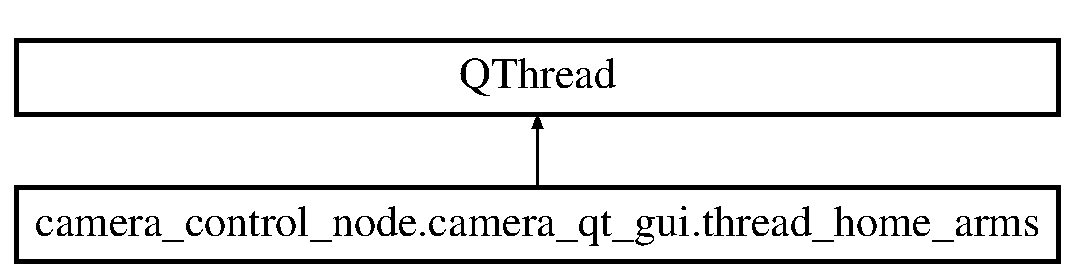
\includegraphics[height=2.000000cm]{classcamera__control__node_1_1camera__qt__gui_1_1thread__home__arms}
\end{center}
\end{figure}
\subsection*{Public Member Functions}
\begin{DoxyCompactItemize}
\item 
\hypertarget{classcamera__control__node_1_1camera__qt__gui_1_1thread__home__arms_a120fc8a711b3b49b8af9fac00c975b0a}{def {\bfseries \-\_\-\-\_\-init\-\_\-\-\_\-}}\label{classcamera__control__node_1_1camera__qt__gui_1_1thread__home__arms_a120fc8a711b3b49b8af9fac00c975b0a}

\item 
\hypertarget{classcamera__control__node_1_1camera__qt__gui_1_1thread__home__arms_af7ddce6b31eb38db57f1d9156d6527b1}{def {\bfseries run}}\label{classcamera__control__node_1_1camera__qt__gui_1_1thread__home__arms_af7ddce6b31eb38db57f1d9156d6527b1}

\item 
\hypertarget{classcamera__control__node_1_1camera__qt__gui_1_1thread__home__arms_abc53a2d4089b0cc6aa21b72c1f66942a}{def {\bfseries home}}\label{classcamera__control__node_1_1camera__qt__gui_1_1thread__home__arms_abc53a2d4089b0cc6aa21b72c1f66942a}

\item 
\hypertarget{classcamera__control__node_1_1camera__qt__gui_1_1thread__home__arms_a182fa869199ea677a5c6a9849ebcbb3a}{def {\bfseries kill}}\label{classcamera__control__node_1_1camera__qt__gui_1_1thread__home__arms_a182fa869199ea677a5c6a9849ebcbb3a}

\end{DoxyCompactItemize}
\subsection*{Public Attributes}
\begin{DoxyCompactItemize}
\item 
\hypertarget{classcamera__control__node_1_1camera__qt__gui_1_1thread__home__arms_a389c4c7ae670151b39e08fa53fc934ab}{{\bfseries is\-\_\-running}}\label{classcamera__control__node_1_1camera__qt__gui_1_1thread__home__arms_a389c4c7ae670151b39e08fa53fc934ab}

\item 
\hypertarget{classcamera__control__node_1_1camera__qt__gui_1_1thread__home__arms_a1ff7c77b70e5ac413ca9b80502d3ea95}{{\bfseries ecm}}\label{classcamera__control__node_1_1camera__qt__gui_1_1thread__home__arms_a1ff7c77b70e5ac413ca9b80502d3ea95}

\end{DoxyCompactItemize}


The documentation for this class was generated from the following file\-:\begin{DoxyCompactItemize}
\item 
camera\-\_\-control\-\_\-node.\-py\end{DoxyCompactItemize}

\hypertarget{classcamera__control__node_1_1camera__qt__gui_1_1thread__joystick}{\section{camera\-\_\-control\-\_\-node.\-camera\-\_\-qt\-\_\-gui.\-thread\-\_\-joystick Class Reference}
\label{classcamera__control__node_1_1camera__qt__gui_1_1thread__joystick}\index{camera\-\_\-control\-\_\-node.\-camera\-\_\-qt\-\_\-gui.\-thread\-\_\-joystick@{camera\-\_\-control\-\_\-node.\-camera\-\_\-qt\-\_\-gui.\-thread\-\_\-joystick}}
}
Inheritance diagram for camera\-\_\-control\-\_\-node.\-camera\-\_\-qt\-\_\-gui.\-thread\-\_\-joystick\-:\begin{figure}[H]
\begin{center}
\leavevmode
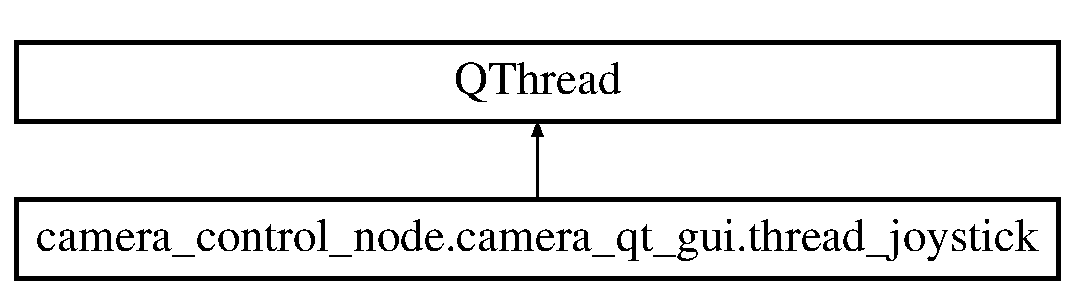
\includegraphics[height=2.000000cm]{classcamera__control__node_1_1camera__qt__gui_1_1thread__joystick}
\end{center}
\end{figure}
\subsection*{Public Member Functions}
\begin{DoxyCompactItemize}
\item 
\hypertarget{classcamera__control__node_1_1camera__qt__gui_1_1thread__joystick_a2834483cb6e2a15b9954b670d58f69ef}{def {\bfseries \-\_\-\-\_\-init\-\_\-\-\_\-}}\label{classcamera__control__node_1_1camera__qt__gui_1_1thread__joystick_a2834483cb6e2a15b9954b670d58f69ef}

\item 
\hypertarget{classcamera__control__node_1_1camera__qt__gui_1_1thread__joystick_ab746b4a7047a850cfd5c9e3c321d2c38}{def {\bfseries run}}\label{classcamera__control__node_1_1camera__qt__gui_1_1thread__joystick_ab746b4a7047a850cfd5c9e3c321d2c38}

\item 
\hypertarget{classcamera__control__node_1_1camera__qt__gui_1_1thread__joystick_ac0f60b163bab3c3d3c80c304b3bc679b}{def {\bfseries kill}}\label{classcamera__control__node_1_1camera__qt__gui_1_1thread__joystick_ac0f60b163bab3c3d3c80c304b3bc679b}

\end{DoxyCompactItemize}
\subsection*{Public Attributes}
\begin{DoxyCompactItemize}
\item 
\hypertarget{classcamera__control__node_1_1camera__qt__gui_1_1thread__joystick_a12dc8897aa5f07e6e6e6c0e1ab857e6b}{{\bfseries node\-\_\-handler}}\label{classcamera__control__node_1_1camera__qt__gui_1_1thread__joystick_a12dc8897aa5f07e6e6e6c0e1ab857e6b}

\end{DoxyCompactItemize}


The documentation for this class was generated from the following file\-:\begin{DoxyCompactItemize}
\item 
camera\-\_\-control\-\_\-node.\-py\end{DoxyCompactItemize}

\hypertarget{classcamera__control__node_1_1camera__qt__gui_1_1thread__oculus}{\section{camera\-\_\-control\-\_\-node.\-camera\-\_\-qt\-\_\-gui.\-thread\-\_\-oculus Class Reference}
\label{classcamera__control__node_1_1camera__qt__gui_1_1thread__oculus}\index{camera\-\_\-control\-\_\-node.\-camera\-\_\-qt\-\_\-gui.\-thread\-\_\-oculus@{camera\-\_\-control\-\_\-node.\-camera\-\_\-qt\-\_\-gui.\-thread\-\_\-oculus}}
}
Inheritance diagram for camera\-\_\-control\-\_\-node.\-camera\-\_\-qt\-\_\-gui.\-thread\-\_\-oculus\-:\begin{figure}[H]
\begin{center}
\leavevmode
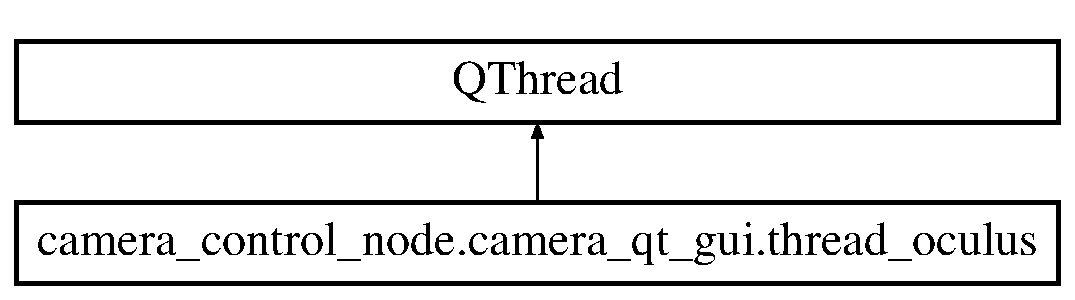
\includegraphics[height=2.000000cm]{classcamera__control__node_1_1camera__qt__gui_1_1thread__oculus}
\end{center}
\end{figure}
\subsection*{Public Member Functions}
\begin{DoxyCompactItemize}
\item 
\hypertarget{classcamera__control__node_1_1camera__qt__gui_1_1thread__oculus_a7d9f273fd95b03cf27040d46b38e8b07}{def {\bfseries \-\_\-\-\_\-init\-\_\-\-\_\-}}\label{classcamera__control__node_1_1camera__qt__gui_1_1thread__oculus_a7d9f273fd95b03cf27040d46b38e8b07}

\item 
\hypertarget{classcamera__control__node_1_1camera__qt__gui_1_1thread__oculus_a10a4701163d581d41976cb42b8661e50}{def {\bfseries run}}\label{classcamera__control__node_1_1camera__qt__gui_1_1thread__oculus_a10a4701163d581d41976cb42b8661e50}

\item 
\hypertarget{classcamera__control__node_1_1camera__qt__gui_1_1thread__oculus_a0c0bcd2e785caf1113d81b31d39344da}{def {\bfseries kill}}\label{classcamera__control__node_1_1camera__qt__gui_1_1thread__oculus_a0c0bcd2e785caf1113d81b31d39344da}

\end{DoxyCompactItemize}
\subsection*{Public Attributes}
\begin{DoxyCompactItemize}
\item 
\hypertarget{classcamera__control__node_1_1camera__qt__gui_1_1thread__oculus_aecc2e1ef045069903ea44b3a0b4776df}{{\bfseries node\-\_\-handler}}\label{classcamera__control__node_1_1camera__qt__gui_1_1thread__oculus_aecc2e1ef045069903ea44b3a0b4776df}

\end{DoxyCompactItemize}


The documentation for this class was generated from the following file\-:\begin{DoxyCompactItemize}
\item 
camera\-\_\-control\-\_\-node.\-py\end{DoxyCompactItemize}

\hypertarget{classcamera__control__node_1_1camera__qt__gui_1_1thread__teleop}{\section{camera\-\_\-control\-\_\-node.\-camera\-\_\-qt\-\_\-gui.\-thread\-\_\-teleop Class Reference}
\label{classcamera__control__node_1_1camera__qt__gui_1_1thread__teleop}\index{camera\-\_\-control\-\_\-node.\-camera\-\_\-qt\-\_\-gui.\-thread\-\_\-teleop@{camera\-\_\-control\-\_\-node.\-camera\-\_\-qt\-\_\-gui.\-thread\-\_\-teleop}}
}
Inheritance diagram for camera\-\_\-control\-\_\-node.\-camera\-\_\-qt\-\_\-gui.\-thread\-\_\-teleop\-:\begin{figure}[H]
\begin{center}
\leavevmode
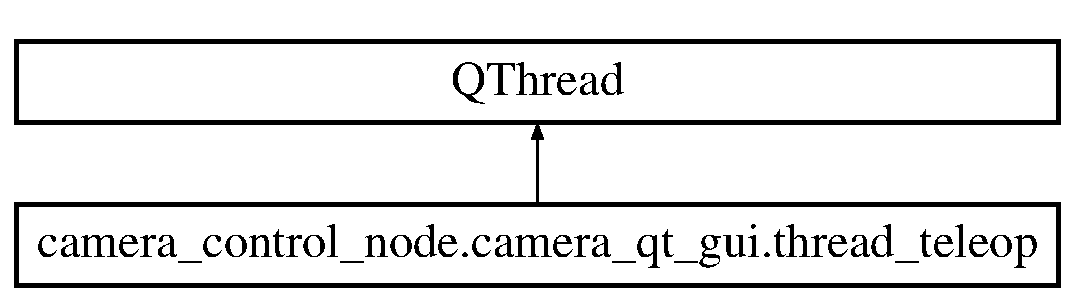
\includegraphics[height=2.000000cm]{classcamera__control__node_1_1camera__qt__gui_1_1thread__teleop}
\end{center}
\end{figure}
\subsection*{Public Member Functions}
\begin{DoxyCompactItemize}
\item 
\hypertarget{classcamera__control__node_1_1camera__qt__gui_1_1thread__teleop_a20dc0ca0d3fc4cff21bb591aade47659}{def {\bfseries \-\_\-\-\_\-init\-\_\-\-\_\-}}\label{classcamera__control__node_1_1camera__qt__gui_1_1thread__teleop_a20dc0ca0d3fc4cff21bb591aade47659}

\item 
\hypertarget{classcamera__control__node_1_1camera__qt__gui_1_1thread__teleop_a6459d69c86fd97058fd4904fd36a7cce}{def {\bfseries run}}\label{classcamera__control__node_1_1camera__qt__gui_1_1thread__teleop_a6459d69c86fd97058fd4904fd36a7cce}

\item 
\hypertarget{classcamera__control__node_1_1camera__qt__gui_1_1thread__teleop_a1791c04cd025c9d2d1cdc7ad2567f114}{def {\bfseries kill}}\label{classcamera__control__node_1_1camera__qt__gui_1_1thread__teleop_a1791c04cd025c9d2d1cdc7ad2567f114}

\item 
\hypertarget{classcamera__control__node_1_1camera__qt__gui_1_1thread__teleop_a1006c3ffdbacf0b26fa7ae799148e714}{def {\bfseries home}}\label{classcamera__control__node_1_1camera__qt__gui_1_1thread__teleop_a1006c3ffdbacf0b26fa7ae799148e714}

\item 
\hypertarget{classcamera__control__node_1_1camera__qt__gui_1_1thread__teleop_a8ebda1ce64984ed4657c21bf091c34e0}{def {\bfseries pause}}\label{classcamera__control__node_1_1camera__qt__gui_1_1thread__teleop_a8ebda1ce64984ed4657c21bf091c34e0}

\item 
\hypertarget{classcamera__control__node_1_1camera__qt__gui_1_1thread__teleop_ab9eb5b22d79579dea6b75015f72e5bd0}{def {\bfseries resume}}\label{classcamera__control__node_1_1camera__qt__gui_1_1thread__teleop_ab9eb5b22d79579dea6b75015f72e5bd0}

\item 
\hypertarget{classcamera__control__node_1_1camera__qt__gui_1_1thread__teleop_af83173158b9d7642cea1df41a78d28d4}{def {\bfseries lock\-\_\-mtm\-\_\-orientations}}\label{classcamera__control__node_1_1camera__qt__gui_1_1thread__teleop_af83173158b9d7642cea1df41a78d28d4}

\end{DoxyCompactItemize}
\subsection*{Public Attributes}
\begin{DoxyCompactItemize}
\item 
\hypertarget{classcamera__control__node_1_1camera__qt__gui_1_1thread__teleop_aa5d4d5269d54f4e72d5344eb013c3805}{{\bfseries node\-\_\-handler}}\label{classcamera__control__node_1_1camera__qt__gui_1_1thread__teleop_aa5d4d5269d54f4e72d5344eb013c3805}

\end{DoxyCompactItemize}


The documentation for this class was generated from the following file\-:\begin{DoxyCompactItemize}
\item 
camera\-\_\-control\-\_\-node.\-py\end{DoxyCompactItemize}

\hypertarget{classcamera__control__node_1_1camera__qt__gui_1_1thread__timer}{\section{camera\-\_\-control\-\_\-node.\-camera\-\_\-qt\-\_\-gui.\-thread\-\_\-timer Class Reference}
\label{classcamera__control__node_1_1camera__qt__gui_1_1thread__timer}\index{camera\-\_\-control\-\_\-node.\-camera\-\_\-qt\-\_\-gui.\-thread\-\_\-timer@{camera\-\_\-control\-\_\-node.\-camera\-\_\-qt\-\_\-gui.\-thread\-\_\-timer}}
}
Inheritance diagram for camera\-\_\-control\-\_\-node.\-camera\-\_\-qt\-\_\-gui.\-thread\-\_\-timer\-:\begin{figure}[H]
\begin{center}
\leavevmode
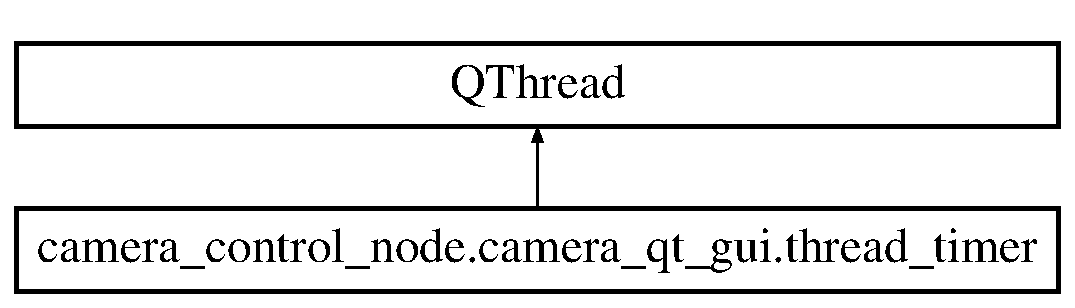
\includegraphics[height=2.000000cm]{classcamera__control__node_1_1camera__qt__gui_1_1thread__timer}
\end{center}
\end{figure}
\subsection*{Public Member Functions}
\begin{DoxyCompactItemize}
\item 
\hypertarget{classcamera__control__node_1_1camera__qt__gui_1_1thread__timer_ab0b7ba23d48e2ecf4573c10230b8d365}{def {\bfseries \-\_\-\-\_\-init\-\_\-\-\_\-}}\label{classcamera__control__node_1_1camera__qt__gui_1_1thread__timer_ab0b7ba23d48e2ecf4573c10230b8d365}

\item 
\hypertarget{classcamera__control__node_1_1camera__qt__gui_1_1thread__timer_a9c92d15e574110bdb76ae78195a5c752}{def {\bfseries setup}}\label{classcamera__control__node_1_1camera__qt__gui_1_1thread__timer_a9c92d15e574110bdb76ae78195a5c752}

\item 
\hypertarget{classcamera__control__node_1_1camera__qt__gui_1_1thread__timer_ab6b55f19686e1f1396818bffabf8b411}{def {\bfseries run}}\label{classcamera__control__node_1_1camera__qt__gui_1_1thread__timer_ab6b55f19686e1f1396818bffabf8b411}

\item 
\hypertarget{classcamera__control__node_1_1camera__qt__gui_1_1thread__timer_ae2e902561cf8cb59bb35f4adfecd2e4e}{def {\bfseries kill}}\label{classcamera__control__node_1_1camera__qt__gui_1_1thread__timer_ae2e902561cf8cb59bb35f4adfecd2e4e}

\end{DoxyCompactItemize}
\subsection*{Public Attributes}
\begin{DoxyCompactItemize}
\item 
\hypertarget{classcamera__control__node_1_1camera__qt__gui_1_1thread__timer_abcb046fcea265aff6535f08f15296066}{{\bfseries thread\-\_\-no}}\label{classcamera__control__node_1_1camera__qt__gui_1_1thread__timer_abcb046fcea265aff6535f08f15296066}

\end{DoxyCompactItemize}
\subsection*{Static Public Attributes}
\begin{DoxyCompactItemize}
\item 
\hypertarget{classcamera__control__node_1_1camera__qt__gui_1_1thread__timer_a16c447fa8f03c6b388f06a723f0e4159}{tuple {\bfseries trigger} = pyqt\-Signal(int)}\label{classcamera__control__node_1_1camera__qt__gui_1_1thread__timer_a16c447fa8f03c6b388f06a723f0e4159}

\end{DoxyCompactItemize}


The documentation for this class was generated from the following file\-:\begin{DoxyCompactItemize}
\item 
camera\-\_\-control\-\_\-node.\-py\end{DoxyCompactItemize}

\hypertarget{classcamera__control__gui_1_1Ui__Dialog}{\section{camera\-\_\-control\-\_\-gui.\-Ui\-\_\-\-Dialog Class Reference}
\label{classcamera__control__gui_1_1Ui__Dialog}\index{camera\-\_\-control\-\_\-gui.\-Ui\-\_\-\-Dialog@{camera\-\_\-control\-\_\-gui.\-Ui\-\_\-\-Dialog}}
}
Inheritance diagram for camera\-\_\-control\-\_\-gui.\-Ui\-\_\-\-Dialog\-:\begin{figure}[H]
\begin{center}
\leavevmode
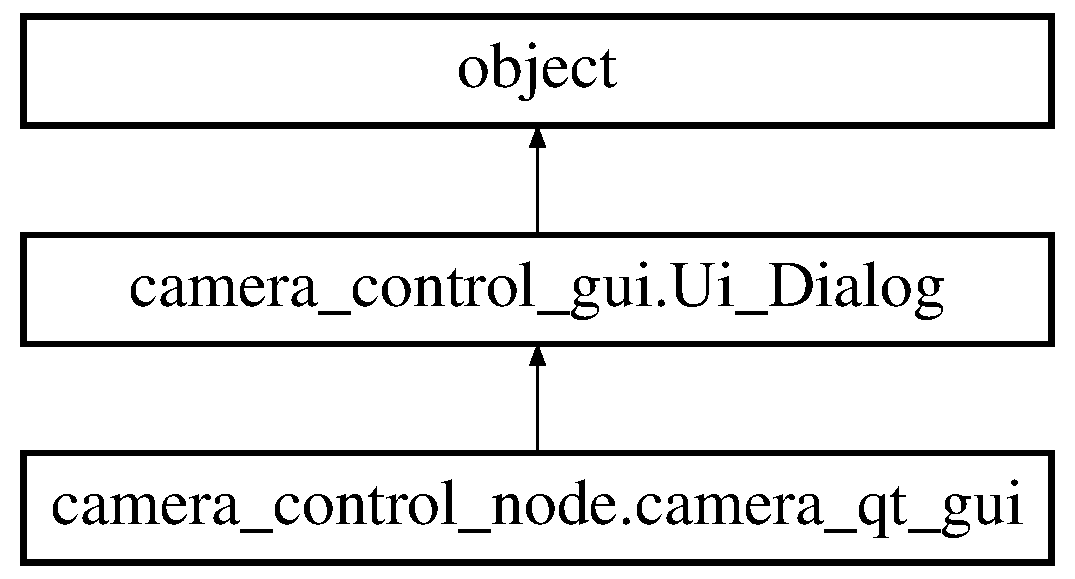
\includegraphics[height=3.000000cm]{classcamera__control__gui_1_1Ui__Dialog}
\end{center}
\end{figure}
\subsection*{Public Member Functions}
\begin{DoxyCompactItemize}
\item 
\hypertarget{classcamera__control__gui_1_1Ui__Dialog_a636de533420a3fed567c7842a5ff2a60}{def {\bfseries setup\-Ui}}\label{classcamera__control__gui_1_1Ui__Dialog_a636de533420a3fed567c7842a5ff2a60}

\item 
\hypertarget{classcamera__control__gui_1_1Ui__Dialog_a9fa49ed45b992f6c267793dc7859f7c9}{def {\bfseries retranslate\-Ui}}\label{classcamera__control__gui_1_1Ui__Dialog_a9fa49ed45b992f6c267793dc7859f7c9}

\end{DoxyCompactItemize}
\subsection*{Public Attributes}
\begin{DoxyCompactItemize}
\item 
\hypertarget{classcamera__control__gui_1_1Ui__Dialog_a41ed9952fea0e5ae708e541668fd6ffa}{{\bfseries group\-Box\-Operation\-Mode}}\label{classcamera__control__gui_1_1Ui__Dialog_a41ed9952fea0e5ae708e541668fd6ffa}

\item 
\hypertarget{classcamera__control__gui_1_1Ui__Dialog_ae3478ef269cbe1e8cbc040907d2d852e}{{\bfseries radio\-Button\-Simulation}}\label{classcamera__control__gui_1_1Ui__Dialog_ae3478ef269cbe1e8cbc040907d2d852e}

\item 
\hypertarget{classcamera__control__gui_1_1Ui__Dialog_a7528849634a651ff21776fa52f352ec2}{{\bfseries radio\-Button\-Hardware}}\label{classcamera__control__gui_1_1Ui__Dialog_a7528849634a651ff21776fa52f352ec2}

\item 
\hypertarget{classcamera__control__gui_1_1Ui__Dialog_a73d5a3134bb1e7978379780295aaed9e}{{\bfseries group\-Box\-Camera\-Control\-Method}}\label{classcamera__control__gui_1_1Ui__Dialog_a73d5a3134bb1e7978379780295aaed9e}

\item 
\hypertarget{classcamera__control__gui_1_1Ui__Dialog_a16a51d265d12d1d8f886578d5cfa2526}{{\bfseries radio\-Button\-Autocamera}}\label{classcamera__control__gui_1_1Ui__Dialog_a16a51d265d12d1d8f886578d5cfa2526}

\item 
\hypertarget{classcamera__control__gui_1_1Ui__Dialog_a9926a4a2aaa9e747956f3f1ea0c5e651}{{\bfseries radio\-Button\-Clutch\-And\-Move}}\label{classcamera__control__gui_1_1Ui__Dialog_a9926a4a2aaa9e747956f3f1ea0c5e651}

\item 
\hypertarget{classcamera__control__gui_1_1Ui__Dialog_a7244013abda0dc2b80dc3ac0f9df0551}{{\bfseries radio\-Button\-Joystick}}\label{classcamera__control__gui_1_1Ui__Dialog_a7244013abda0dc2b80dc3ac0f9df0551}

\item 
\hypertarget{classcamera__control__gui_1_1Ui__Dialog_a1a01120b0584983e8965a5d39fc6161f}{{\bfseries radio\-Button\-Teleop}}\label{classcamera__control__gui_1_1Ui__Dialog_a1a01120b0584983e8965a5d39fc6161f}

\item 
\hypertarget{classcamera__control__gui_1_1Ui__Dialog_afd142a5b9b75fce02b152bc149e863ef}{{\bfseries radio\-Button\-Oculus}}\label{classcamera__control__gui_1_1Ui__Dialog_afd142a5b9b75fce02b152bc149e863ef}

\item 
\hypertarget{classcamera__control__gui_1_1Ui__Dialog_a7659c6b8989a4d15806cc808b1a3dc16}{{\bfseries group\-Box\-Power}}\label{classcamera__control__gui_1_1Ui__Dialog_a7659c6b8989a4d15806cc808b1a3dc16}

\item 
\hypertarget{classcamera__control__gui_1_1Ui__Dialog_a2c2d348b9f1ff009af1df7b149442491}{{\bfseries push\-Button\-Home}}\label{classcamera__control__gui_1_1Ui__Dialog_a2c2d348b9f1ff009af1df7b149442491}

\item 
\hypertarget{classcamera__control__gui_1_1Ui__Dialog_ac9ffba2047ea7853f8a0e54af3680661}{{\bfseries push\-Button\-Power\-Off}}\label{classcamera__control__gui_1_1Ui__Dialog_ac9ffba2047ea7853f8a0e54af3680661}

\item 
\hypertarget{classcamera__control__gui_1_1Ui__Dialog_ac292a75614cbba9bb9954a1091bba012}{{\bfseries push\-Button\-Exit}}\label{classcamera__control__gui_1_1Ui__Dialog_ac292a75614cbba9bb9954a1091bba012}

\item 
\hypertarget{classcamera__control__gui_1_1Ui__Dialog_ac4c3af02faa2d8c324dec79c82f05ec0}{{\bfseries push\-Button\-Power\-On}}\label{classcamera__control__gui_1_1Ui__Dialog_ac4c3af02faa2d8c324dec79c82f05ec0}

\item 
\hypertarget{classcamera__control__gui_1_1Ui__Dialog_a2346eaf80990a45a7ff42ae82d2782fa}{{\bfseries push\-Button\-Reset}}\label{classcamera__control__gui_1_1Ui__Dialog_a2346eaf80990a45a7ff42ae82d2782fa}

\item 
\hypertarget{classcamera__control__gui_1_1Ui__Dialog_a4e973edcaad73653eebc1e3c4d135904}{{\bfseries group\-Box\-Autocamera\-Params}}\label{classcamera__control__gui_1_1Ui__Dialog_a4e973edcaad73653eebc1e3c4d135904}

\item 
\hypertarget{classcamera__control__gui_1_1Ui__Dialog_a08d27060b8464bd976ad5bff53866626}{{\bfseries horizontal\-Slider\-Innerzone}}\label{classcamera__control__gui_1_1Ui__Dialog_a08d27060b8464bd976ad5bff53866626}

\item 
\hypertarget{classcamera__control__gui_1_1Ui__Dialog_a47c42179c6b009804df4b8caed549f4d}{{\bfseries horizontal\-Slider\-Deadzone}}\label{classcamera__control__gui_1_1Ui__Dialog_a47c42179c6b009804df4b8caed549f4d}

\item 
\hypertarget{classcamera__control__gui_1_1Ui__Dialog_aaa6feeb9bc61ed124384065e24475c51}{{\bfseries label\-Innerzone\-Value}}\label{classcamera__control__gui_1_1Ui__Dialog_aaa6feeb9bc61ed124384065e24475c51}

\item 
\hypertarget{classcamera__control__gui_1_1Ui__Dialog_a1759de5ed3f2434614f27c175cc97aec}{{\bfseries label\-Deadzone\-Value}}\label{classcamera__control__gui_1_1Ui__Dialog_a1759de5ed3f2434614f27c175cc97aec}

\item 
\hypertarget{classcamera__control__gui_1_1Ui__Dialog_a4eb4c18ecb4ac9abfbed535efaf21ab4}{{\bfseries label\-\_\-3}}\label{classcamera__control__gui_1_1Ui__Dialog_a4eb4c18ecb4ac9abfbed535efaf21ab4}

\item 
\hypertarget{classcamera__control__gui_1_1Ui__Dialog_a9d8768170d0944c2976e37264d202619}{{\bfseries label\-\_\-4}}\label{classcamera__control__gui_1_1Ui__Dialog_a9d8768170d0944c2976e37264d202619}

\item 
\hypertarget{classcamera__control__gui_1_1Ui__Dialog_acee698c21b24fef66e0b54c0be93152a}{{\bfseries push\-Button\-Record}}\label{classcamera__control__gui_1_1Ui__Dialog_acee698c21b24fef66e0b54c0be93152a}

\item 
\hypertarget{classcamera__control__gui_1_1Ui__Dialog_ad750505345f6ac02fa7273a0713c1512}{{\bfseries label\-Subject\-Info}}\label{classcamera__control__gui_1_1Ui__Dialog_ad750505345f6ac02fa7273a0713c1512}

\item 
\hypertarget{classcamera__control__gui_1_1Ui__Dialog_a14f800d2b3cfd3cb2cd60452cc77eb4b}{{\bfseries label\-Subject\-Number}}\label{classcamera__control__gui_1_1Ui__Dialog_a14f800d2b3cfd3cb2cd60452cc77eb4b}

\item 
\hypertarget{classcamera__control__gui_1_1Ui__Dialog_a6342519b511f8d4ab381d14017aca6f0}{{\bfseries spin\-Box\-Subject\-Number}}\label{classcamera__control__gui_1_1Ui__Dialog_a6342519b511f8d4ab381d14017aca6f0}

\item 
\hypertarget{classcamera__control__gui_1_1Ui__Dialog_a9f23f27389782761db8028c6b991e6fe}{{\bfseries label\-Pattern\-Number}}\label{classcamera__control__gui_1_1Ui__Dialog_a9f23f27389782761db8028c6b991e6fe}

\item 
\hypertarget{classcamera__control__gui_1_1Ui__Dialog_a1e1a777fdf0d94d1e15e9945bf85473e}{{\bfseries spin\-Box\-Pattern\-Number}}\label{classcamera__control__gui_1_1Ui__Dialog_a1e1a777fdf0d94d1e15e9945bf85473e}

\item 
\hypertarget{classcamera__control__gui_1_1Ui__Dialog_a393a561527348e796b3c57402fa8fb51}{{\bfseries label\-Timer}}\label{classcamera__control__gui_1_1Ui__Dialog_a393a561527348e796b3c57402fa8fb51}

\end{DoxyCompactItemize}


The documentation for this class was generated from the following file\-:\begin{DoxyCompactItemize}
\item 
camera\-\_\-control\-\_\-gui.\-py\end{DoxyCompactItemize}

%--- End generated contents ---

% Index
\newpage
\phantomsection
\addcontentsline{toc}{chapter}{Index}
\printindex

\end{document}
